\documentclass[oneside,final]{hcmut-report}

\usepackage{gensymb,textcomp}
\usepackage[table]{xcolor}
\usepackage{array,longtable,multirow,tabularx}
\usepackage{enumitem}
\usepackage{caption,subcaption,float}
\usepackage{xurl}
\usepackage[nameinlink]{cleveref}

\captionsetup{font=small,labelfont=bf,skip=5pt}
\captionsetup[subfigure]{font=footnotesize,skip=3pt}
\setlength{\emergencystretch}{3em}
\setlength{\intextsep}{8pt plus 2pt minus 2pt}
\setlength{\textfloatsep}{10pt plus 2pt minus 2pt}
\setlength{\LTpre}{4pt}
\setlength{\LTpost}{4pt}
\hbadness=10000
\vbadness=10000

\definecolor{tblHeader}{HTML}{EFEFEF}

% Compact list spacing
\setlist[itemize]{topsep=3pt,itemsep=2pt,parsep=0pt,leftmargin=1.4em}
\setlist[enumerate]{topsep=3pt,itemsep=2pt,parsep=0pt,leftmargin=1.5em}

% Full-grid bordered table column types
\newcolumntype{L}[1]{>{\raggedright\arraybackslash}p{#1}}
\newcolumntype{C}[1]{>{\centering\arraybackslash}p{#1}}
\newcolumntype{Y}{>{\raggedright\arraybackslash}X}

% Automatic page-break guard so headings never sit orphaned at page bottom
\newcommand{\safesubsection}[1]{%
  \par\ifdim\pagetotal>0.80\textheight\newpage\fi\subsection{#1}%
}
\newcommand{\safesubsubsection}[1]{%
  \par\ifdim\pagetotal>0.83\textheight\newpage\fi\subsubsection{#1}%
}

% Cover page metadata (Semester 261)
\coursename{SOFTWARE ENGINEERING (CO3001) --- SEMESTER 261}
\reporttype{FINAL PROJECT REPORT --- GROUP 7}
\title{Smart E-Mobility Hub:\\[0.24cm]{\fontsize{13.5pt}{18.5pt}\selectfont Electric Mobility Coordination System for the\\VNU-HCM Urban Area}}
\advisor{Dr.\ Nguyễn Thành Công}
\stuname{%
  & Mã Trần Minh Quốc & (ID: 2353026) \\
  & Lục Khánh Phát & (ID: 2452942) \\
  & Trần Tiến Phát & (ID: 2452950) \\
  & Lê Minh Nhật & (ID: 2452891) \\
  & Phạm Tuấn Minh & (ID: 2452766) \\
  & Nguyễn Thùy Trang & (ID: 2453272) \\
  & Nils Tanguy BOUSQUET & (ID: 2660011) \\
}
\reportplace{Ho Chi Minh City}
\reporttime{November 2026}

\begin{document}
\coverpage

% ============================================================================
% CONCISE TASK ASSIGNMENT TABLE (BORDERED GRID, KEYWORDS ONLY)
% ============================================================================
\section*{Group 7 --- Member List \& Task Assignment}
\addcontentsline{toc}{section}{Group 7 --- Member List \& Task Assignment}

{\singlespacing\small
\renewcommand{\arraystretch}{1.35}
\noindent
\begin{tabularx}{\textwidth}{|C{0.9cm}|L{4.1cm}|C{2.1cm}|Y|C{2.1cm}|}
  \hline
  \rowcolor{tblHeader}
  \textbf{No.} & \textbf{Full Name} & \textbf{Student ID} & \textbf{Assigned Keywords} & \textbf{Workload} \\
  \hline
  1 & Mã Trần Minh Quốc & 2353026 & Frontend Lead, Operator UI, Campus Map, Report & 100\% \\
  \hline
  2 & Lục Khánh Phát & 2452942 & Reservation \& Charging APIs, Class Diagram, ERD, Report & 100\% \\
  \hline
  3 & Trần Tiến Phát & 2452950 & Activity \& State Diagrams, Operator APIs, Mobile QA & 100\% \\
  \hline
  4 & Lê Minh Nhật & 2452891 & System Architecture, Business Rules, Test Plan \& QA & 100\% \\
  \hline
  5 & Phạm Tuấn Minh & 2452766 & Functional Requirements, OpenAPI, Auth \& Integration & 100\% \\
  \hline
  6 & Nguyễn Thùy Trang & 2453272 & Non-Functional Requirements, UI Wireframes, Slide Deck & 100\% \\
  \hline
  7 & Nils Tanguy BOUSQUET & 2660011 & Use-Case \& Sequence Diagrams, What-If Engine, Demo & 100\% \\
  \hline
\end{tabularx}
}

\vspace{10pt}
\noindent\textbf{Source Code Repository:} \url{https://github.com/minhquoc2712/smart-e-mobility-hub} (Branch: \texttt{final/project})

\clearpage
\tableofcontents

% ============================================================================
% BORDERED LIST OF FIGURES & LIST OF TABLES (MULTI-PAGE LONGTABLE, ZERO BLANK PAGES)
% ============================================================================
\clearpage
\section*{List of Figures}
\addcontentsline{toc}{section}{List of Figures}

{\singlespacing\footnotesize
\renewcommand{\arraystretch}{1.22}
\begin{longtable}[l]{|C{1.5cm}|L{11.85cm}|C{1.32cm}|}
  \hline
  \rowcolor{tblHeader}
  \textbf{Figure} & \textbf{Figure Title} & \textbf{Page} \\
  \hline
  \endfirsthead
  \hline
  \rowcolor{tblHeader}
  \textbf{Figure} & \textbf{Figure Title (Continued)} & \textbf{Page} \\
  \hline
  \endhead
  \endfoot
  \endlastfoot
  \ref{fig:uc-s1} & Use-Case Diagram 1 --- Student: Hub Discovery, Vehicle Search \& Reservation (\texttt{UC01}--\texttt{UC05, UC04a}) & \pageref{fig:uc-s1} \\
  \hline
  \ref{fig:uc-s2} & Use-Case Diagram 2 --- Student: QR Pickup, Return, Parking \& Smart Charging (\texttt{UC06}--\texttt{UC09}) & \pageref{fig:uc-s2} \\
  \hline
  \ref{fig:uc-op1} & Use-Case Diagram 3 --- Operator: Monitoring, Incidents, Dispatch \& Telemetry (\texttt{UC10}--\texttt{UC14, UC13a}) & \pageref{fig:uc-op1} \\
  \hline
  \ref{fig:uc-op2} & Use-Case Diagram 4 --- Operator: Smart Charging Priority \& What-If Simulation (\texttt{UC15}--\texttt{UC18}) & \pageref{fig:uc-op2} \\
  \hline
  \ref{fig:act-rental} & Activity Diagram --- 5-Stage Shared EV Reservation, Approval, QR Pickup \& Return & \pageref{fig:act-rental} \\
  \hline
  \ref{fig:act-charging} & Activity Diagram --- Zone C Parking Reservation \& Multi-Charger \texttt{AUTO} Scheduling & \pageref{fig:act-charging} \\
  \hline
  \ref{fig:act-incident} & Activity Diagram --- Mandatory-Target Incident Isolation \& Repair Resolution & \pageref{fig:act-incident} \\
  \hline
  \ref{fig:act-dispatch} & Activity Diagram --- Two-Phase Slot-to-Slot Vehicle Redistribution \& Charging Priority & \pageref{fig:act-dispatch} \\
  \hline
  \ref{fig:act-sim} & Activity Diagram --- Isolated What-If Simulation \& Live Revalidation & \pageref{fig:act-sim} \\
  \hline
  \ref{fig:seq-reserve} & Sequence Diagram --- Reserve Shared EV, Operator Approval \& Optical QR Pickup & \pageref{fig:seq-reserve} \\
  \hline
  \ref{fig:seq-charging} & Sequence Diagram --- Concurrent Multi-Charger Scheduling \& Priority Waitlist & \pageref{fig:seq-charging} \\
  \hline
  \ref{fig:seq-dispatch} & Sequence Diagram --- Two-Phase Slot-to-Slot Vehicle Redistribution & \pageref{fig:seq-dispatch} \\
  \hline
  \ref{fig:seq-sim} & Sequence Diagram --- Isolated What-If Scenario Execution \& Recommendation Ranking & \pageref{fig:seq-sim} \\
  \hline
  \ref{fig:sm-vehicle} & State Machine Diagram --- Shared Fleet \texttt{Vehicle} Lifecycle & \pageref{fig:sm-vehicle} \\
  \hline
  \ref{fig:sm-reservation} & State Machine Diagram --- 5-Stage \texttt{Reservation} Lifecycle & \pageref{fig:sm-reservation} \\
  \hline
  \ref{fig:sm-slot-charger} & State Machine Diagrams --- \texttt{ParkingSlot} and \texttt{ChargingPoint} Lifecycles & \pageref{fig:sm-slot-charger} \\
  \hline
  \ref{fig:ui-nav} & Role-Based Navigation Sitemap Across Student Portal and Operator Console & \pageref{fig:ui-nav} \\
  \hline
  \ref{fig:wf-student} & Student Portal V2.2 Structural Wireframes (Live Map, QR Scanner, 7-Day \texttt{AUTO} Picker) & \pageref{fig:wf-student} \\
  \hline
  \ref{fig:wf-operator} & Operator Console V2.2 Structural Wireframes (Approval Queue, 2-Table Charging, What-If) & \pageref{fig:wf-operator} \\
  \hline
  \ref{fig:ui-auth} & Delivered V2.2 Unified Authentication and Registration Interface & \pageref{fig:ui-auth} \\
  \hline
  \ref{fig:ui-student-map} & Delivered V2.2 Student Mobility Hub Network and Interactive OpenStreetMap Views & \pageref{fig:ui-student-map} \\
  \hline
  \ref{fig:ui-student-flows} & Delivered V2.2 Student Pickup/Return Lifecycle and Multi-Port \texttt{AUTO} Charger Registration & \pageref{fig:ui-student-flows} \\
  \hline
  \ref{fig:ui-operator-console} & Delivered V2.2 Operator Network Overview, Booking Approval, and Smart Charging Console & \pageref{fig:ui-operator-console} \\
  \hline
  \ref{fig:ui-operator-ops} & Delivered V2.2 Operator Incident Isolation, Slot-to-Slot Dispatch, What-If Simulation, and Staff Profile & \pageref{fig:ui-operator-ops} \\
  \hline
  \ref{fig:ui-mobile-lan} & Delivered V2.2 Responsive Mobile Interfaces in Dark Mode over Campus Wi-Fi LAN (\texttt{192.168.1.7:5173}) & \pageref{fig:ui-mobile-lan} \\
  \hline
  \ref{fig:architecture} & High-Level Three-Tier Modular Monolithic Software Architecture & \pageref{fig:architecture} \\
  \hline
  \ref{fig:component} & UML 2.5 Component Diagram with Provided and Required Interfaces & \pageref{fig:component} \\
  \hline
  \ref{fig:deployment} & Campus Wi-Fi / LAN Runtime Deployment Topology & \pageref{fig:deployment} \\
  \hline
  \ref{fig:class-diagram} & Implementation-Oriented UML Class Diagram & \pageref{fig:class-diagram} \\
  \hline
  \ref{fig:erd} & Physical MySQL 8.0 Entity-Relationship Diagram (10 Normalized InnoDB Tables) & \pageref{fig:erd} \\
  \hline
\end{longtable}
}

\clearpage
\section*{List of Tables}
\addcontentsline{toc}{section}{List of Tables}

{\singlespacing\footnotesize
\renewcommand{\arraystretch}{1.20}
\begin{longtable}[l]{|C{1.5cm}|L{11.85cm}|C{1.32cm}|}
  \hline
  \rowcolor{tblHeader}
  \textbf{Table} & \textbf{Table Title} & \textbf{Page} \\
  \hline
  \endfirsthead
  \hline
  \rowcolor{tblHeader}
  \textbf{Table} & \textbf{Table Title (Continued)} & \textbf{Page} \\
  \hline
  \endhead
  \endfoot
  \endlastfoot
  \ref{tab:system-boundary} & Smart E-Mobility Hub System Boundary (Inside vs.\ Outside Responsibilities) & \pageref{tab:system-boundary} \\
  \hline
  \ref{tab:assumptions} & Operational Assumptions and Technical/Project Constraints & \pageref{tab:assumptions} \\
  \hline
  \ref{tab:stakeholders} & Stakeholder Analysis (\texttt{S1}--\texttt{S6}) for the VNU-HCM Smart E-Mobility Hub & \pageref{tab:stakeholders} \\
  \hline
  \ref{tab:actors} & External System Actors (\texttt{A1}--\texttt{A3}) Derived from the System Boundary & \pageref{tab:actors} \\
  \hline
  \ref{tab:fr-student} & Functional Requirements --- Part 1: Student Workflows (\texttt{FR-01}--\texttt{FR-10}) & \pageref{tab:fr-student} \\
  \hline
  \ref{tab:fr-operator} & Functional Requirements --- Part 2: Operator, Simulation \& Telemetry (\texttt{FR-11}--\texttt{FR-18}) & \pageref{tab:fr-operator} \\
  \hline
  \ref{tab:nfr} & Concrete and Verifiable Non-Functional Requirements (\texttt{NFR-01}--\texttt{NFR-08}) & \pageref{tab:nfr} \\
  \hline
  \ref{tab:business-rules} & Core Domain Business Rules and Operational Constraints (\texttt{BR-01}--\texttt{BR-07}) & \pageref{tab:business-rules} \\
  \hline
  \ref{tab:uc-catalog} & Master Use-Case Catalog (\texttt{UC01}--\texttt{UC18} and Included Use Cases) & \pageref{tab:uc-catalog} \\
  \hline
  \ref{tab:uc01} & Use-Case Specification --- \texttt{UC01}: View Hubs and Resources & \pageref{tab:uc01} \\
  \hline
  \ref{tab:uc02} & Use-Case Specification --- \texttt{UC02}: Search Rental Vehicles & \pageref{tab:uc02} \\
  \hline
  \ref{tab:uc03} & Use-Case Specification --- \texttt{UC03}: View Parking and Charging & \pageref{tab:uc03} \\
  \hline
  \ref{tab:uc04} & Use-Case Specification --- \texttt{UC04}: Reserve Vehicle & \pageref{tab:uc04} \\
  \hline
  \ref{tab:uc04a} & Use-Case Specification --- \texttt{UC04a}: Check Availability (Included in \texttt{UC04}) & \pageref{tab:uc04a} \\
  \hline
  \ref{tab:uc05} & Use-Case Specification --- \texttt{UC05}: Cancel Reservation & \pageref{tab:uc05} \\
  \hline
  \ref{tab:uc06} & Use-Case Specification --- \texttt{UC06}: Pick Up Vehicle & \pageref{tab:uc06} \\
  \hline
  \ref{tab:uc07} & Use-Case Specification --- \texttt{UC07}: Return Vehicle & \pageref{tab:uc07} \\
  \hline
  \ref{tab:uc08} & Use-Case Specification --- \texttt{UC08}: Reserve Parking Space & \pageref{tab:uc08} \\
  \hline
  \ref{tab:uc09} & Use-Case Specification --- \texttt{UC09}: Schedule Charging & \pageref{tab:uc09} \\
  \hline
  \ref{tab:uc10} & Use-Case Specification --- \texttt{UC10}: Monitor Hub Network & \pageref{tab:uc10} \\
  \hline
  \ref{tab:uc11} & Use-Case Specification --- \texttt{UC11}: Record Incident & \pageref{tab:uc11} \\
  \hline
  \ref{tab:uc12} & Use-Case Specification --- \texttt{UC12}: Close Incident After Repair & \pageref{tab:uc12} \\
  \hline
  \ref{tab:uc13} & Use-Case Specification --- \texttt{UC13}: Redistribute Vehicles & \pageref{tab:uc13} \\
  \hline
  \ref{tab:uc13a} & Use-Case Specification --- \texttt{UC13a}: Check Free Parking (Included in \texttt{UC13}) & \pageref{tab:uc13a} \\
  \hline
  \ref{tab:uc14} & Use-Case Specification --- \texttt{UC14}: Update Resource Status & \pageref{tab:uc14} \\
  \hline
  \ref{tab:uc15} & Use-Case Specification --- \texttt{UC15}: Set Charging Priority & \pageref{tab:uc15} \\
  \hline
  \ref{tab:uc15a} & Use-Case Specification --- \texttt{UC15a}: Check Status (Included in \texttt{UC15}) & \pageref{tab:uc15a} \\
  \hline
  \ref{tab:uc16} & Use-Case Specification --- \texttt{UC16}: Run What-If Simulation & \pageref{tab:uc16} \\
  \hline
  \ref{tab:uc16a} & Use-Case Specification --- \texttt{UC16a}: Save Operational State (Included in \texttt{UC16}) & \pageref{tab:uc16a} \\
  \hline
  \ref{tab:uc17} & Use-Case Specification --- \texttt{UC17}: View Recommendations & \pageref{tab:uc17} \\
  \hline
  \ref{tab:uc18} & Use-Case Specification --- \texttt{UC18}: Apply Recommendation (Extends \texttt{UC17}) & \pageref{tab:uc18} \\
  \hline
  \ref{tab:ui-screens} & Summary of Student Portal and Operator Console Screens and Feedback Mechanisms & \pageref{tab:ui-screens} \\
  \hline
  \ref{tab:arch-tradeoffs} & Architectural Comparison and Trade-Off Justification & \pageref{tab:arch-tradeoffs} \\
  \hline
  \ref{tab:db-tables} & Physical MySQL 8.0 Relational Tables, Keys, and Domain Roles & \pageref{tab:db-tables} \\
  \hline
  \ref{tab:sim-scenarios} & Supported What-If Scenarios and Configurable Input Parameters & \pageref{tab:sim-scenarios} \\
  \hline
  \ref{tab:sim-indicators} & What-If Impact Indicators (\texttt{I1}--\texttt{I8}) and Coordination Rules (\texttt{R1}--\texttt{R4}) & \pageref{tab:sim-indicators} \\
  \hline
  \ref{tab:tech-stack} & Implementation Technology Stack and Selection Rationale & \pageref{tab:tech-stack} \\
  \hline
  \ref{tab:code-mapping} & Mapping from Architectural Design Components to Repository Modules & \pageref{tab:code-mapping} \\
  \hline
  \ref{tab:impl-decisions} & Key Technical Implementation Decisions Enforcing Concurrency and Consistency & \pageref{tab:impl-decisions} \\
  \hline
  \ref{tab:deviations} & Documented Design-to-Implementation Deviations and Limitations & \pageref{tab:deviations} \\
  \hline
  \ref{tab:test-plan} & Structured Software Test Plan Summary & \pageref{tab:test-plan} \\
  \hline
  \ref{tab:bva-decision} & Boundary-Value Analysis Thresholds and Smart Charging Decision Table & \pageref{tab:bva-decision} \\
  \hline
  \ref{tab:tc-part1} & System Test Cases --- Part 1: Auth, Rental, Approval, QR \& Parking (\texttt{TC-01}--\texttt{TC-16}) & \pageref{tab:tc-part1} \\
  \hline
  \ref{tab:tc-part2} & System Test Cases --- Part 2: Charging, Incidents, Dispatch, What-If \& UI (\texttt{TC-17}--\texttt{TC-32}) & \pageref{tab:tc-part2} \\
  \hline
  \ref{tab:defects} & Defect Summary Log Discovered and Resolved During Integration \& Mobile QA (\texttt{DEF-01}--\texttt{DEF-09}) & \pageref{tab:defects} \\
  \hline
  \ref{tab:traceability} & Requirements-to-Test-Case Traceability Matrix (\texttt{FR-01}--\texttt{FR-18}) & \pageref{tab:traceability} \\
  \hline
  \ref{tab:ai-declaration} & Mandatory Generative AI Usage Declaration and Student Accountability & \pageref{tab:ai-declaration} \\
  \hline
\end{longtable}
}

% ============================================================================
% MAIN SECTIONS (ORDERED: USE-CASE -> ACTIVITY -> SEQUENCE -> ARCHITECTURE -> IMPL -> TEST -> EVAL)
% ============================================================================
\clearpage
\section{Introduction}
\label{sec:introduction}

\safesubsection{Problem Context}
\label{subsec:problem-context}
The Vietnam National University Ho Chi Minh City (VNU-HCM) Urban Area connects multiple member universities, central libraries, large student dormitory complexes (Zones A and B), service facilities, and the Suoi Tien -- VNU-HCM terminal of Metro Line 1. As students increasingly commute via Metro Line 1 and rely on shared electric bicycles, shared electric scooters, or privately owned electric vehicles (EVs) for inter-campus travel, limited parking bays, charging ports, and shared fleets must be coordinated across distributed locations. Without centralized software coordination, peak-hour transitions cause hub saturation, blocked vehicle returns, charger queues, and severe fleet imbalance across campus zones.

\safesubsection{Project Objectives}
\label{subsec:objectives}
Group 7 designed and implemented the \textbf{Smart E-Mobility Hub} platform around six concrete Software Engineering objectives:
\begin{enumerate}
  \item \textbf{Network-Wide Resource State Management:} Track and synchronize shared EVs, 3-zone parking bays, and charging ports across distributed VNU-HCM Mobility Hubs in near real time.
  \item \textbf{Dual-Mode Student Mobility:} Support both shared-EV rentals (via a 5-stage operator-approved optical QR lifecycle) and private-EV Zone C parking and charging reservations.
  \item \textbf{Conflict-Free Concurrent Allocation:} Prevent double-booking and capacity overflow under concurrent student requests using explicit state-machine guards, time-window checks, and database row-level locking.
  \item \textbf{Centralized Operator Control:} Equip staff with live network KPIs, booking approval queues, two-table charging management (Active Chargers vs.\ Priority Waitlist), mandatory-target incident isolation, and slot-to-slot fleet dispatch.
  \item \textbf{Smart Priority Charging \& Rebalancing:} Combine scheduled charger slot locks with battery-aware waitlist prioritization and validated inter-hub transfers to minimize student waiting time.
  \item \textbf{Isolated What-If Scenario Simulation:} Evaluate demand surges, full hubs, charger failures, and fleet imbalances on an in-memory state copy and apply revalidated recommendations only upon operator confirmation.
\end{enumerate}

\safesubsection{System Scope}
\label{subsec:scope}
The system models four VNU-HCM Mobility Hubs (\textit{HCMUT Main Gate Hub}, \textit{VNU Central Library Hub}, \textit{Dormitory Zone B Hub}, and \textit{Metro Suoi Tien -- VNU Hub}) and delivers:
\begin{itemize}
  \item \textbf{Interactive Campus Discovery:} 2D OpenStreetMap/Leaflet live hub map, search autocomplete, and fleet filtering by vehicle type, battery percentage, range, and VND rate.
  \item \textbf{Shared EV Rental Flow:} 7-day reservation window, operator approval/rejection, optical QR unlock, live elapsed ride timer, and capacity-checked return at any operational hub.
  \item \textbf{Private EV Services:} Isolated per-user private EV profiles and 7-day Zone C parking / charger booking with \texttt{AUTO} free-port/bay assignment supporting concurrent student bookings.
  \item \textbf{Operator \& Simulation Suite:} Network utilization analytics, 3-zone parking check-in/out, 2-table priority charging (\texttt{Plug-in}, \texttt{Unplug}, \texttt{Swap}, \texttt{Set Priority}), incident isolation/closure, two-phase slot-to-slot redistribution, and discrete-time What-If simulation.
\end{itemize}

\safesubsection{System Boundary}
\label{subsec:system-boundary}
\Cref{tab:system-boundary} establishes a strict boundary separating software responsibilities from external physical infrastructure \cite{sommerville2016}.

\begin{table}[H]
  \centering
  \singlespacing\footnotesize
  \caption{Smart E-Mobility Hub System Boundary (Inside vs.\ Outside Responsibilities)}
  \label{tab:system-boundary}
  \renewcommand{\arraystretch}{1.28}
  \begin{tabularx}{\textwidth}{|Y|Y|}
    \hline
    \rowcolor{tblHeader}
    \textbf{Inside System Boundary (Software Scope)} & \textbf{Outside System Boundary (External Environment)} \\
    \hline
    State machines for Hubs, Vehicles, Parking Slots, Charging Points, Reservations, Charging Requests, and Incidents. & Physical EV frames, battery management circuits (BMS), mechanical rack locks, and charger relays. \\
    \hline
    Role-based web and mobile-LAN interfaces for Students (\texttt{USER}) and Hub Operators (\texttt{OPERATOR}). & 3D terrain rendering and turn-by-turn street navigation engines (2D campus hub map is used instead). \\
    \hline
    Transactional vehicle/parking booking, 15-minute hold rules, operator approval, and QR pickup/return validation. & Metro Line 1 train operations, schedules, and public transit ticketing gates. \\
    \hline
    Smart charging scheduler (\texttt{AUTO} port lock + priority waitlist) and 3-zone parking isolation. & Physical wrench repair, towing, and van transport (executed by field crew; logged by Operator). \\
    \hline
    A3 telemetry ingestion/validation and isolated in-memory What-If simulation + recommendation engine. & Real banking/e-wallet payment gateways (transparent VND fees are computed without live billing). \\
    \hline
  \end{tabularx}
\end{table}

\safesubsection{Assumptions and Constraints}
\label{subsec:assumptions}
\Cref{tab:assumptions} summarizes the key operational assumptions and project constraints governing system design.

\begin{table}[H]
  \centering
  \singlespacing\footnotesize
  \caption{Operational Assumptions and Technical/Project Constraints}
  \label{tab:assumptions}
  \renewcommand{\arraystretch}{1.25}
  \begin{tabularx}{\textwidth}{|C{1.6cm}|L{2.9cm}|Y|}
    \hline
    \rowcolor{tblHeader}
    \textbf{ID} & \textbf{Type} & \textbf{Statement} \\
    \hline
    \texttt{ASM-01} & Operational & Mobility Hubs operate at fixed VNU-HCM campus coordinates with known slot and charger counts. \\
    \hline
    \texttt{ASM-02} & Telemetry & Vehicle SoC, slot occupancy, and charger states are supplied via simulated A3 REST telemetry reports. \\
    \hline
    \texttt{ASM-03} & Network Access & Students and staff access the responsive web portal via desktop browsers or smartphones over campus Wi-Fi/LAN. \\
    \hline
    \texttt{CON-01} & State Isolation & What-If simulations must execute on an isolated RAM snapshot with zero writes to live MySQL tables unless confirmed. \\
    \hline
    \texttt{CON-02} & Language \& Demo & All UI screens and report artifacts use English (with VND tariff display); system demo is pre-recorded ($\sim 3\text{ min}$). \\
    \hline
  \end{tabularx}
\end{table}

\clearpage
\section{Requirements Analysis and Use-Case Modeling}
\label{sec:requirements}

\safesubsection{Stakeholders and System Actors}
\label{subsec:stakeholders-actors}
Stakeholders include all campus groups affected by the mobility service (\Cref{tab:stakeholders}), whereas \textbf{system actors} strictly denote external entities that interact directly across the software boundary (\Cref{tab:actors}). Primary actor \textbf{A1 (User)} is specialized into \textbf{A1a (Student/Renter)} and \textbf{A1b (Private EV Owner)}; field technicians (\texttt{S4}) are indirect stakeholders whose repair and dispatch tasks are recorded by \textbf{A2 (Operator)}.

\begin{table}[H]
  \centering
  \singlespacing\footnotesize
  \caption{Stakeholder Analysis (\texttt{S1}--\texttt{S6}) for the VNU-HCM Smart E-Mobility Hub}
  \label{tab:stakeholders}
  \renewcommand{\arraystretch}{1.24}
  \begin{tabularx}{\textwidth}{|C{1.0cm}|L{3.1cm}|L{3.2cm}|Y|L{2.8cm}|}
    \hline
    \rowcolor{tblHeader}
    \textbf{ID} & \textbf{Stakeholder} & \textbf{Role} & \textbf{Main Goals} & \textbf{Interaction} \\
    \hline
    \texttt{S1} & Shared-EV Student Commuter & Commutes between Metro Line 1, campuses, and dorms & Locate nearby charged EVs; guarantee pickup hold and return space. & \textbf{Direct}\newline(Actor \texttt{A1a} Renter) \\
    \hline
    \texttt{S2} & Private-EV Student Owner & Rides personal e-bike or e-scooter to campus & Reserve Zone C parking bays and conflict-free charging slots in advance. & \textbf{Direct}\newline(Actor \texttt{A1b} Private) \\
    \hline
    \texttt{S3} & Mobility Hub Operator & Supervises network and makes operational decisions & Early overload warning; approve bookings; prioritize charging; dispatch EVs; resolve incidents. & \textbf{Direct}\newline(Actor \texttt{A2} Console) \\
    \hline
    \texttt{S4} & Field Maintenance \& Dispatch Crew & Repairs faulty hardware and relocates EVs & Receive clear hub, slot, and unit IDs for repairs and transfers. & \textbf{Indirect}\newline(via Actor \texttt{A2}) \\
    \hline
    \texttt{S5} & VNU-HCM Urban Area Management & Sets campus e-mobility governance policies & Efficient charger/parking utilization, reduced gate congestion, commuter safety. & \textbf{Indirect}\newline(encoded in rules) \\
    \hline
    \texttt{S6} & Campus \& Dormitory Administrators & Provide physical hub sites and electrical supply & Prevent hub overflow onto walkways and avoid local power overload. & \textbf{Indirect}\newline(capacity limits) \\
    \hline
  \end{tabularx}
\end{table}

\begin{table}[H]
  \centering
  \singlespacing\footnotesize
  \caption{External System Actors (\texttt{A1}--\texttt{A3}) Derived from the System Boundary}
  \label{tab:actors}
  \renewcommand{\arraystretch}{1.24}
  \begin{tabularx}{\textwidth}{|C{1.1cm}|L{3.4cm}|C{2.1cm}|Y|}
    \hline
    \rowcolor{tblHeader}
    \textbf{ID} & \textbf{Actor Name} & \textbf{Actor Type} & \textbf{Direct System Interactions} \\
    \hline
    \texttt{A1} & User (\texttt{A1a} Student/Renter; \texttt{A1b} Private EV Owner) & Primary & Views live hub map and resource counts, searches shared EVs, reserves/cancels/picks up/returns EVs (\texttt{A1a}), or views/books Zone C parking and schedules smart charging (\texttt{A1b}). \\
    \hline
    \texttt{A2} & Hub Operator & Primary & Monitors network KPIs and utilization, approves/rejects bookings, manages 3-zone parking, sets charging queue priorities, records/closes incidents, redistributes EVs, and runs What-If scenarios. \\
    \hline
    \texttt{A3} & IoT Sensor / Simulated Data Source & Supporting & Sends timestamped status reports (vehicle SoC, slot occupancy, charger status) via REST telemetry endpoints. \\
    \hline
  \end{tabularx}
\end{table}

\safesubsection{Functional Requirements}
\label{subsec:functional-requirements}
Following ISO/IEC/IEEE 29148 \cite{iso29148}, \Cref{tab:fr-student,tab:fr-operator} define the 18 verifiable functional requirements (\texttt{FR-01}--\texttt{FR-18}).

\begin{table}[H]
  \centering
  \singlespacing\footnotesize
  \caption{Functional Requirements --- Part 1: Student Workflows (\texttt{FR-01}--\texttt{FR-10})}
  \label{tab:fr-student}
  \renewcommand{\arraystretch}{1.22}
  \begin{tabularx}{\textwidth}{|C{1.4cm}|L{2.7cm}|Y|}
    \hline
    \rowcolor{tblHeader}
    \textbf{ID} & \textbf{Category} & \textbf{Requirement Specification} \\
    \hline
    \texttt{FR-01} & Hub Discovery & Show each Mobility Hub on the live map and card list with available rental EVs, free parking bays, and available charging ports. \\
    \hline
    \texttt{FR-02} & Vehicle Search & Allow \texttt{A1} to filter hubs and shared EVs by keyword, hub, and vehicle type, showing availability, battery SoC (\%), range (km), and VND rate. \\
    \hline
    \texttt{FR-03} & Private EV Mode & Allow \texttt{A1} to view parking and charging availability and manage isolated private EV profiles without invoking shared rental actions. \\
    \hline
    \texttt{FR-04} & Vehicle Booking & Create a \texttt{PENDING} vehicle reservation only if \texttt{A1} has no open rental, $\text{SoC} \ge 20\%$, and the time window is non-overlapping; otherwise reject with reason. \\
    \hline
    \texttt{FR-05} & Approval \& QR & Allow \texttt{A2} to approve (\texttt{CONFIRMED}) or reject (\texttt{CANCELLED}) pending bookings, and mark reservation \texttt{ACTIVE} / vehicle \texttt{IN\_\allowbreak USE} upon \texttt{A1} optical QR pickup. \\
    \hline
    \texttt{FR-06} & Vehicle Return & Accept vehicle return only when the destination hub has a free \texttt{SHARED\_\allowbreak EV} or \texttt{UNIVERSAL} bay, docking the EV, syncing hub status, and closing as \texttt{COMPLETED}. \\
    \hline
    \texttt{FR-07} & Cancel \& Expiry & Release held vehicle/slot resources if \texttt{A1} cancels while \texttt{PENDING} (\texttt{STUDENT\_\allowbreak CANCELLED}), declines pickup (\texttt{STUDENT\_\allowbreak DECLINED}), or exceeds the 15-minute hold (\texttt{EXPIRED}). \\
    \hline
    \texttt{FR-08} & Parking Booking & Reserve a Zone C bay (\texttt{PRIVATE\_\allowbreak EV} or \texttt{UNIVERSAL}) via \texttt{AUTO} free-bay assignment or explicit choice when capacity exists; reject when all compatible bays are booked. \\
    \hline
    \texttt{FR-09} & Charger Booking & Schedule charging (\texttt{SCHEDULED}, target $100\%$) on any free operational port during the interval, supporting concurrent student bookings when 2+ ports are free. \\
    \hline
    \texttt{FR-10} & Charging Queue & Place charging requests into a \texttt{QUEUED} priority waitlist whenever all operational chargers at the hub are locked during the requested interval. \\
    \hline
  \end{tabularx}
\end{table}

\begin{table}[H]
  \centering
  \singlespacing\footnotesize
  \caption{Functional Requirements --- Part 2: Operator, Simulation \& Telemetry (\texttt{FR-11}--\texttt{FR-18})}
  \label{tab:fr-operator}
  \renewcommand{\arraystretch}{1.22}
  \begin{tabularx}{\textwidth}{|C{1.4cm}|L{2.7cm}|Y|}
    \hline
    \rowcolor{tblHeader}
    \textbf{ID} & \textbf{Category} & \textbf{Requirement Specification} \\
    \hline
    \texttt{FR-11} & Network Monitor & Allow \texttt{A2} to monitor live network KPIs, hub utilization ratios, 3-zone parking occupancy, active chargers, and pending approval queues. \\
    \hline
    \texttt{FR-12} & Smart Priority & Allow \texttt{A2} to set waitlist priority (\texttt{URGENT}, \texttt{HIGH}, \texttt{NORMAL}, \texttt{LOW}) and execute \texttt{Plug-in}, \texttt{Unplug}, and \texttt{Swap} across the 2-table charging console. \\
    \hline
    \texttt{FR-13} & Incident Isolate & Require \texttt{A2} to select an affected unit when logging an incident, immediately marking it \texttt{OUT\_\allowbreak OF\_\allowbreak SERVICE} (or \texttt{MAINTENANCE}) and blocking new bookings. \\
    \hline
    \texttt{FR-14} & Incident Close & Allow \texttt{A2} to assign incidents (\texttt{IN\_\allowbreak PROGRESS}) and restore the isolated resource to operational availability only upon closing with repair notes. \\
    \hline
    \texttt{FR-15} & Fleet Dispatch & Allow \texttt{A2} to redistribute \texttt{AVAILABLE} shared EVs (excluding private EVs) slot-to-slot when destination bays are free, updating both hubs atomically. \\
    \hline
    \texttt{FR-16} & What-If Sandbox & Execute What-If scenarios on an isolated in-memory copy of live operational state without modifying live reservations, vehicles, or chargers. \\
    \hline
    \texttt{FR-17} & Recommendations & Generate ranked coordination recommendations from simulated impact indicators and apply an action to live state only after \texttt{A2} confirmation and revalidation. \\
    \hline
    \texttt{FR-18} & Telemetry Ingest & Update vehicle, slot, and charger states on valid \texttt{A3} telemetry reports while rejecting invalid payloads and preserving the last valid state. \\
    \hline
  \end{tabularx}
\end{table}

\safesubsection{Non-Functional Requirements}
\label{subsec:non-functional-requirements}
\Cref{tab:nfr} specifies eight measurable Non-Functional Requirements across key quality attributes.

\begin{table}[H]
  \centering
  \singlespacing\footnotesize
  \caption{Concrete and Verifiable Non-Functional Requirements (\texttt{NFR-01}--\texttt{NFR-08})}
  \label{tab:nfr}
  \renewcommand{\arraystretch}{1.22}
  \begin{tabularx}{\textwidth}{|C{1.5cm}|L{2.8cm}|Y|}
    \hline
    \rowcolor{tblHeader}
    \textbf{ID} & \textbf{Quality Attribute} & \textbf{Measurable Criterion} \\
    \hline
    \texttt{NFR-01} & API Performance & REST read/write endpoints respond in $\le 500\text{ ms}$ (p95) under 50 concurrent campus users on local/LAN deployment. \\
    \hline
    \texttt{NFR-02} & Simulation Speed & Discrete-time What-If runs up to 20 hubs, 200 EVs, and 120 simulated minutes complete in $\le 3\text{ s}$ ($30\text{ s}$ hard cap). \\
    \hline
    \texttt{NFR-03} & Concurrency Safety & Zero double-bookings or negative slot counts under concurrent requests via InnoDB \texttt{SELECT ... FOR UPDATE} row locks. \\
    \hline
    \texttt{NFR-04} & Sandbox Isolation & Running any What-If scenario causes $0$ row modifications across all live MySQL operational tables. \\
    \hline
    \texttt{NFR-05} & Security \& RBAC & Protected routes enforce HS256 JWT verification, \texttt{403 FORBIDDEN} role checks, and 100\% parameterized SQL statements. \\
    \hline
    \texttt{NFR-06} & Fault Tolerance & Malformed inputs reject pre-transaction with structured \texttt{400/422} codes; DB deadlocks map to \texttt{409} without leaking SQL text. \\
    \hline
    \texttt{NFR-07} & Mobile Usability & Responsive desktop ($1440\text{ px}$) and mobile portrait ($375\text{ px}$ LAN) layouts with zero horizontal overflow, Dark/Light themes, and $4\text{ s}$ live sync. \\
    \hline
    \texttt{NFR-08} & Maintainability & Modular domain services aligned with OpenAPI 3.0 REST contract specifications and centralized state-transition guards. \\
    \hline
  \end{tabularx}
\end{table}

\safesubsection{Business Rules and Operational Constraints}
\label{subsec:business-rules}
\Cref{tab:business-rules} formalizes the seven core domain rules enforced across all backend services.

\begin{table}[H]
  \centering
  \singlespacing\footnotesize
  \caption{Core Domain Business Rules and Operational Constraints (\texttt{BR-01}--\texttt{BR-07})}
  \label{tab:business-rules}
  \renewcommand{\arraystretch}{1.22}
  \begin{tabularx}{\textwidth}{|C{1.4cm}|L{3.4cm}|Y|}
    \hline
    \rowcolor{tblHeader}
    \textbf{Rule} & \textbf{Rule Name} & \textbf{Enforced Operational Invariant} \\
    \hline
    \texttt{BR-01} & Single Open Rental Mutex & Each \texttt{A1} account may hold at most one open vehicle booking (\texttt{PENDING}, \texttt{CONFIRMED}, or \texttt{ACTIVE}), serialized by locking \texttt{users} first. \\
    \hline
    \texttt{BR-02} & Minimum Safe Battery & Shared EVs with $\text{battery\_level} < 20\%$ cannot be reserved or picked up and are prioritized for hub charging. \\
    \hline
    \texttt{BR-03} & 5-Stage Role-Safe Lifecycle & Bookings start at \texttt{PENDING}; only \texttt{A2} approves (\texttt{CONFIRMED}) or rejects (\texttt{OPERATOR\_\allowbreak REJECTED}); customer cancel always logs \texttt{STUDENT\_\allowbreak CANCELLED} / \texttt{STUDENT\_\allowbreak DECLINED}; holds expire after 15 minutes (\texttt{EXPIRED}). \\
    \hline
    \texttt{BR-04} & 3-Zone Parking Isolation & Zone A (\texttt{SHARED\_\allowbreak EV}) accepts only campus rental EVs; private customer EVs use Zone C (\texttt{PRIVATE\_\allowbreak EV}/\allowbreak\texttt{UNIVERSAL}) and are excluded from operator fleet dispatch. \\
    \hline
    \texttt{BR-05} & Time-Slot Lock + Waitlist & Scheduled charging locks its port against preemption; concurrent students receive distinct free ports in \texttt{AUTO} mode until all hub ports are busy, after which requests enter \texttt{QUEUED} (\texttt{URGENT > HIGH > NORMAL > LOW}, target $100\%$). \\
    \hline
    \texttt{BR-06} & Dynamic Hub Saturation & Hub status updates atomically on slot changes (unless in \texttt{MAINTENANCE}): $\ge 100\% \Rightarrow \texttt{FULL}$, $\ge 80\% \Rightarrow \texttt{NEAR\_\allowbreak FULL}$, $< 80\% \Rightarrow \texttt{ACTIVE}$. \\
    \hline
    \texttt{BR-07} & Mandatory Unit Isolation & Incidents must reference a concrete unit, immediately setting it \texttt{OUT\_\allowbreak OF\_\allowbreak SERVICE} / \texttt{MAINTENANCE} until closed with repair notes. \\
    \hline
  \end{tabularx}
\end{table}

\safesubsection{Use-Case Diagrams}
\label{subsec:use-case-diagrams}
Following UML 2.5 guidelines \cite{uml25} and avoiding a single cluttered diagram, the 18 primary use cases (\texttt{UC01}--\texttt{UC18}) and 4 included system sub-use-cases (\texttt{UC04a, UC13a, UC15a, UC16a}) are organized into four monochrome diagrams: Student discovery and reservation (\Cref{fig:uc-s1}), Student pickup, return, parking, and charging (\Cref{fig:uc-s2}), Operator monitoring, incidents, dispatch, and telemetry (\Cref{fig:uc-op1}), and Operator smart charging priority and What-If simulation (\Cref{fig:uc-op2}).

\begin{figure}[H]
  \centering
  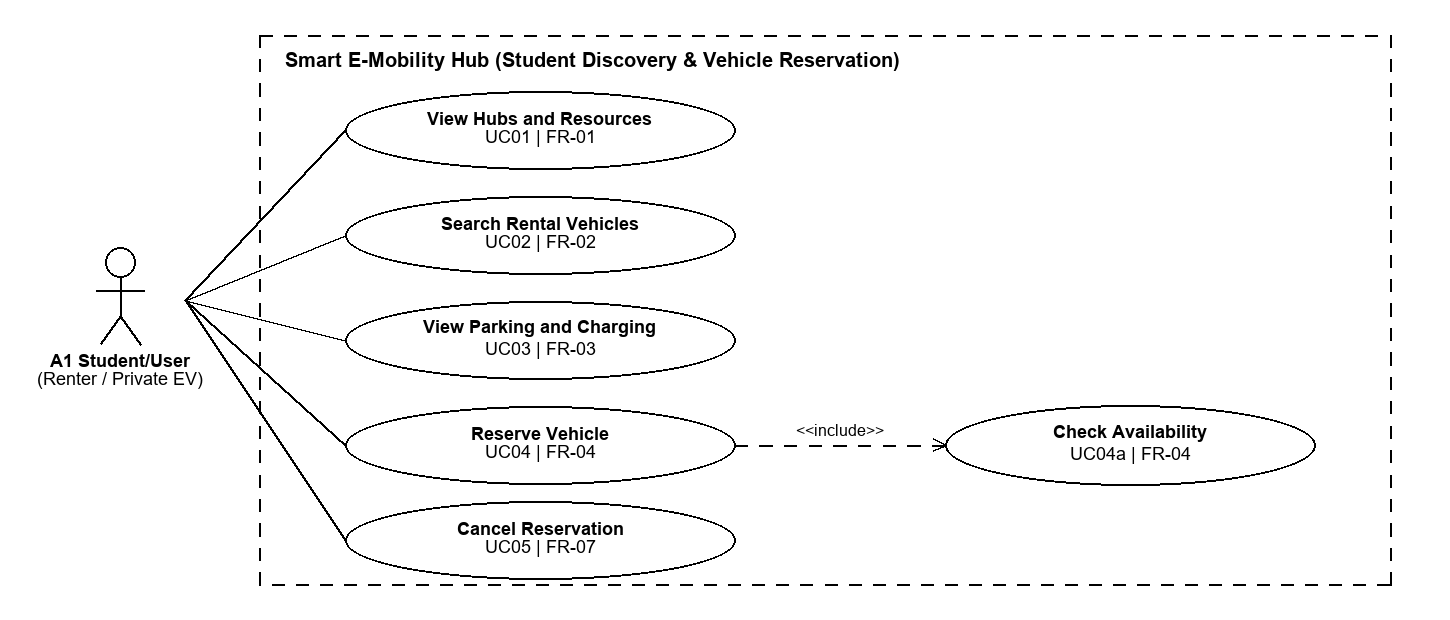
\includegraphics[width=0.88\linewidth]{graphics/diagrams/fig2_1_uc_student_search.png}
  \caption{Use-Case Diagram 1 --- Student: Hub Discovery, Vehicle Search \& Reservation (\texttt{UC01}--\texttt{UC05, UC04a})}
  \label{fig:uc-s1}
\end{figure}

\begin{figure}[H]
  \centering
  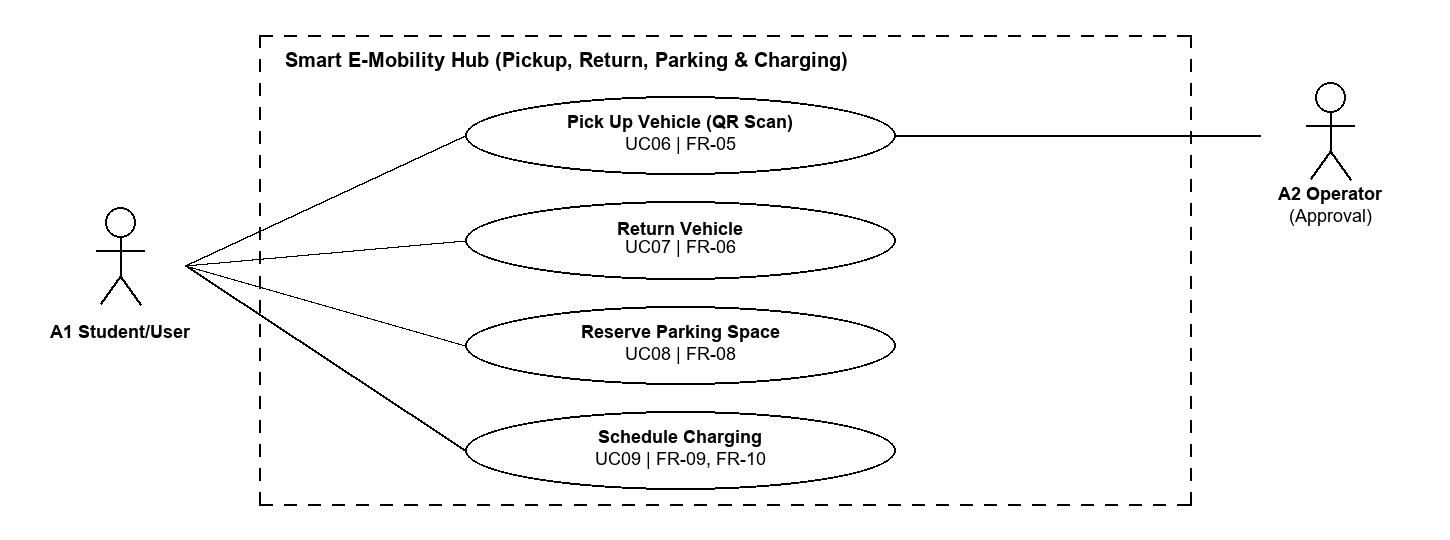
\includegraphics[width=0.88\linewidth]{graphics/diagrams/fig2_2_uc_student_ops.png}
  \caption{Use-Case Diagram 2 --- Student: QR Pickup, Return, Parking \& Smart Charging (\texttt{UC06}--\texttt{UC09})}
  \label{fig:uc-s2}
\end{figure}

\begin{figure}[H]
  \centering
  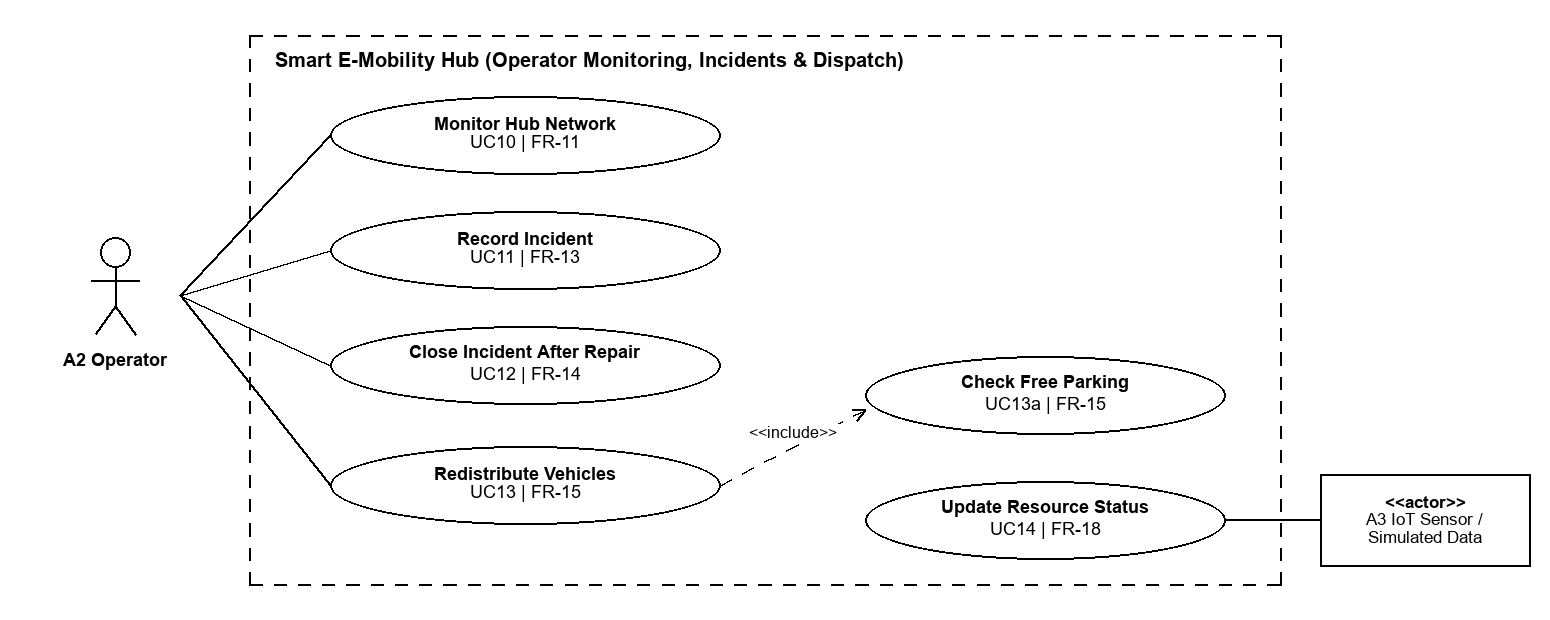
\includegraphics[width=0.90\linewidth]{graphics/diagrams/fig2_3_uc_operator_ops.png}
  \caption{Use-Case Diagram 3 --- Operator: Monitoring, Incidents, Dispatch \& Telemetry (\texttt{UC10}--\texttt{UC14, UC13a})}
  \label{fig:uc-op1}
\end{figure}

\begin{figure}[H]
  \centering
  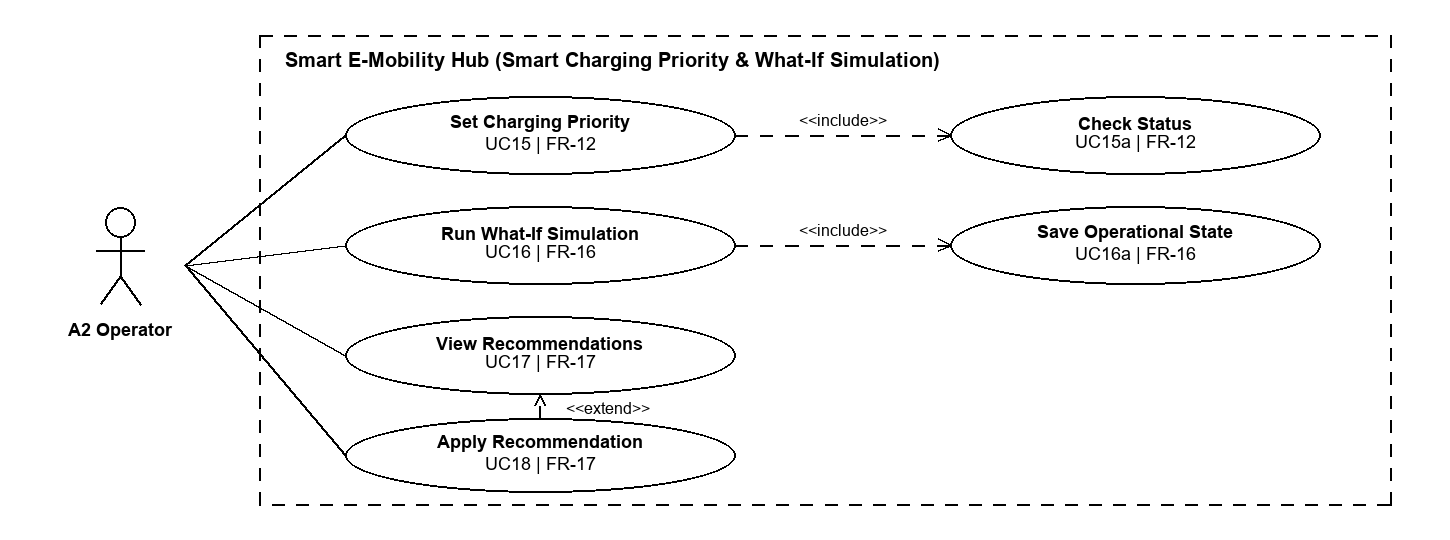
\includegraphics[width=0.88\linewidth]{graphics/diagrams/fig2_4_uc_operator_sim.png}
  \caption{Use-Case Diagram 4 --- Operator: Smart Charging Priority \& What-If Simulation (\texttt{UC15}--\texttt{UC18})}
  \label{fig:uc-op2}
\end{figure}

\safesubsection{Detailed Use-Case Specifications}
\label{subsec:use-case-specs}
\textbf{Actors and Authentication Precondition:} System actors comprise \textbf{A1 User} (specialized by \textbf{A1a Student/Renter} and \textbf{A1b Private EV Owner}), \textbf{A2 Operator}, and \textbf{A3 IoT Sensor / Simulated Data Source}. Users authenticate via campus/email credentials (with pre-configured \texttt{OPERATOR} accounts and default \texttt{USER} accounts for renters/private EV owners); authentication is a universal precondition of every use case rather than a separate domain use case. \Cref{tab:uc-catalog} indexes all 22 use cases and included sub-flows, followed by complete individual specifications in \Cref{tab:uc01,tab:uc02,tab:uc03,tab:uc04,tab:uc04a,tab:uc05,tab:uc06,tab:uc07,tab:uc08,tab:uc09,tab:uc10,tab:uc11,tab:uc12,tab:uc13,tab:uc13a,tab:uc14,tab:uc15,tab:uc15a,tab:uc16,tab:uc16a,tab:uc17,tab:uc18}.

\begin{table}[H]
  \centering
  \singlespacing\footnotesize
  \caption{Master Use-Case Catalog (\texttt{UC01}--\texttt{UC18} and Included Use Cases)}
  \label{tab:uc-catalog}
  \renewcommand{\arraystretch}{1.14}
  \begin{tabularx}{\textwidth}{|C{1.5cm}|Y|C{2.1cm}|L{2.8cm}|}
    \hline
    \rowcolor{tblHeader}
    \textbf{ID} & \textbf{Use Case} & \textbf{Actor} & \textbf{Related FR} \\
    \hline
    \texttt{UC01} & View Hubs and resources & \texttt{A1} & \texttt{FR-01} \\
    \hline
    \texttt{UC02} & Search rental vehicles & \texttt{A1} & \texttt{FR-02} \\
    \hline
    \texttt{UC03} & View parking and charging & \texttt{A1} & \texttt{FR-03} \\
    \hline
    \texttt{UC04} & Reserve vehicle & \texttt{A1} & \texttt{FR-04, FR-05} \\
    \hline
    \texttt{UC04a} & Check availability (included in \texttt{UC04}) & System & \texttt{FR-04} \\
    \hline
    \texttt{UC05} & Cancel reservation & \texttt{A1} & \texttt{FR-07} \\
    \hline
    \texttt{UC06} & Pick up vehicle & \texttt{A1} & \texttt{FR-05} \\
    \hline
    \texttt{UC07} & Return vehicle & \texttt{A1} & \texttt{FR-06} \\
    \hline
    \texttt{UC08} & Reserve parking space & \texttt{A1} & \texttt{FR-08} \\
    \hline
    \texttt{UC09} & Schedule charging & \texttt{A1} & \texttt{FR-09, FR-10} \\
    \hline
    \texttt{UC10} & Monitor Hub network & \texttt{A2} & \texttt{FR-11} \\
    \hline
    \texttt{UC11} & Record incident & \texttt{A2} & \texttt{FR-13} \\
    \hline
    \texttt{UC12} & Close incident after repair & \texttt{A2} & \texttt{FR-14} \\
    \hline
    \texttt{UC13} & Redistribute vehicles & \texttt{A2} & \texttt{FR-15} \\
    \hline
    \texttt{UC13a} & Check free parking (included in \texttt{UC13}) & System & \texttt{FR-15} \\
    \hline
    \texttt{UC14} & Update resource status & \texttt{A3} & \texttt{FR-18} \\
    \hline
    \texttt{UC15} & Set charging priority & \texttt{A2} & \texttt{FR-12} \\
    \hline
    \texttt{UC15a} & Check status (included in \texttt{UC15}) & System & \texttt{FR-12} \\
    \hline
    \texttt{UC16} & Run What-if simulation & \texttt{A2} & \texttt{FR-16} \\
    \hline
    \texttt{UC16a} & Save operational state (included in \texttt{UC16}) & System & \texttt{FR-16} \\
    \hline
    \texttt{UC17} & View recommendations & \texttt{A2} & \texttt{FR-17} \\
    \hline
    \texttt{UC18} & Apply recommendation (extends \texttt{UC17}) & \texttt{A2} & \texttt{FR-17} \\
    \hline
  \end{tabularx}
\end{table}

% --- PAIR 1: UC01 & UC02 ---
\begin{table}[H]
  \centering
  \singlespacing\footnotesize
  \caption{Use-Case Specification --- \texttt{UC01}: View Hubs and Resources}
  \label{tab:uc01}
  \renewcommand{\arraystretch}{1.13}
  \begin{tabularx}{\textwidth}{|L{2.9cm}|Y|}
    \hline
    \rowcolor{tblHeader}
    \textbf{Use-case name} & \textbf{\texttt{UC01} --- View Hubs and resources} \\
    \hline
    \textbf{Actor} & \texttt{A1} Student/User \\
    \hline
    \textbf{Description} & \texttt{A1} views each Mobility Hub on the interactive map and card list with its available rental vehicles, free parking spaces, and available charging points. \\
    \hline
    \textbf{Preconditions} & \texttt{A1} is logged in. Hub status data has been received from \texttt{A3} / live database. \\
    \hline
    \textbf{Normal Flow} & 1.\ \texttt{A1} opens the Hub list or live OpenStreetMap view.\newline
    2.\ System retrieves the current state of all four VNU-HCM Hubs.\newline
    3.\ System computes availability: available vehicles (excluding reserved, \texttt{IN\_\allowbreak USE}, low-battery charging, or \texttt{OUT\_\allowbreak OF\_\allowbreak SERVICE}); free parking $= \text{capacity} - (\text{occupied} + \text{overlapping reserved})$; available chargers $= \text{capacity} - (\text{occupied, reserved, or unavailable})$.\newline
    4.\ System displays each Hub with its saturation badge, name, and the three resource counts.\newline
    5.\ \texttt{A1} selects a Hub marker or card; 6.\ System displays detailed fleet, bay, and charger data for that Hub. \\
    \hline
    \textbf{Exceptions} & \textbf{2a.} Hub telemetry has not updated for $>30\text{ s}$: System displays the last known valid state (with last-update timestamp) and continues at step 3. \\
    \hline
    \textbf{Alternative Flows} & \textbf{5a.} \texttt{A1} does not select a specific Hub: the use case ends after step 4. \\
    \hline
    \textbf{Postconditions} & No state change. \\
    \hline
    \textbf{Related FR / NFR} & \texttt{FR-01}; \texttt{NFR-01, NFR-07} \\
    \hline
  \end{tabularx}
\end{table}

\begin{table}[H]
  \centering
  \singlespacing\footnotesize
  \caption{Use-Case Specification --- \texttt{UC02}: Search Rental Vehicles}
  \label{tab:uc02}
  \renewcommand{\arraystretch}{1.13}
  \begin{tabularx}{\textwidth}{|L{2.9cm}|Y|}
    \hline
    \rowcolor{tblHeader}
    \textbf{Use-case name} & \textbf{\texttt{UC02} --- Search rental vehicles} \\
    \hline
    \textbf{Actor} & \texttt{A1a} Student/User (rental mode) \\
    \hline
    \textbf{Description} & \texttt{A1a} searches shared e-bicycles and e-scooters by Hub, vehicle type, and operational battery/range eligibility. \\
    \hline
    \textbf{Preconditions} & \texttt{A1a} is logged in and browsing shared rental mode. \\
    \hline
    \textbf{Normal Flow} & 1.\ \texttt{A1a} opens the Hub/vehicle search and fleet filter strip.\newline
    2.\ \texttt{A1a} selects filters (Hub keyword, \texttt{Electric bike} / \texttt{Electric scooter}, battery threshold).\newline
    3.\ System queries vehicles in state \texttt{AVAILABLE} whose battery meets the safety threshold ($\text{SoC} \ge 20\%$, \texttt{BR-02}).\newline
    4.\ System displays matching vehicles with availability, current battery percentage, estimated range (km), and VND rate.\newline
    5.\ \texttt{A1a} selects a vehicle to inspect details and may proceed to \texttt{UC04}. \\
    \hline
    \textbf{Exceptions} & \textbf{2a.} Battery filter outside $0\text{--}100\%$: System rejects input with validation feedback; return to step 2.\newline
    \textbf{3a.} No vehicle matches: System shows ``No available vehicles match'' and suggests relaxing filters or trying another Hub. \\
    \hline
    \textbf{Alternative Flows} & \textbf{2b.} \texttt{A1a} leaves optional filters empty: System applies only active filters and shows all eligible vehicles with range estimates; continue step 3. \\
    \hline
    \textbf{Postconditions} & No state change. \\
    \hline
    \textbf{Related FR / NFR} & \texttt{FR-02}; \texttt{BR-02} \\
    \hline
  \end{tabularx}
\end{table}

% --- PAIR 2: UC03 & UC04 ---
\begin{table}[H]
  \centering
  \singlespacing\footnotesize
  \caption{Use-Case Specification --- \texttt{UC03}: View Parking and Charging}
  \label{tab:uc03}
  \renewcommand{\arraystretch}{1.13}
  \begin{tabularx}{\textwidth}{|L{2.9cm}|Y|}
    \hline
    \rowcolor{tblHeader}
    \textbf{Use-case name} & \textbf{\texttt{UC03} --- View parking and charging} \\
    \hline
    \textbf{Actor} & \texttt{A1b} Student/User (private-vehicle mode) \\
    \hline
    \textbf{Description} & \texttt{A1b}, riding a personal EV, views Zone C parking and charging availability and manages isolated personal EV details without invoking shared-rental actions. \\
    \hline
    \textbf{Preconditions} & \texttt{A1b} is logged in and opens Hub Services / Book Parking \& Charger mode. \\
    \hline
    \textbf{Normal Flow} & 1.\ \texttt{A1b} selects a Hub in the private-EV parking/charging workspace (and optionally edits personal EV plate/model).\newline
    2.\ System isolates the view from shared fleet rental holds.\newline
    3.\ System retrieves Zone C (\texttt{PRIVATE\_\allowbreak EV}/\texttt{UNIVERSAL}) parking bays and operational charging points of the Hub.\newline
    4.\ System displays free parking spaces, available chargers, and 7-day hourly availability; 5.\ \texttt{A1b} may continue with \texttt{UC08} or \texttt{UC09}. \\
    \hline
    \textbf{Exceptions} & \textbf{3a.} Telemetry is delayed: System shows last valid counts; continue step 4.\newline
    \textbf{4a.} Zero free parking bays and zero free chargers: System shows full status and suggests nearby VNU-HCM Hubs. \\
    \hline
    \textbf{Alternative Flows} & \textbf{5a.} \texttt{A1b} switches to compare another Hub: return to step 1. \\
    \hline
    \textbf{Postconditions} & No shared-fleet state change (personal EV profile saved per user if edited). \\
    \hline
    \textbf{Related FR / NFR} & \texttt{FR-03}; \texttt{BR-04} \\
    \hline
  \end{tabularx}
\end{table}

\begin{table}[H]
  \centering
  \singlespacing\footnotesize
  \caption{Use-Case Specification --- \texttt{UC04}: Reserve Vehicle}
  \label{tab:uc04}
  \renewcommand{\arraystretch}{1.13}
  \begin{tabularx}{\textwidth}{|L{2.9cm}|Y|}
    \hline
    \rowcolor{tblHeader}
    \textbf{Use-case name} & \textbf{\texttt{UC04} --- Reserve vehicle} \\
    \hline
    \textbf{Actor} & \texttt{A1a} Student/User (primary); \texttt{A2} Operator (booking approval) \\
    \hline
    \textbf{Description} & \texttt{A1a} reserves a shared EV for a 7-day time window at a Hub (including \texttt{UC04a} Check availability), followed by \texttt{A2} approval into a 15-minute pickup hold. \\
    \hline
    \textbf{Preconditions} & \texttt{A1a} is logged in. An eligible vehicle ($\text{SoC} \ge 20\%$) was selected through \texttt{UC02}. \\
    \hline
    \textbf{Normal Flow} & 1.\ \texttt{A1a} selects a vehicle and chooses \textit{Reserve} with a start/end window.\newline
    2.\ System locks \texttt{users} (\texttt{FOR UPDATE}) and checks \texttt{A1a} holds no other open vehicle booking (\texttt{BR-01}).\newline
    3.\ System executes \texttt{UC04a} Check availability under row lock.\newline
    4.\ System creates reservation (\texttt{PENDING}) and holds the vehicle; upon \texttt{A2} clicking \textit{Approve}, status transitions to \texttt{CONFIRMED} and starts the 15-minute pickup deadline timer.\newline
    5.\ System displays confirmation (vehicle, Hub, time window, VND estimate, pickup deadline) and auto-syncs within $4\text{ s}$. \\
    \hline
    \textbf{Exceptions} & \textbf{2a.} \texttt{A1a} already holds an open rental: rejected (\texttt{409 USER\_\allowbreak HAS\_\allowbreak ACTIVE\_\allowbreak RENTAL}); \texttt{A1a} may cancel via \texttt{UC05}.\newline
    \textbf{3a.} \texttt{UC04a} returns invalid (low battery or overlap) or concurrent request locked the EV first: rejected (\texttt{409}); return to step 1/2.\newline
    \textbf{4a.} \texttt{A2} rejects request: reservation becomes \texttt{CANCELLED} (\texttt{OPERATOR\_\allowbreak REJECTED}) and EV returns to \texttt{AVAILABLE}. \\
    \hline
    \textbf{Alternative Flows} & None. \\
    \hline
    \textbf{Postconditions} & Reservation is recorded and the vehicle cannot be double-booked for the overlapping window. \\
    \hline
    \textbf{Related FR / NFR} & \texttt{FR-04, FR-05}; \texttt{NFR-03} \\
    \hline
  \end{tabularx}
\end{table}

% --- PAIR 3: UC04a & UC05 ---
\begin{table}[H]
  \centering
  \singlespacing\footnotesize
  \caption{Use-Case Specification --- \texttt{UC04a}: Check Availability (Included in \texttt{UC04})}
  \label{tab:uc04a}
  \renewcommand{\arraystretch}{1.13}
  \begin{tabularx}{\textwidth}{|L{2.9cm}|Y|}
    \hline
    \rowcolor{tblHeader}
    \textbf{Use-case name} & \textbf{\texttt{UC04a} --- Check availability (included in \texttt{UC04})} \\
    \hline
    \textbf{Actor} & System (no external actor) \\
    \hline
    \textbf{Description} & Verifies transactionally that the selected vehicle remains operational, adequately charged, and free of overlapping bookings for the requested window. \\
    \hline
    \textbf{Preconditions} & \texttt{UC04} has supplied a validated vehicle ID and $[t_{\text{start}}, t_{\text{end}})$ window. \\
    \hline
    \textbf{Normal Flow} & 1.\ System locks and reads the current \texttt{vehicles} row and active \texttt{reservations}.\newline
    2.\ System verifies the Hub is not \texttt{MAINTENANCE}, vehicle is \texttt{AVAILABLE}, and $\text{battery\_level} \ge 20\%$.\newline
    3.\ System verifies $[t_{\text{start}}, t_{\text{end}})$ overlaps zero \texttt{PENDING}, \texttt{CONFIRMED}, or \texttt{ACTIVE} reservations of that vehicle.\newline
    4.\ System returns \texttt{valid} to \texttt{UC04}. \\
    \hline
    \textbf{Exceptions} & \textbf{2a, 3a.} Any check fails: System returns \texttt{invalid} with the exact error code (\texttt{BATTERY\_\allowbreak TOO\_\allowbreak LOW} or \texttt{VEHICLE\_\allowbreak TIME\_\allowbreak SLOT\_\allowbreak BOOKED}) to \texttt{UC04}, which aborts creation. \\
    \hline
    \textbf{Alternative Flows} & None. \\
    \hline
    \textbf{Postconditions} & No state change within \texttt{UC04a} itself. \\
    \hline
    \textbf{Related FR / NFR} & \texttt{FR-04}; \texttt{NFR-03} \\
    \hline
  \end{tabularx}
\end{table}

\begin{table}[H]
  \centering
  \singlespacing\footnotesize
  \caption{Use-Case Specification --- \texttt{UC05}: Cancel Reservation}
  \label{tab:uc05}
  \renewcommand{\arraystretch}{1.13}
  \begin{tabularx}{\textwidth}{|L{2.9cm}|Y|}
    \hline
    \rowcolor{tblHeader}
    \textbf{Use-case name} & \textbf{\texttt{UC05} --- Cancel reservation} \\
    \hline
    \textbf{Actor} & \texttt{A1} Student/User (or System timer on hold expiry) \\
    \hline
    \textbf{Description} & \texttt{A1} cancels a vehicle or parking reservation before pickup/check-in, or the system automatically releases a reservation when the 15-minute pickup hold expires. \\
    \hline
    \textbf{Preconditions} & Reservation is in \texttt{PENDING} or \texttt{CONFIRMED} state and has not been picked up. \\
    \hline
    \textbf{Normal Flow} & 1.\ \texttt{A1} opens the active reservation and selects \textit{Cancel}.\newline
    2.\ System prompts for confirmation; 3.\ \texttt{A1} confirms cancellation.\newline
    4.\ System sets reservation status to \texttt{CANCELLED} with role-safe student attribution (\texttt{STUDENT\_\allowbreak CANCELLED} or \texttt{STUDENT\_\allowbreak DECLINED}, never \texttt{OPERATOR\_\allowbreak REJECTED}) and restores any held vehicle/slot to \texttt{AVAILABLE}/\texttt{FREE}.\newline
    5.\ System displays the updated cancellation badge. \\
    \hline
    \textbf{Exceptions} & \textbf{2a.} Reservation is already \texttt{ACTIVE} (picked up), \texttt{COMPLETED}, or \texttt{EXPIRED}: System rejects cancellation (\texttt{409 INVALID\_\allowbreak STATE\_\allowbreak TRANSITION}) with reason. \\
    \hline
    \textbf{Alternative Flows} & \textbf{3a.} \texttt{A1} dismisses confirmation: no state change; use case ends.\newline
    \textbf{1a (Expiry):} No pickup occurs within 15 minutes after the scheduled start; system marks reservation \texttt{EXPIRED}, restores EV to \texttt{AVAILABLE}, and updates \texttt{A1}'s view. \\
    \hline
    \textbf{Postconditions} & Held vehicle or bay is \texttt{AVAILABLE}/\texttt{FREE} again for other campus users. \\
    \hline
    \textbf{Related FR / NFR} & \texttt{FR-07}; \texttt{BR-03} \\
    \hline
  \end{tabularx}
\end{table}

% --- PAIR 4: UC06 & UC07 ---
\begin{table}[H]
  \centering
  \singlespacing\footnotesize
  \caption{Use-Case Specification --- \texttt{UC06}: Pick Up Vehicle}
  \label{tab:uc06}
  \renewcommand{\arraystretch}{1.13}
  \begin{tabularx}{\textwidth}{|L{2.9cm}|Y|}
    \hline
    \rowcolor{tblHeader}
    \textbf{Use-case name} & \textbf{\texttt{UC06} --- Pick up vehicle} \\
    \hline
    \textbf{Actor} & \texttt{A1a} Student/User \\
    \hline
    \textbf{Description} & \texttt{A1a} unlocks and confirms pickup of an operator-approved vehicle at the designated Hub via optical QR scan. \\
    \hline
    \textbf{Preconditions} & Reservation is \texttt{CONFIRMED} for this \texttt{A1a}, not expired, and \texttt{A1a} is at the designated Hub rack. \\
    \hline
    \textbf{Normal Flow} & 1.\ \texttt{A1a} opens Pickup \& Return, launches the Optical QR Scanner, and scans/confirms the vehicle QR code.\newline
    2.\ System validates the Hub, ownership, non-expiry, and \texttt{CONFIRMED} state.\newline
    3.\ System sets reservation to \texttt{ACTIVE}, sets vehicle to \texttt{IN\_\allowbreak USE}, vacates the origin parking slot to \texttt{FREE}, and recalculates Hub status.\newline
    4.\ System starts the live elapsed ride timer and displays active trip telemetry. \\
    \hline
    \textbf{Exceptions} & \textbf{2a.} Reservation is still \texttt{PENDING}: rejected (\texttt{409 AWAITING\_\allowbreak OPERATOR\_\allowbreak APPROVAL}).\newline
    \textbf{2b.} Reservation expired, cancelled, wrong Hub, or owned by another user: rejected (\texttt{403/409}) with specific reason; \texttt{A1a} may start \texttt{UC02}. \\
    \hline
    \textbf{Alternative Flows} & None. \\
    \hline
    \textbf{Postconditions} & Vehicle is \texttt{IN\_\allowbreak USE}, origin slot is \texttt{FREE}, and hold expiry timer stops. \\
    \hline
    \textbf{Related FR / NFR} & \texttt{FR-05}; \texttt{NFR-03, NFR-07} \\
    \hline
  \end{tabularx}
\end{table}

\begin{table}[H]
  \centering
  \singlespacing\footnotesize
  \caption{Use-Case Specification --- \texttt{UC07}: Return Vehicle}
  \label{tab:uc07}
  \renewcommand{\arraystretch}{1.13}
  \begin{tabularx}{\textwidth}{|L{2.9cm}|Y|}
    \hline
    \rowcolor{tblHeader}
    \textbf{Use-case name} & \textbf{\texttt{UC07} --- Return vehicle} \\
    \hline
    \textbf{Actor} & \texttt{A1a} Student/User \\
    \hline
    \textbf{Description} & \texttt{A1a} returns an active rental EV at a chosen Hub; the system verifies free bay capacity, docks the EV, and updates its post-trip state from battery SoC. \\
    \hline
    \textbf{Preconditions} & Reservation is \texttt{ACTIVE} (picked up) and the vehicle is \texttt{IN\_\allowbreak USE}. \\
    \hline
    \textbf{Normal Flow} & 1.\ \texttt{A1a} selects \textit{Return vehicle} and chooses a destination Hub.\newline
    2.\ System locks destination Hub slots and checks for $\ge 1$ \texttt{FREE} \texttt{SHARED\_\allowbreak EV} or \texttt{UNIVERSAL} parking bay.\newline
    3.\ System evaluates post-trip battery SoC and docks the vehicle into the free bay (\texttt{OCCUPIED}, occupancy $+1$).\newline
    4.\ System closes the reservation as \texttt{COMPLETED} and sets the vehicle to \texttt{AVAILABLE} if $\text{SoC} \ge 20\%$, otherwise flags it for hub charging.\newline
    5.\ System syncs Hub saturation and displays the completed ride \& VND fee summary. \\
    \hline
    \textbf{Exceptions} & \textbf{2a.} Destination Hub is \texttt{MAINTENANCE} or has $0$ free compatible bays: rejected (\texttt{409 RETURN\_\allowbreak HUB\_\allowbreak FULL}); \texttt{A1a} selects another Hub with free capacity (return to step 1). \\
    \hline
    \textbf{Alternative Flows} & \textbf{5a.} Low post-trip SoC triggers charging request workflow (\texttt{UC09}). \\
    \hline
    \textbf{Postconditions} & Reservation is \texttt{COMPLETED} and vehicle is docked at the destination Hub. \\
    \hline
    \textbf{Related FR / NFR} & \texttt{FR-06}; \texttt{BR-02, BR-06} \\
    \hline
  \end{tabularx}
\end{table}

% --- PAIR 5: UC08 & UC09 ---
\begin{table}[H]
  \centering
  \singlespacing\footnotesize
  \caption{Use-Case Specification --- \texttt{UC08}: Reserve Parking Space}
  \label{tab:uc08}
  \renewcommand{\arraystretch}{1.13}
  \begin{tabularx}{\textwidth}{|L{2.9cm}|Y|}
    \hline
    \rowcolor{tblHeader}
    \textbf{Use-case name} & \textbf{\texttt{UC08} --- Reserve parking space} \\
    \hline
    \textbf{Actor} & \texttt{A1} Student/User (private-vehicle or customer parking mode) \\
    \hline
    \textbf{Description} & \texttt{A1} reserves a Zone C (\texttt{PRIVATE\_\allowbreak EV} / \texttt{UNIVERSAL}) parking space at a Hub for a requested time interval. \\
    \hline
    \textbf{Preconditions} & \texttt{A1} is logged in and has selected an operational Hub (\texttt{UC01} or \texttt{UC03}). \\
    \hline
    \textbf{Normal Flow} & 1.\ \texttt{A1} selects a Hub, time interval, and default \texttt{AUTO} free-space mode (or specific bay).\newline
    2.\ System locks compatible Zone C slots and overlapping reservations, computing free spaces $= \text{total} - (\text{occupied} + \text{overlapping active reservations})$.\newline
    3.\ System assigns a free compatible bay, creates the parking reservation, and reduces free capacity for that interval.\newline
    4.\ System displays the booking status and assigned bay code. \\
    \hline
    \textbf{Exceptions} & \textbf{2a.} Free spaces $\le 0$: System rejects (\texttt{409 NO\_\allowbreak PARKING\_\allowbreak AVAILABLE}) and suggests other Hubs or unshaded hours.\newline
    \textbf{3a.} Concurrent request took the last compatible bay: rejected (\texttt{409}) cleanly. \\
    \hline
    \textbf{Alternative Flows} & \textbf{2b.} After a full-interval rejection, \texttt{A1} picks an alternative time window; continue step 2. \\
    \hline
    \textbf{Postconditions} & A conflict-free Zone C parking reservation exists for the interval. \\
    \hline
    \textbf{Related FR / NFR} & \texttt{FR-08}; \texttt{NFR-03, BR-04} \\
    \hline
  \end{tabularx}
\end{table}

\begin{table}[H]
  \centering
  \singlespacing\footnotesize
  \caption{Use-Case Specification --- \texttt{UC09}: Schedule Charging}
  \label{tab:uc09}
  \renewcommand{\arraystretch}{1.13}
  \begin{tabularx}{\textwidth}{|L{2.9cm}|Y|}
    \hline
    \rowcolor{tblHeader}
    \textbf{Use-case name} & \textbf{\texttt{UC09} --- Schedule charging} \\
    \hline
    \textbf{Actor} & \texttt{A1} Student/User (rental or private-vehicle mode) \\
    \hline
    \textbf{Description} & \texttt{A1} requests a $100\%$ target-SoC charging session at a Hub; concurrent requests bind distinct free ports under \texttt{AUTO} mode or enter the Hub waitlist when full. \\
    \hline
    \textbf{Preconditions} & \texttt{A1} is logged in; Hub is operational and vehicle requires charging ($\text{current SoC} < 100\%$). \\
    \hline
    \textbf{Normal Flow} & 1.\ \texttt{A1} selects Hub, vehicle, and time window under default \texttt{AUTO} free-charger mode.\newline
    2.\ System locks Hub \texttt{charging\_\allowbreak points} and overlapping \texttt{charging\_\allowbreak requests} (\texttt{FOR UPDATE}).\newline
    3.\ System selects an operational charger not booked in $[t_{\text{start}}, t_{\text{end}})$ (enabling 2+ students to book the same hour when 2+ ports are free).\newline
    4.\ System locks the port, creates session (\texttt{SCHEDULED}), and displays port code, window, and estimated kWh/VND fee. \\
    \hline
    \textbf{Exceptions} & \textbf{2a.} Hub in \texttt{MAINTENANCE}, vehicle invalid, or target SoC $\neq 100\%$: rejected (\texttt{409/422}) with reason. \\
    \hline
    \textbf{Alternative Flows} & \textbf{3a.} Zero ports free in $[t_{\text{start}}, t_{\text{end}})$: System places the request into the Hub's waiting queue (\texttt{QUEUED}) without preempting locked bookings; assigned when a port frees (\texttt{UC15}). \\
    \hline
    \textbf{Postconditions} & Charging request exists as \texttt{SCHEDULED} or \texttt{QUEUED}; no port is double-booked. \\
    \hline
    \textbf{Related FR / NFR} & \texttt{FR-09, FR-10}; \texttt{NFR-03, BR-05} \\
    \hline
  \end{tabularx}
\end{table}

% --- PAIR 6: UC10 & UC11 ---
\begin{table}[H]
  \centering
  \singlespacing\footnotesize
  \caption{Use-Case Specification --- \texttt{UC10}: Monitor Hub Network}
  \label{tab:uc10}
  \renewcommand{\arraystretch}{1.13}
  \begin{tabularx}{\textwidth}{|L{2.9cm}|Y|}
    \hline
    \rowcolor{tblHeader}
    \textbf{Use-case name} & \textbf{\texttt{UC10} --- Monitor Hub network} \\
    \hline
    \textbf{Actor} & \texttt{A2} Operator \\
    \hline
    \textbf{Description} & \texttt{A2} monitors fleet distribution, 3-zone parking occupancy, charger status, pending approvals, and Hub utilization across the entire VNU-HCM network. \\
    \hline
    \textbf{Preconditions} & \texttt{A2} is authenticated with \texttt{OPERATOR} role. \\
    \hline
    \textbf{Normal Flow} & 1.\ \texttt{A2} opens the Operator Control Console (\textit{Overview} / \textit{Hub utilization}).\newline
    2.\ System retrieves synchronized telemetry across all Hubs simultaneously.\newline
    3.\ System renders 4 KPI cards, live map pins, 3-zone bay occupancy, charger status, and pending approval requests.\newline
    4.\ \texttt{A2} selects a Hub or resource; 5.\ System shows granular slot/unit status and open incidents. \\
    \hline
    \textbf{Exceptions} & \textbf{2a.} Telemetry source delayed $>30\text{ s}$: System retains last valid resource state and logs timestamp; continue step 3. \\
    \hline
    \textbf{Alternative Flows} & \textbf{4a.} \texttt{A2} filters by Hub or zone: view refreshes immediately.\newline
    \textbf{4b.} New status report (\texttt{UC14}) or booking arrives: dashboard auto-refreshes every $10\text{ s}$. \\
    \hline
    \textbf{Postconditions} & No state change (unless \texttt{A2} invokes an approval or check-in action). \\
    \hline
    \textbf{Related FR / NFR} & \texttt{FR-11}; \texttt{NFR-01, NFR-07} \\
    \hline
  \end{tabularx}
\end{table}

\begin{table}[H]
  \centering
  \singlespacing\footnotesize
  \caption{Use-Case Specification --- \texttt{UC11}: Record Incident}
  \label{tab:uc11}
  \renewcommand{\arraystretch}{1.13}
  \begin{tabularx}{\textwidth}{|L{2.9cm}|Y|}
    \hline
    \rowcolor{tblHeader}
    \textbf{Use-case name} & \textbf{\texttt{UC11} --- Record incident} \\
    \hline
    \textbf{Actor} & \texttt{A2} Operator \\
    \hline
    \textbf{Description} & \texttt{A2} logs a hardware/operational fault on a mandatory target vehicle or charging point, immediately isolating it from new bookings. \\
    \hline
    \textbf{Preconditions} & \texttt{A2} is logged in; target resource exists and is not already isolated under the same open fault. \\
    \hline
    \textbf{Normal Flow} & 1.\ \texttt{A2} opens \textit{Incidents}, selects Hub, target type (\texttt{Vehicle} or \texttt{Charging point}), mandatory unit ID, severity, and description.\newline
    2.\ System sets the target resource to \texttt{OUT\_\allowbreak OF\_\allowbreak SERVICE} / \texttt{MAINTENANCE} inside an InnoDB transaction.\newline
    3.\ System immediately blocks new reservations and charging sessions on that unit.\newline
    4.\ System records the incident (\texttt{OPEN}), flags any overlapping upcoming bookings for reassignment, and displays confirmation. \\
    \hline
    \textbf{Exceptions} & \textbf{1a.} No specific target unit selected: rejected (\texttt{400 VALIDATION\_\allowbreak FAILED}).\newline
    \textbf{2a.} Resource is already isolated with an active open incident: system warns \texttt{A2} and displays the existing incident. \\
    \hline
    \textbf{Alternative Flows} & \textbf{4a.} Zero upcoming bookings affected: notification step skipped; \texttt{A2} may trigger \texttt{UC13} if Hub stock drops. \\
    \hline
    \textbf{Postconditions} & Target resource is \texttt{OUT\_\allowbreak OF\_\allowbreak SERVICE} and an open incident persists until \texttt{UC12}. \\
    \hline
    \textbf{Related FR / NFR} & \texttt{FR-13}; \texttt{BR-07} \\
    \hline
  \end{tabularx}
\end{table}

% --- PAIR 7: UC12 & UC13 ---
\begin{table}[H]
  \centering
  \singlespacing\footnotesize
  \caption{Use-Case Specification --- \texttt{UC12}: Close Incident After Repair}
  \label{tab:uc12}
  \renewcommand{\arraystretch}{1.13}
  \begin{tabularx}{\textwidth}{|L{2.9cm}|Y|}
    \hline
    \rowcolor{tblHeader}
    \textbf{Use-case name} & \textbf{\texttt{UC12} --- Close incident after repair} \\
    \hline
    \textbf{Actor} & \texttt{A2} Operator \\
    \hline
    \textbf{Description} & \texttt{A2} resolves an open/assigned incident by recording field repair notes, restoring the isolated vehicle or charger to operational availability. \\
    \hline
    \textbf{Preconditions} & An \texttt{OPEN} or \texttt{IN\_\allowbreak PROGRESS} incident exists and physical repair was completed by field crew (\texttt{S4}). \\
    \hline
    \textbf{Normal Flow} & 1.\ \texttt{A2} selects the incident (optionally clicking \textit{Assign staff} $\rightarrow$ \texttt{IN\_\allowbreak PROGRESS} first) and clicks \textit{Resolve}.\newline
    2.\ \texttt{A2} enters non-empty repair result notes.\newline
    3.\ System validates the repair notes, closes the incident (\texttt{RESOLVED}/\texttt{CLOSED}), and restores the target vehicle or charging point to \texttt{AVAILABLE}.\newline
    4.\ System recalculates Hub capacity and confirms restoration. \\
    \hline
    \textbf{Exceptions} & \textbf{3a.} Repair result note is empty: System rejects closure (\texttt{400}); resource remains \texttt{OUT\_\allowbreak OF\_\allowbreak SERVICE}. \\
    \hline
    \textbf{Alternative Flows} & \textbf{2a.} Field crew reports unit unrepairable: \texttt{A2} keeps incident open and unit remains isolated. \\
    \hline
    \textbf{Postconditions} & Incident is closed and the repaired unit is selectable for new bookings again. \\
    \hline
    \textbf{Related FR / NFR} & \texttt{FR-14}; \texttt{BR-07} \\
    \hline
  \end{tabularx}
\end{table}

\begin{table}[H]
  \centering
  \singlespacing\footnotesize
  \caption{Use-Case Specification --- \texttt{UC13}: Redistribute Vehicles}
  \label{tab:uc13}
  \renewcommand{\arraystretch}{1.13}
  \begin{tabularx}{\textwidth}{|L{2.9cm}|Y|}
    \hline
    \rowcolor{tblHeader}
    \textbf{Use-case name} & \textbf{\texttt{UC13} --- Redistribute vehicles} \\
    \hline
    \textbf{Actor} & \texttt{A2} Operator \\
    \hline
    \textbf{Description} & \texttt{A2} transfers \texttt{AVAILABLE} shared rental EVs slot-to-slot between Hubs (including \texttt{UC13a} Check free parking), excluding private customer EVs. \\
    \hline
    \textbf{Preconditions} & \texttt{A2} is logged in; selected shared EVs are \texttt{AVAILABLE} at the source Hub. \\
    \hline
    \textbf{Normal Flow} & 1.\ \texttt{A2} selects source Hub, destination Hub, assigned staff, and \texttt{AVAILABLE} shared EVs paired to target Zone A / Universal bays (from \textit{Dispatch} or \texttt{UC18}).\newline
    2.\ System runs \texttt{UC13a} Check free parking under row lock.\newline
    3.\ Inside a two-phase transaction, Phase A frees source slots (\texttt{FREE}) and Phase B binds vehicles to destination Hub \& bays (\texttt{OCCUPIED}), logging \texttt{dispatch\_\allowbreak orders}.\newline
    4.\ System updates vehicle counts and saturation statuses of both Hubs simultaneously and confirms completion. \\
    \hline
    \textbf{Exceptions} & \textbf{1a.} Vehicle is reserved, \texttt{IN\_\allowbreak USE}, \texttt{OUT\_\allowbreak OF\_\allowbreak SERVICE}, or a private EV: rejected (\texttt{409/422}).\newline
    \textbf{2a.} \texttt{UC13a} reports destination Hub closed or lacking free bays: rejected (\texttt{409}); return to step 1. \\
    \hline
    \textbf{Alternative Flows} & None. \\
    \hline
    \textbf{Postconditions} & Total network fleet size is conserved; both Hubs reflect updated slot and EV counts. \\
    \hline
    \textbf{Related FR / NFR} & \texttt{FR-15}; \texttt{BR-04, BR-06} \\
    \hline
  \end{tabularx}
\end{table}

% --- PAIR 8: UC13a & UC14 ---
\begin{table}[H]
  \centering
  \singlespacing\footnotesize
  \caption{Use-Case Specification --- \texttt{UC13a}: Check Free Parking (Included in \texttt{UC13})}
  \label{tab:uc13a}
  \renewcommand{\arraystretch}{1.13}
  \begin{tabularx}{\textwidth}{|L{2.9cm}|Y|}
    \hline
    \rowcolor{tblHeader}
    \textbf{Use-case name} & \textbf{\texttt{UC13a} --- Check free parking (included in \texttt{UC13})} \\
    \hline
    \textbf{Actor} & System \\
    \hline
    \textbf{Description} & Verifies transactionally that the destination Hub is operational and has sufficient free \texttt{SHARED\_\allowbreak EV} / \texttt{UNIVERSAL} parking bays for incoming vehicles. \\
    \hline
    \textbf{Preconditions} & \texttt{UC13} has supplied destination Hub ID and transfer quantity / target slots. \\
    \hline
    \textbf{Normal Flow} & 1.\ System locks and reads the destination Hub status, Zone A/C slot states, and overlapping active parking reservations.\newline
    2.\ System computes verified free fleet-compatible bays and checks $\text{free} \ge \text{transfer count}$.\newline
    3.\ System returns \texttt{valid} (and candidate target slots) to \texttt{UC13}. \\
    \hline
    \textbf{Exceptions} & \textbf{2a.} Destination Hub in \texttt{MAINTENANCE} or free bays $<$ transfer count: returns \texttt{invalid} with reason; \texttt{UC13} rolls back. \\
    \hline
    \textbf{Alternative Flows} & None. \\
    \hline
    \textbf{Postconditions} & No state change within \texttt{UC13a}. \\
    \hline
    \textbf{Related FR / NFR} & \texttt{FR-15}; \texttt{NFR-03} \\
    \hline
  \end{tabularx}
\end{table}

\begin{table}[H]
  \centering
  \singlespacing\footnotesize
  \caption{Use-Case Specification --- \texttt{UC14}: Update Resource Status}
  \label{tab:uc14}
  \renewcommand{\arraystretch}{1.13}
  \begin{tabularx}{\textwidth}{|L{2.9cm}|Y|}
    \hline
    \rowcolor{tblHeader}
    \textbf{Use-case name} & \textbf{\texttt{UC14} --- Update resource status} \\
    \hline
    \textbf{Actor} & \texttt{A3} IoT Sensor / Simulated Data Source \\
    \hline
    \textbf{Description} & \texttt{A3} submits a telemetry status report; the system validates payload bounds and updates vehicle SoC, parking-slot state, or charger state. \\
    \hline
    \textbf{Preconditions} & \texttt{A3} client is connected and the referenced resource ID is registered. \\
    \hline
    \textbf{Normal Flow} & 1.\ \texttt{A3} sends a telemetry report (resource ID, resource type, new status/SoC value, ISO-8601 timestamp).\newline
    2.\ System validates completeness, numeric bounds (e.g.\ battery $0\text{--}100\%$), and valid enum transition.\newline
    3.\ System updates the vehicle, parking slot, or charging point record.\newline
    4.\ System recalculates Hub utilization (\texttt{syncHubStatus}) and exposes fresh metrics to \texttt{A2} (\texttt{UC10}). \\
    \hline
    \textbf{Exceptions} & \textbf{2a.} Payload malformed, out of range ($<0\%$ or $>100\%$), or unknown ID: System rejects (\texttt{400/422}), logs error, and preserves the last valid state.\newline
    \textbf{2b.} No report for $>30\text{ s}$: System retains last known valid state with its last-updated timestamp. \\
    \hline
    \textbf{Alternative Flows} & \textbf{2c.} Out-of-order reports arrive for the same unit: System retains the state carrying the latest timestamp. \\
    \hline
    \textbf{Postconditions} & Stored operational state reflects the latest valid telemetry report. \\
    \hline
    \textbf{Related FR / NFR} & \texttt{FR-18}; \texttt{NFR-01, NFR-06} \\
    \hline
  \end{tabularx}
\end{table}

% --- PAIR 9: UC15 & UC15a ---
\begin{table}[H]
  \centering
  \singlespacing\footnotesize
  \caption{Use-Case Specification --- \texttt{UC15}: Set Charging Priority}
  \label{tab:uc15}
  \renewcommand{\arraystretch}{1.13}
  \begin{tabularx}{\textwidth}{|L{2.9cm}|Y|}
    \hline
    \rowcolor{tblHeader}
    \textbf{Use-case name} & \textbf{\texttt{UC15} --- Set charging priority} \\
    \hline
    \textbf{Actor} & \texttt{A2} Operator \\
    \hline
    \textbf{Description} & \texttt{A2} sets priority levels on waiting charging sessions (including \texttt{UC15a} Check status) and assigns/swaps free charging points to the highest-priority EVs first. \\
    \hline
    \textbf{Preconditions} & \texttt{A2} is logged in; Hub has waiting charging requests (\texttt{QUEUED}) or active ports. \\
    \hline
    \textbf{Normal Flow} & 1.\ \texttt{A2} opens the 2-table \textit{Vehicle \& charging} console.\newline
    2.\ System runs \texttt{UC15a} Check status and renders Table 1 (Active Chargers) alongside Table 2 (Priority Waitlist).\newline
    3.\ \texttt{A2} updates session priority (\texttt{URGENT}, \texttt{HIGH}, \texttt{NORMAL}, \texttt{LOW}) based on battery criticality or expected demand.\newline
    4.\ System persists the priority, re-sorts the queue overriding FIFO, and binds free ports (or executes \texttt{Plug-in}/\texttt{Swap}/\texttt{Unplug}) to top-priority sessions.\newline
    5.\ System displays confirmation and updated charger bindings. \\
    \hline
    \textbf{Exceptions} & \textbf{2a.} Queue is empty: System displays empty waitlist state; use case ends.\newline
    \textbf{4a.} Zero ports currently free: Updated priority order is saved and applied as soon as a port is unplugged. \\
    \hline
    \textbf{Alternative Flows} & \textbf{3a.} Priority update is invoked automatically from a confirmed simulation recommendation (\texttt{UC18}). \\
    \hline
    \textbf{Postconditions} & Waiting sessions are ordered strictly by priority (\texttt{URGENT..LOW}, then FIFO) and free ports are assigned. \\
    \hline
    \textbf{Related FR / NFR} & \texttt{FR-12}; \texttt{BR-05} \\
    \hline
  \end{tabularx}
\end{table}

\begin{table}[H]
  \centering
  \singlespacing\footnotesize
  \caption{Use-Case Specification --- \texttt{UC15a}: Check Status (Included in \texttt{UC15})}
  \label{tab:uc15a}
  \renewcommand{\arraystretch}{1.13}
  \begin{tabularx}{\textwidth}{|L{2.9cm}|Y|}
    \hline
    \rowcolor{tblHeader}
    \textbf{Use-case name} & \textbf{\texttt{UC15a} --- Check status (included in \texttt{UC15})} \\
    \hline
    \textbf{Actor} & System \\
    \hline
    \textbf{Description} & Collects live charging-point states and queued vehicle battery/priority metrics required for smart charger assignment. \\
    \hline
    \textbf{Preconditions} & \texttt{UC15} has requested charging state for a Hub or the network. \\
    \hline
    \textbf{Normal Flow} & 1.\ System reads Hub charging points (\texttt{AVAILABLE}, \texttt{OCCUPIED}, \texttt{RESERVED}, \texttt{OUT\_\allowbreak OF\_\allowbreak SERVICE}).\newline
    2.\ System reads \texttt{QUEUED} charging requests along with current EV battery SoC, priority enum, and arrival timestamp.\newline
    3.\ System returns the consolidated dataset to \texttt{UC15}. \\
    \hline
    \textbf{Exceptions} & \textbf{1a.} A charging point is \texttt{OUT\_\allowbreak OF\_\allowbreak SERVICE} or stale: System excludes it from automatic assignment. \\
    \hline
    \textbf{Alternative Flows} & None. \\
    \hline
    \textbf{Postconditions} & No state change. \\
    \hline
    \textbf{Related FR / NFR} & \texttt{FR-12} \\
    \hline
  \end{tabularx}
\end{table}

% --- PAIR 10: UC16 & UC16a ---
\begin{table}[H]
  \centering
  \singlespacing\footnotesize
  \caption{Use-Case Specification --- \texttt{UC16}: Run What-If Simulation}
  \label{tab:uc16}
  \renewcommand{\arraystretch}{1.13}
  \begin{tabularx}{\textwidth}{|L{2.9cm}|Y|}
    \hline
    \rowcolor{tblHeader}
    \textbf{Use-case name} & \textbf{\texttt{UC16} --- Run What-if simulation} \\
    \hline
    \textbf{Actor} & \texttt{A2} Operator \\
    \hline
    \textbf{Description} & \texttt{A2} executes a hypothetical stress scenario on an isolated RAM copy of live state (including \texttt{UC16a} Save operational state) without altering live MySQL data. \\
    \hline
    \textbf{Preconditions} & \texttt{A2} is logged in; live operational state is readable. \\
    \hline
    \textbf{Normal Flow} & 1.\ \texttt{A2} opens \textit{What-if} and selects a scenario (demand surge, Hub full, charging surge, partial charger failure, or vehicle concentration).\newline
    2.\ \texttt{A2} enters parameters (target Hub, magnitude, duration, seed); 3.\ System validates parameter ranges.\newline
    4.\ System runs \texttt{UC16a} Save operational state to obtain a deep-cloned sandbox snapshot.\newline
    5.\ System steps discrete 1-minute simulated time on the copy and computes impact indicators (\texttt{I1}--\texttt{I8}).\newline
    6.\ System displays simulated metrics and generates ranked recommendations (\texttt{UC17}). \\
    \hline
    \textbf{Exceptions} & \textbf{3a.} Out-of-range parameters: rejected (\texttt{400}); return to step 2.\newline
    \textbf{5a.} Simulation fails or exceeds the $30\text{ s}$ cap: System aborts, discards the RAM copy, and leaves live data untouched. \\
    \hline
    \textbf{Alternative Flows} & \textbf{6a.} \texttt{A2} adjusts scenario parameters and re-runs; return to step 2. \\
    \hline
    \textbf{Postconditions} & Live reservations, EV locations, and charging sessions experience $0$ database writes. \\
    \hline
    \textbf{Related FR / NFR} & \texttt{FR-16}; \texttt{NFR-02, NFR-04} \\
    \hline
  \end{tabularx}
\end{table}

\begin{table}[H]
  \centering
  \singlespacing\footnotesize
  \caption{Use-Case Specification --- \texttt{UC16a}: Save Operational State (Included in \texttt{UC16})}
  \label{tab:uc16a}
  \renewcommand{\arraystretch}{1.13}
  \begin{tabularx}{\textwidth}{|L{2.9cm}|Y|}
    \hline
    \rowcolor{tblHeader}
    \textbf{Use-case name} & \textbf{\texttt{UC16a} --- Save operational state (included in \texttt{UC16})} \\
    \hline
    \textbf{Actor} & System \\
    \hline
    \textbf{Description} & Builds an isolated in-memory deep copy of live operational tables as the immutable starting baseline for What-If simulation. \\
    \hline
    \textbf{Preconditions} & \texttt{UC16} has validated scenario input parameters. \\
    \hline
    \textbf{Normal Flow} & 1.\ System reads a consistent snapshot of \texttt{hubs}, \texttt{vehicles}, \texttt{parking\_\allowbreak slots}, \texttt{charging\_\allowbreak points}, \texttt{reservations}, and \texttt{charging\_\allowbreak requests}.\newline
    2.\ System deep-clones the object graph in memory tagged as sandbox simulation state.\newline
    3.\ System returns the isolated snapshot to \texttt{UC16}. \\
    \hline
    \textbf{Exceptions} & \textbf{1a.} Snapshot read error: System aborts \texttt{UC16} cleanly and reports error to \texttt{A2}. \\
    \hline
    \textbf{Alternative Flows} & None. \\
    \hline
    \textbf{Postconditions} & Isolated memory snapshot exists; live MySQL tables remain untouched. \\
    \hline
    \textbf{Related FR / NFR} & \texttt{FR-16}; \texttt{NFR-04} \\
    \hline
  \end{tabularx}
\end{table}

% --- PAIR 11: UC17 & UC18 ---
\begin{table}[H]
  \centering
  \singlespacing\footnotesize
  \caption{Use-Case Specification --- \texttt{UC17}: View Recommendations}
  \label{tab:uc17}
  \renewcommand{\arraystretch}{1.13}
  \begin{tabularx}{\textwidth}{|L{2.9cm}|Y|}
    \hline
    \rowcolor{tblHeader}
    \textbf{Use-case name} & \textbf{\texttt{UC17} --- View recommendations} \\
    \hline
    \textbf{Actor} & \texttt{A2} Operator \\
    \hline
    \textbf{Description} & \texttt{A2} inspects ranked coordination recommendations (vehicle redistribution or charging priority promotion) produced by a completed What-If run. \\
    \hline
    \textbf{Preconditions} & A finished simulation result exists from \texttt{UC16}. \\
    \hline
    \textbf{Normal Flow} & 1.\ \texttt{A2} views the recommendation panel of the completed simulation.\newline
    2.\ System lists candidate actions (\texttt{R1}--\texttt{R4}) achieving $\ge 5\%$ composite stress reduction, all marked \texttt{Pending}.\newline
    3.\ \texttt{A2} inspects a recommendation; 4.\ System displays affected Hubs, EV count or queue priority target, and Before vs.\ After impact indicators. \\
    \hline
    \textbf{Exceptions} & \textbf{2a.} No candidate action improves network stress by $\ge 5\%$: System states that no coordination intervention is required. \\
    \hline
    \textbf{Alternative Flows} & \textbf{4a.} \texttt{A2} chooses to execute a recommendation on live state: \texttt{UC18} extends \texttt{UC17}. \\
    \hline
    \textbf{Postconditions} & No live state change; recommendations remain \texttt{Pending}. \\
    \hline
    \textbf{Related FR / NFR} & \texttt{FR-17} \\
    \hline
  \end{tabularx}
\end{table}

\begin{table}[H]
  \centering
  \singlespacing\footnotesize
  \caption{Use-Case Specification --- \texttt{UC18}: Apply Recommendation (Extends \texttt{UC17})}
  \label{tab:uc18}
  \renewcommand{\arraystretch}{1.13}
  \begin{tabularx}{\textwidth}{|L{2.9cm}|Y|}
    \hline
    \rowcolor{tblHeader}
    \textbf{Use-case name} & \textbf{\texttt{UC18} --- Apply recommendation (extends \texttt{UC17})} \\
    \hline
    \textbf{Actor} & \texttt{A2} Operator \\
    \hline
    \textbf{Description} & \texttt{A2} explicitly confirms a \texttt{Pending} recommendation, prompting live-state revalidation and transactional execution via \texttt{UC13} or \texttt{UC15}. \\
    \hline
    \textbf{Preconditions} & A \texttt{Pending} recommendation is selected in \texttt{UC17}. \\
    \hline
    \textbf{Normal Flow} & 1.\ \texttt{A2} clicks \textit{Apply} on the selected recommendation.\newline
    2.\ System displays the concrete live actions to be taken and requests explicit confirmation; 3.\ \texttt{A2} confirms.\newline
    4.\ System revalidates all domain guards against current live MySQL state (free destination bays, charger availability, shared EVs still \texttt{AVAILABLE}).\newline
    5.\ System executes the action transactionally via \texttt{UC13} (redistribution) or \texttt{UC15} (charging priority), marks the recommendation \texttt{Applied}, and displays the result. \\
    \hline
    \textbf{Exceptions} & \textbf{3a.} \texttt{A2} declines confirmation: zero live writes; recommendation stays \texttt{Pending}.\newline
    \textbf{4a.} Live Hub state changed since simulation snapshot causing a rule check to fail: System rejects execution (\texttt{409 STALE\_\allowbreak RECOMMENDATION}) and marks the recommendation outdated. \\
    \hline
    \textbf{Alternative Flows} & None. \\
    \hline
    \textbf{Postconditions} & Only explicitly confirmed and live-revalidated recommendations mutate live operational tables. \\
    \hline
    \textbf{Related FR / NFR} & \texttt{FR-17}; \texttt{NFR-03, NFR-04} \\
    \hline
  \end{tabularx}
\end{table}

\clearpage
\section{Behavioral, Interaction, and User-Interface Design}
\label{sec:behavioral-ui}

\safesubsection{Activity Diagrams}
\label{subsec:activity-diagrams}
System workflows, guard conditions, concurrency checks, and exception branches are modeled using five monochrome UML 2.5 swimlane Activity Diagrams synchronized with the delivered V2.2 platform:
\begin{itemize}
  \item \textbf{Shared EV Rental Lifecycle (\Cref{fig:act-rental}):} Traces hub search, atomic overlap \& battery checks ($\ge 20\%$), \texttt{PENDING} creation, Operator approval (\texttt{CONFIRMED}) vs.\ rejection (\texttt{OPERATOR\_\allowbreak REJECTED}), Student optical QR unlock (\texttt{ACTIVE}) vs.\ cancellation/expiry, and capacity-verified hub return (\texttt{COMPLETED}).
  \item \textbf{Parking \& Multi-Charger Scheduling (\Cref{fig:act-charging}):} Models Zone C customer bay booking and \texttt{AUTO} multi-charger port locking where multiple students receive distinct free ports concurrently until hub capacity saturates into the \texttt{QUEUED} priority waitlist.
  \item \textbf{Incident Isolation \& Recovery (\Cref{fig:act-incident}):} Enforces mandatory affected-unit selection, immediate \texttt{OUT\_\allowbreak OF\_\allowbreak SERVICE} isolation, staff assignment (\texttt{IN\_\allowbreak PROGRESS}), and repair-verified restoration.
  \item \textbf{Two-Phase Redistribution \& Priority Queue (\Cref{fig:act-dispatch}):} Illustrates Phase A source-slot vacation and Phase B destination-slot binding (excluding private EVs), alongside 2-table priority re-ranking and charger swaps.
  \item \textbf{What-If Simulation (\Cref{fig:act-sim}):} Depicts read-only snapshot cloning into RAM, 1-minute discrete evolution, impact scoring (\texttt{I1..I8}), and live-state revalidation prior to applying confirmed actions.
\end{itemize}

\begin{figure}[H]
  \centering
  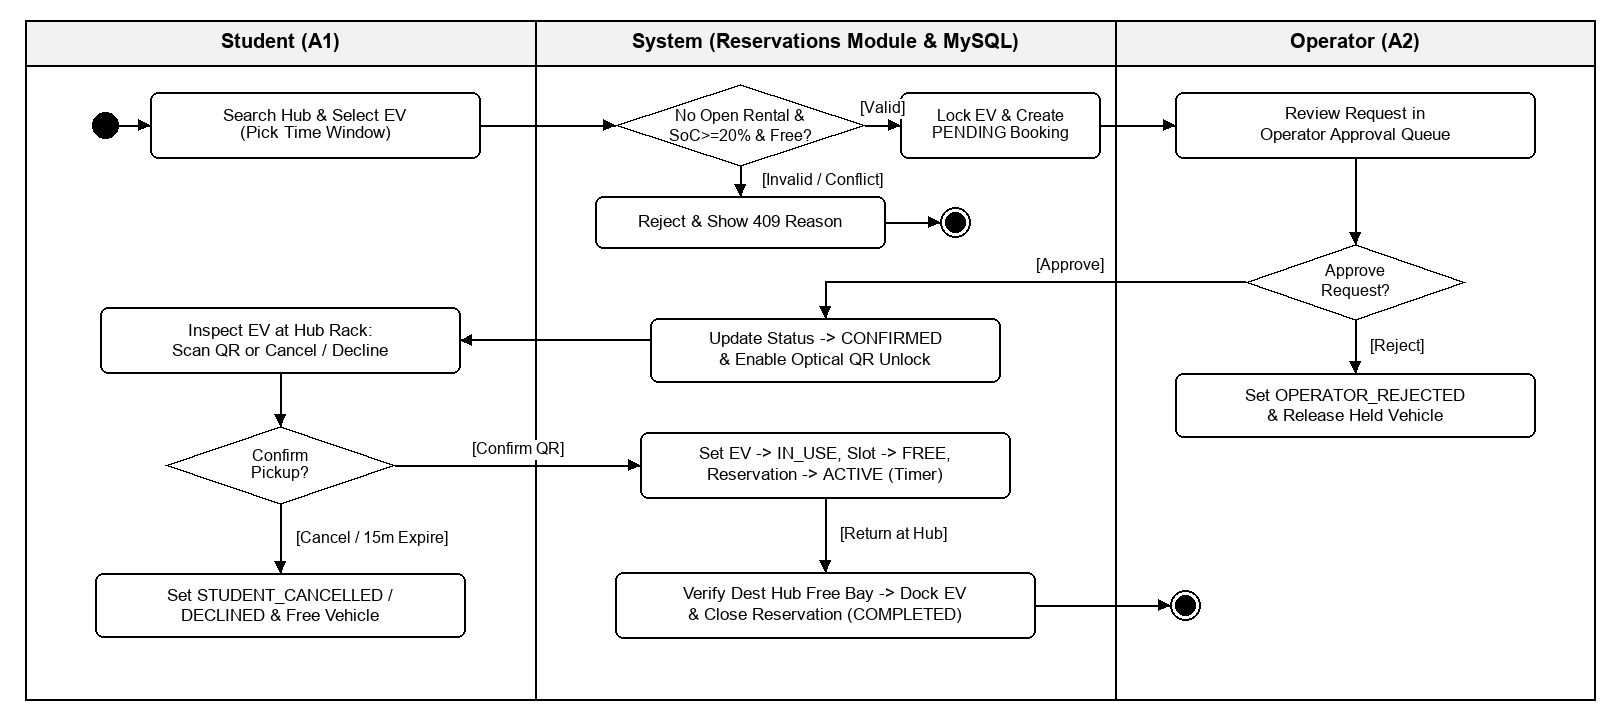
\includegraphics[width=0.92\linewidth]{graphics/diagrams/fig3_1_act_rental.png}
  \caption{Activity Diagram --- 5-Stage Shared EV Reservation, Approval, QR Pickup \& Return}
  \label{fig:act-rental}
\end{figure}

\begin{figure}[H]
  \centering
  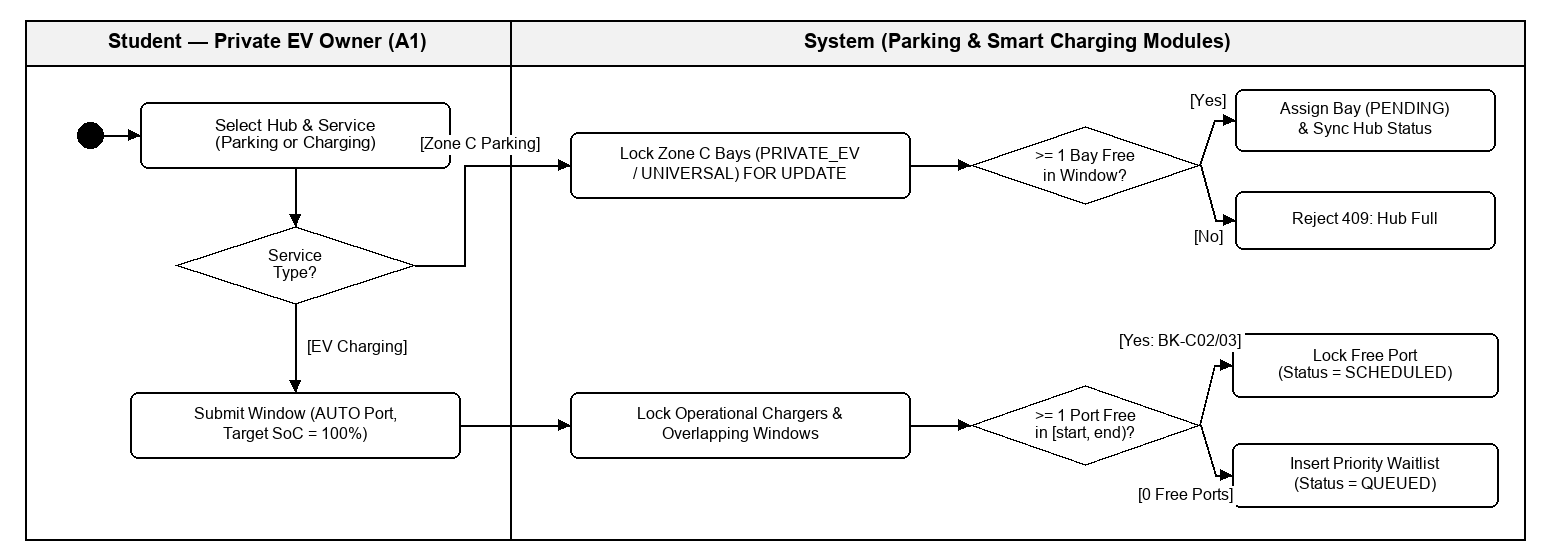
\includegraphics[width=0.90\linewidth]{graphics/diagrams/fig3_2_act_parking_charging.png}
  \caption{Activity Diagram --- Zone C Parking Reservation \& Multi-Charger \texttt{AUTO} Scheduling}
  \label{fig:act-charging}
\end{figure}

\begin{figure}[H]
  \centering
  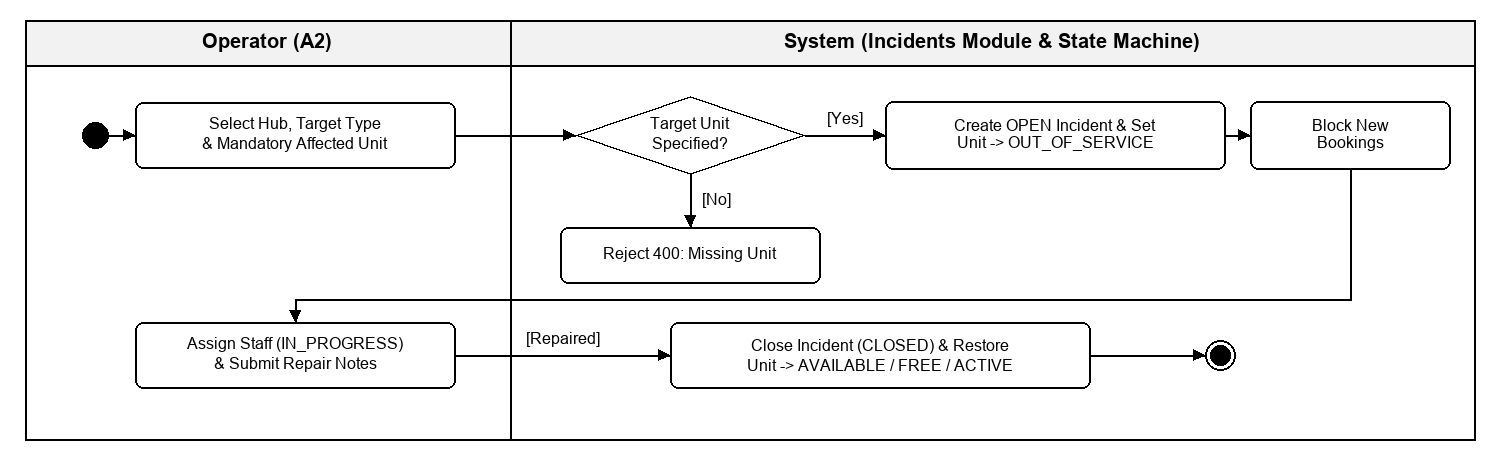
\includegraphics[width=0.90\linewidth]{graphics/diagrams/fig3_3_act_incident.png}
  \caption{Activity Diagram --- Mandatory-Target Incident Isolation \& Repair Resolution}
  \label{fig:act-incident}
\end{figure}

\begin{figure}[H]
  \centering
  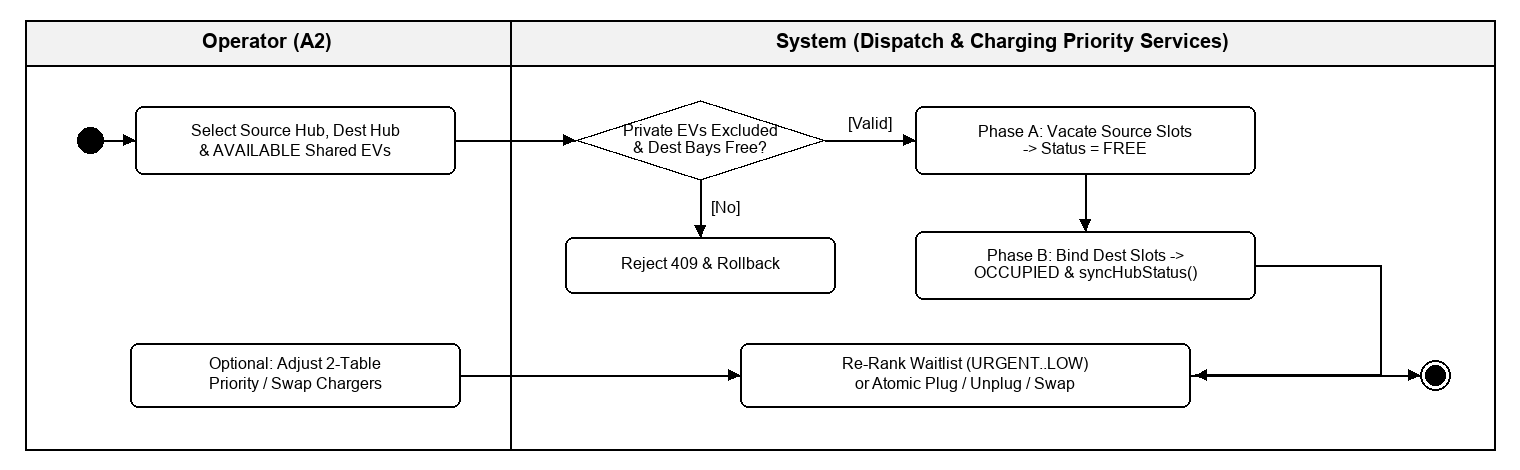
\includegraphics[width=0.90\linewidth]{graphics/diagrams/fig3_4_act_dispatch_priority.png}
  \caption{Activity Diagram --- Two-Phase Slot-to-Slot Vehicle Redistribution \& Charging Priority}
  \label{fig:act-dispatch}
\end{figure}

\begin{figure}[H]
  \centering
  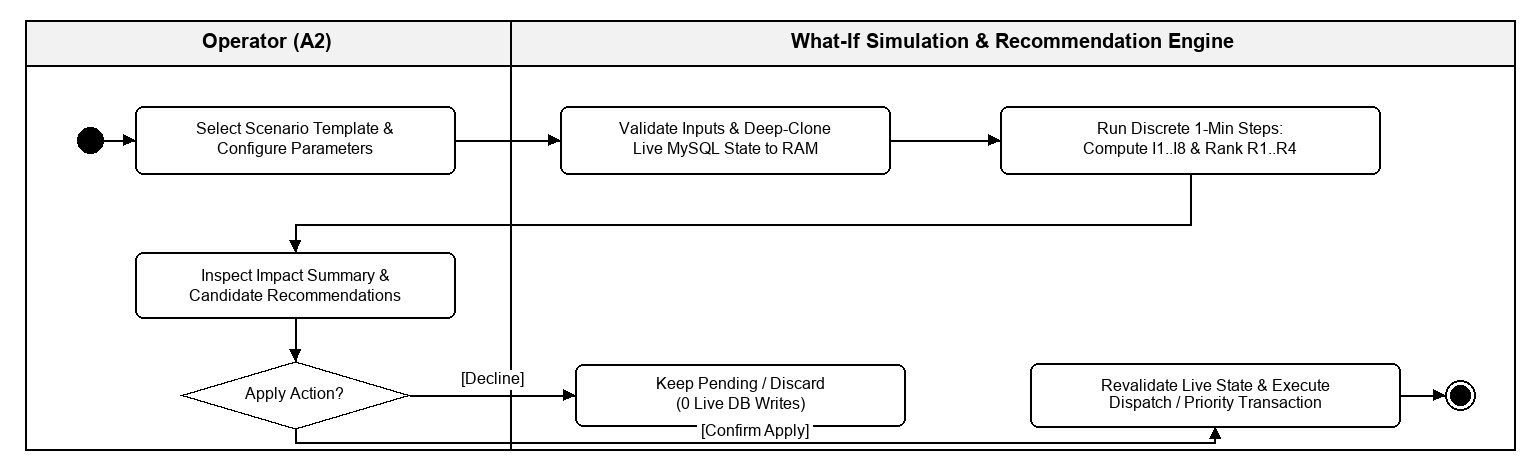
\includegraphics[width=0.90\linewidth]{graphics/diagrams/fig3_5_act_whatif.png}
  \caption{Activity Diagram --- Isolated What-If Simulation \& Live Revalidation}
  \label{fig:act-sim}
\end{figure}

\safesubsection{Sequence Diagrams}
\label{subsec:sequence-diagrams}
Four UML 2.5 Sequence Diagrams formalize chronological message ordering across actors, React UI views, Express REST Controllers, Domain Services, MySQL 8.0 InnoDB transactions, and the In-Memory Sandbox: Shared EV reservation, approval, and QR pickup (\Cref{fig:seq-reserve}); concurrent multi-charger scheduling (\Cref{fig:seq-charging}); two-phase slot-to-slot redistribution (\Cref{fig:seq-dispatch}); and What-If simulation execution (\Cref{fig:seq-sim}).

\begin{figure}[H]
  \centering
  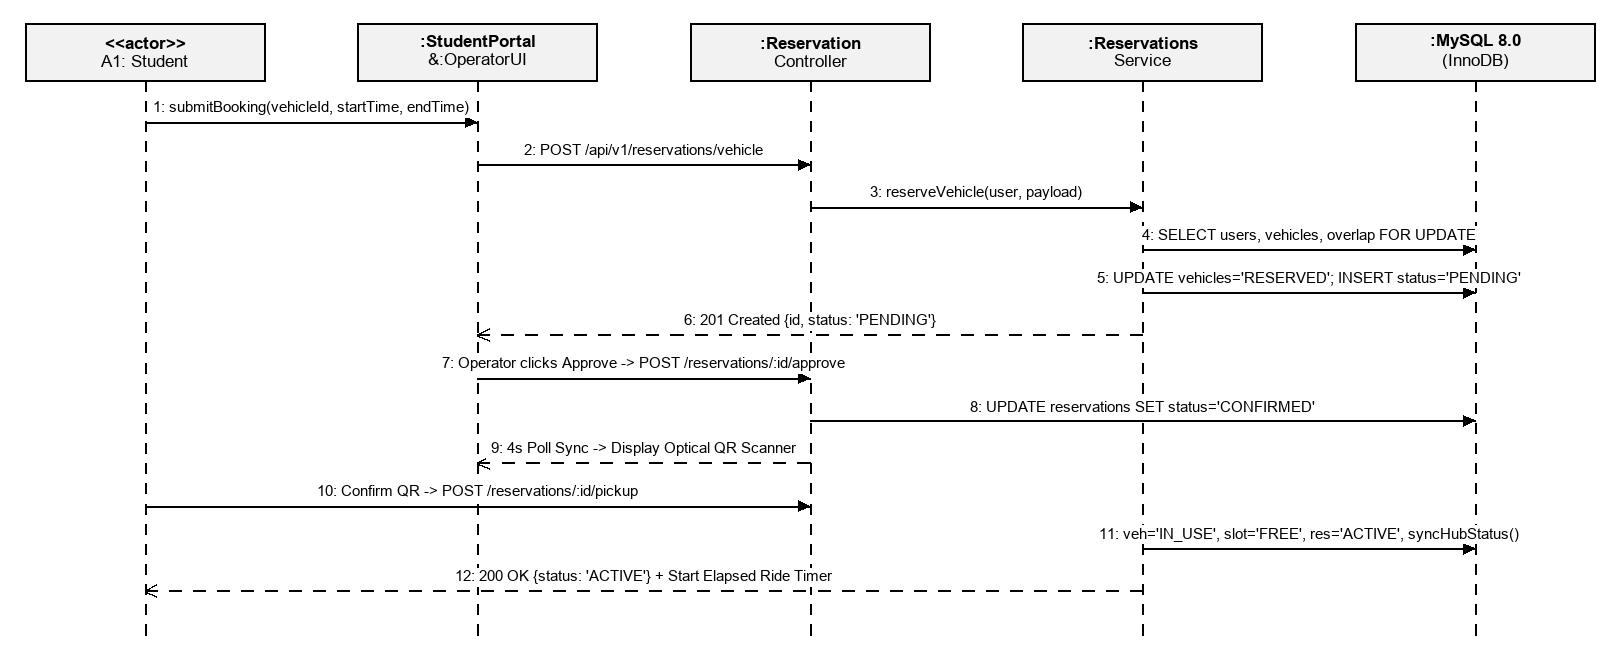
\includegraphics[width=0.92\linewidth]{graphics/diagrams/fig3_6_seq_reserve.png}
  \caption{Sequence Diagram --- Reserve Shared EV, Operator Approval \& Optical QR Pickup}
  \label{fig:seq-reserve}
\end{figure}

\begin{figure}[H]
  \centering
  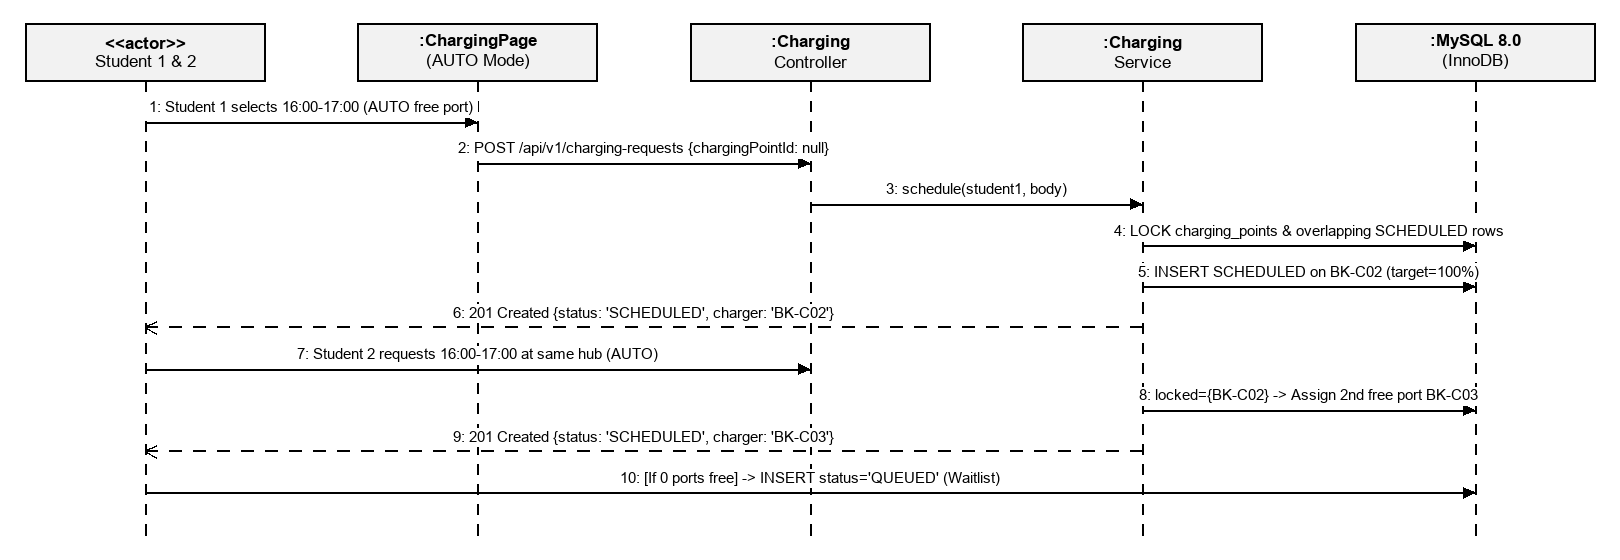
\includegraphics[width=0.92\linewidth]{graphics/diagrams/fig3_7_seq_charging.png}
  \caption{Sequence Diagram --- Concurrent Multi-Charger Scheduling \& Priority Waitlist}
  \label{fig:seq-charging}
\end{figure}

\begin{figure}[H]
  \centering
  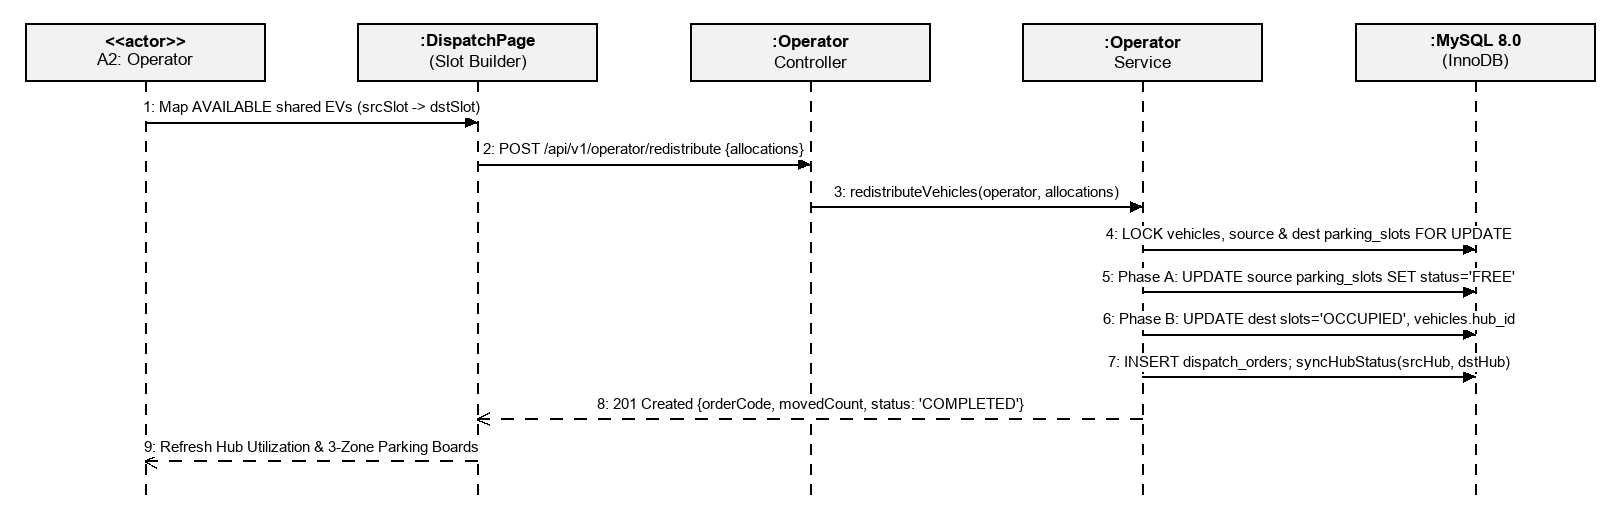
\includegraphics[width=0.92\linewidth]{graphics/diagrams/fig3_8_seq_dispatch.png}
  \caption{Sequence Diagram --- Two-Phase Slot-to-Slot Vehicle Redistribution}
  \label{fig:seq-dispatch}
\end{figure}

\begin{figure}[H]
  \centering
  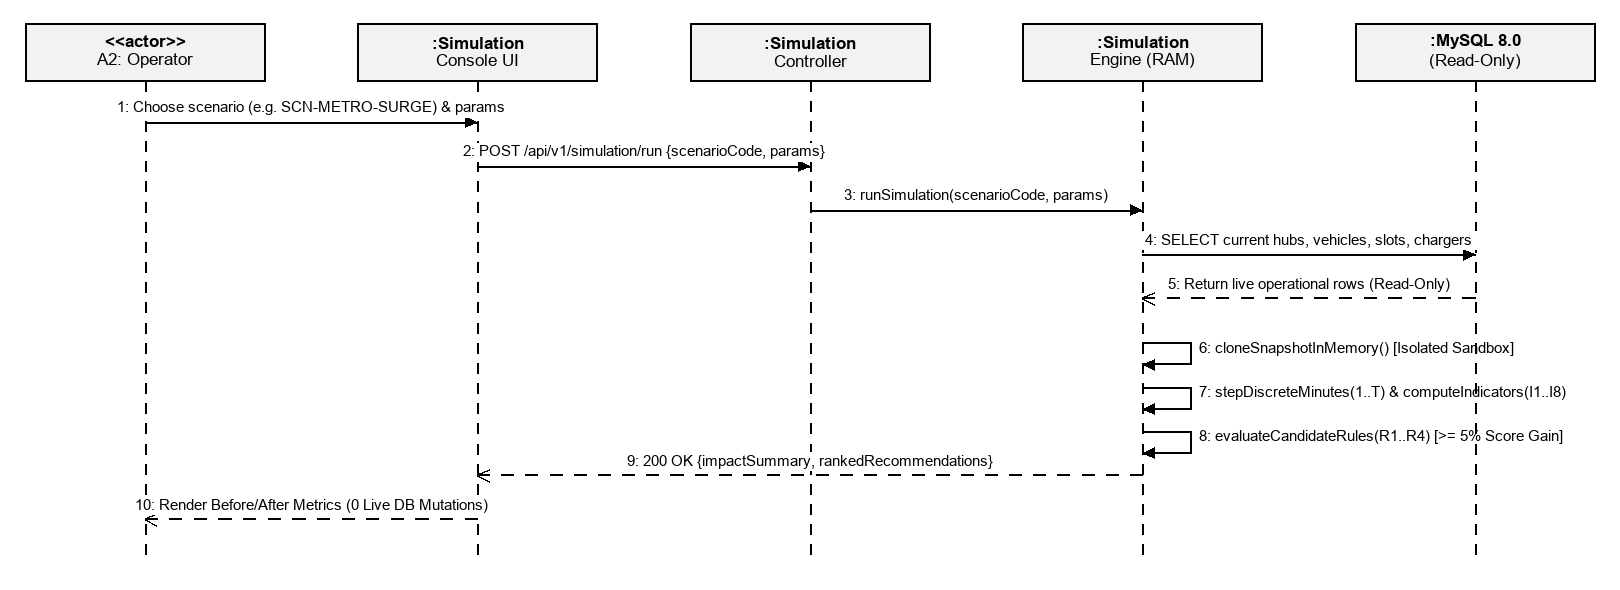
\includegraphics[width=0.92\linewidth]{graphics/diagrams/fig3_9_seq_whatif.png}
  \caption{Sequence Diagram --- Isolated What-If Scenario Execution \& Recommendation Ranking}
  \label{fig:seq-sim}
\end{figure}

\safesubsection{State Machine Diagrams}
\label{subsec:state-machines}
To prevent illegal resource mutations under concurrent operations, explicit state machines govern \texttt{Vehicle} (\Cref{fig:sm-vehicle}), the 5-stage \texttt{Reservation} lifecycle with role-safe cancellation attribution (\Cref{fig:sm-reservation}), and \texttt{ParkingSlot} / \texttt{ChargingPoint} (\Cref{fig:sm-slot-charger}).

\begin{figure}[H]
  \centering
  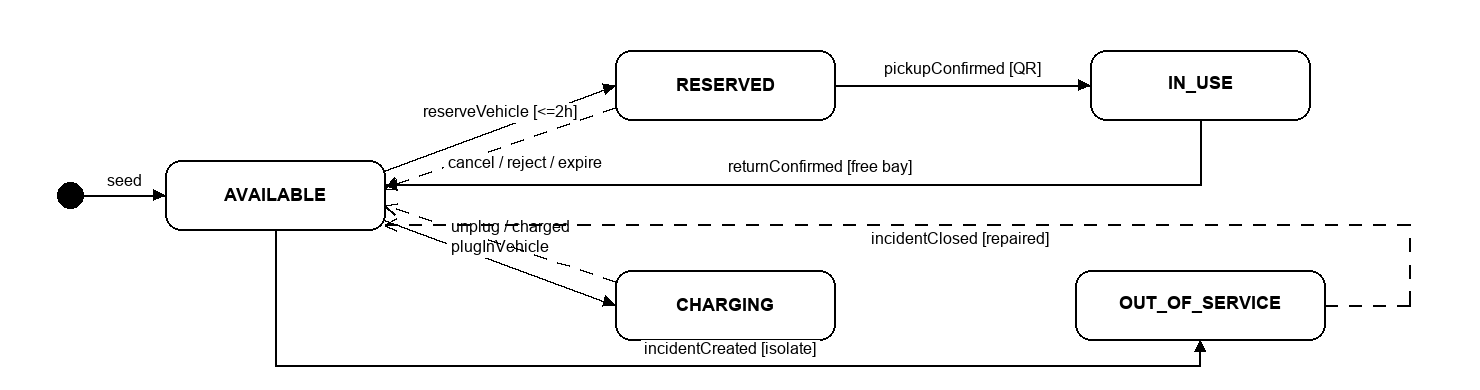
\includegraphics[width=0.90\linewidth]{graphics/diagrams/fig3_10_sm_vehicle.png}
  \caption{State Machine Diagram --- Shared Fleet \texttt{Vehicle} Lifecycle}
  \label{fig:sm-vehicle}
\end{figure}

\begin{figure}[H]
  \centering
  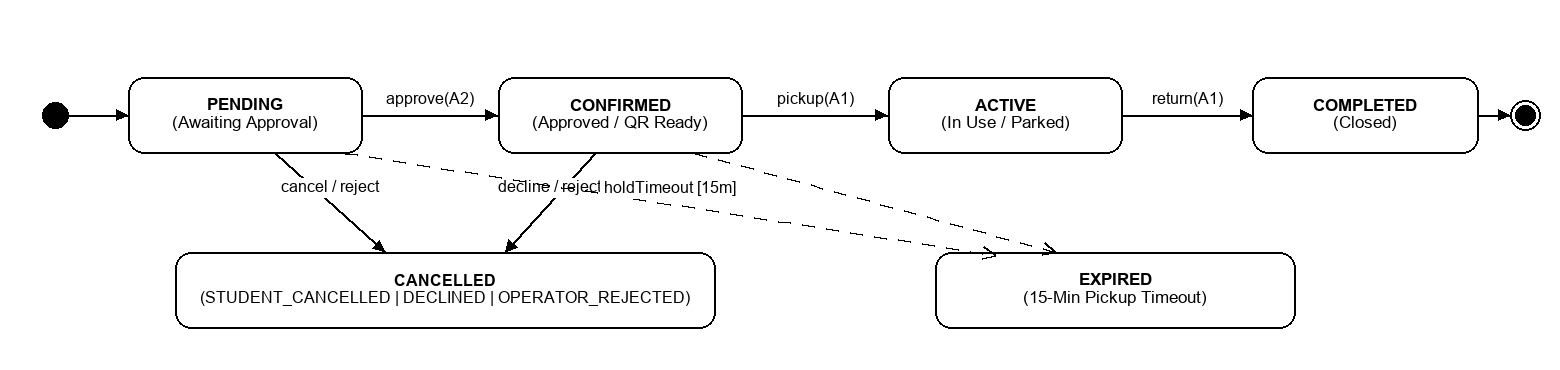
\includegraphics[width=0.92\linewidth]{graphics/diagrams/fig3_11_sm_reservation.png}
  \caption{State Machine Diagram --- 5-Stage \texttt{Reservation} Lifecycle}
  \label{fig:sm-reservation}
\end{figure}

\begin{figure}[H]
  \centering
  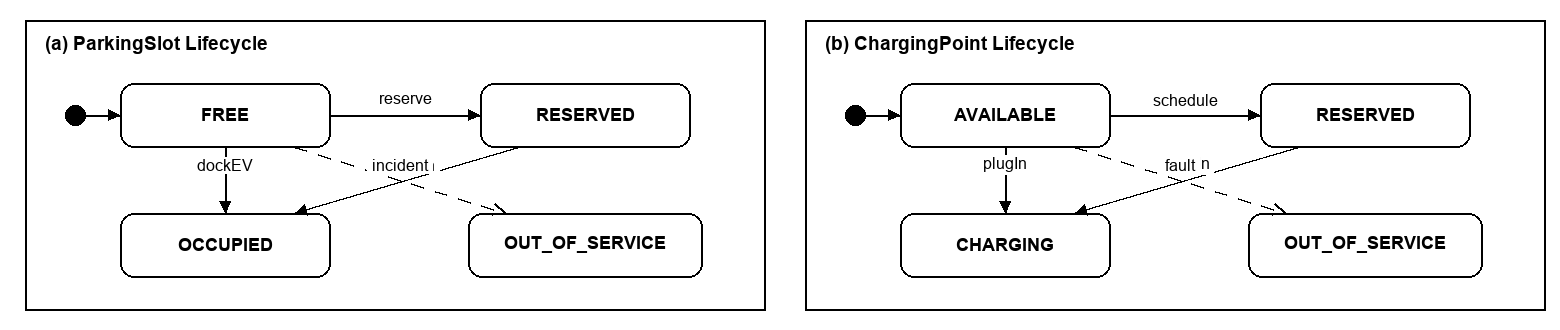
\includegraphics[width=0.92\linewidth]{graphics/diagrams/fig3_12_sm_slot_charger.png}
  \caption{State Machine Diagrams --- \texttt{ParkingSlot} and \texttt{ChargingPoint} Lifecycles}
  \label{fig:sm-slot-charger}
\end{figure}

\safesubsection{User-Interface Design}
\label{subsec:ui-design}
The V2.2 web and mobile interface separates Student (\texttt{USER}) and Staff (\texttt{OPERATOR}) workspaces behind a unified VNU-HCM header featuring Dark/Light mode switching (\Cref{fig:ui-nav}). Following the structural wireframes (\Cref{fig:wf-student,fig:wf-operator}), \Cref{fig:ui-auth,fig:ui-student-map,fig:ui-student-flows,fig:ui-operator-console,fig:ui-operator-ops,fig:ui-mobile-lan} present the delivered V2.2 application screens across authentication, interactive campus hub discovery, 5-stage reservation and \texttt{AUTO} charger scheduling, operator approval and 2-table charging control, incident isolation, slot-to-slot vehicle dispatch, isolated What-If simulation, and responsive Dark-Mode mobile operation over the campus Wi-Fi LAN (\texttt{192.168.1.7:5173}). \Cref{tab:ui-screens} summarizes all screens and feedback mechanisms.

\begin{figure}[H]
  \centering
  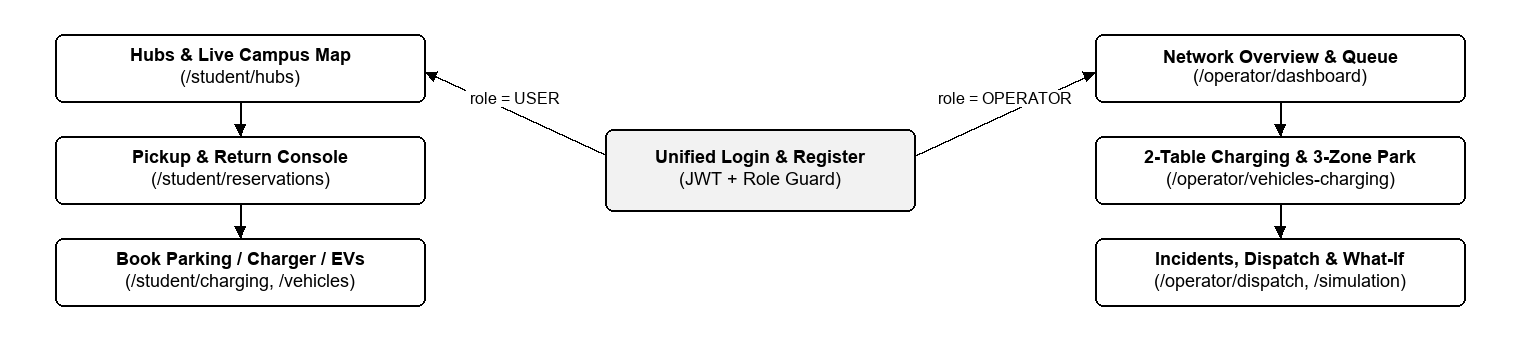
\includegraphics[width=0.90\linewidth]{graphics/diagrams/fig3_13_ui_sitemap.png}
  \caption{Role-Based Navigation Sitemap Across Student Portal and Operator Console}
  \label{fig:ui-nav}
\end{figure}

\begin{figure}[H]
  \centering
  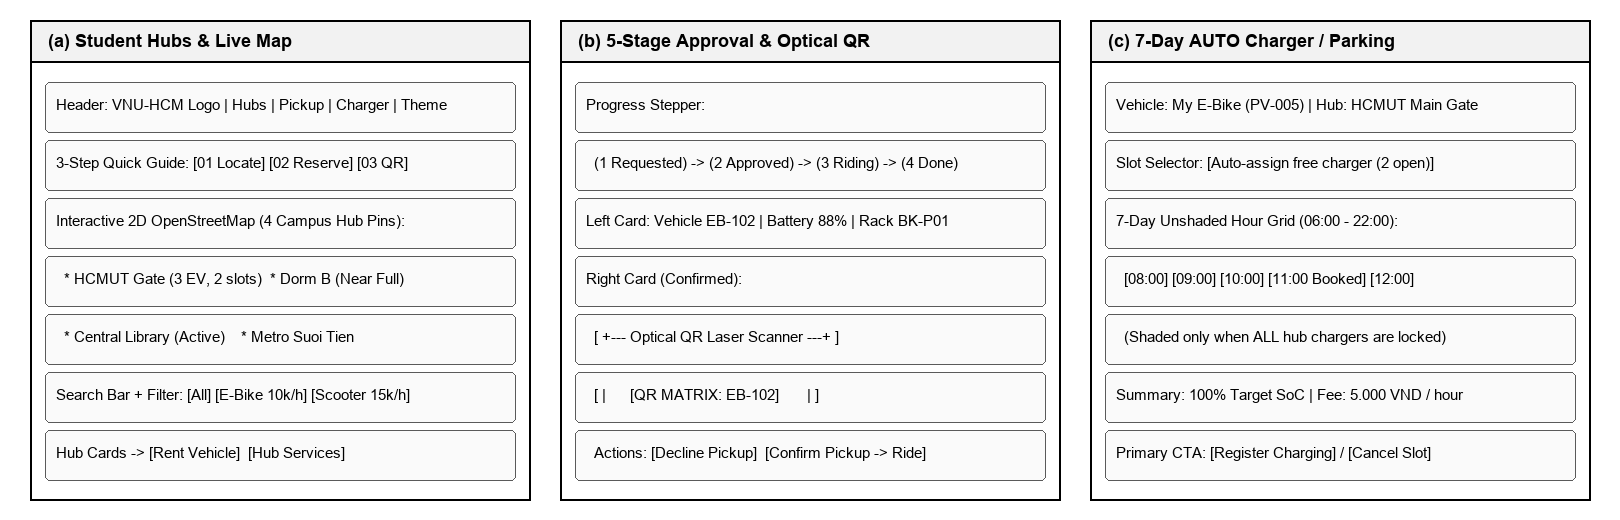
\includegraphics[width=0.94\linewidth]{graphics/diagrams/fig3_14_wf_student.png}
  \caption{Student Portal V2.2 Structural Wireframes (Live Map, QR Scanner, 7-Day \texttt{AUTO} Picker)}
  \label{fig:wf-student}
\end{figure}

\begin{figure}[H]
  \centering
  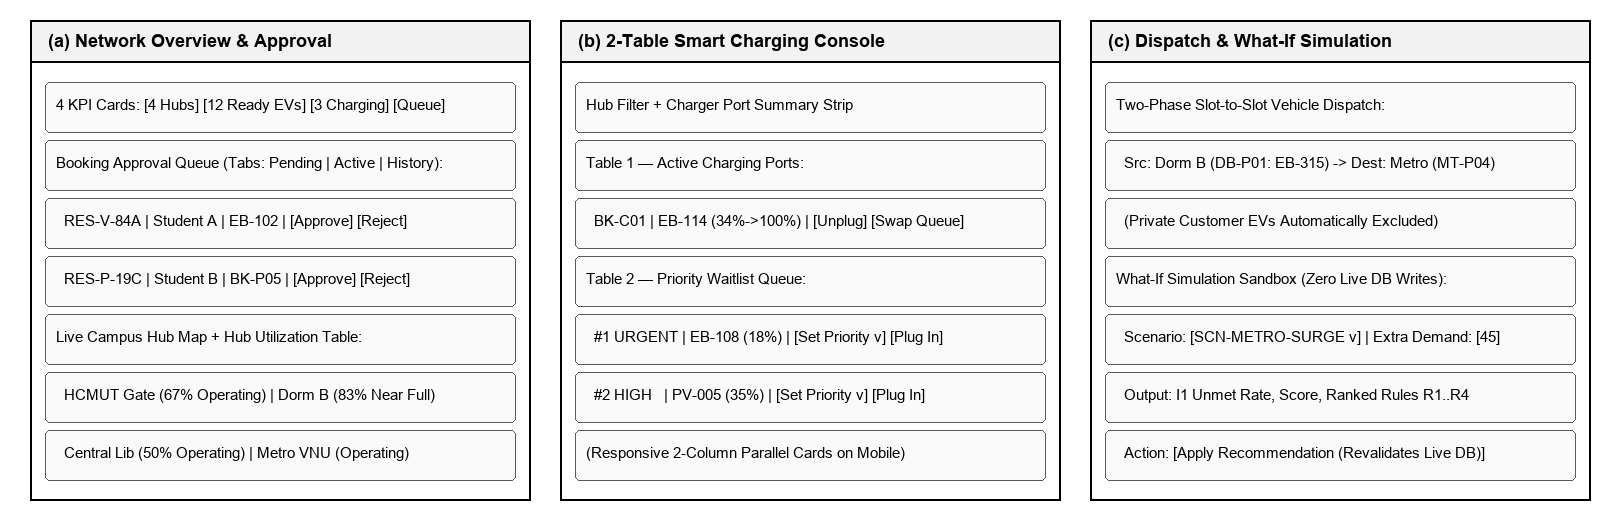
\includegraphics[width=0.94\linewidth]{graphics/diagrams/fig3_15_wf_operator.png}
  \caption{Operator Console V2.2 Structural Wireframes (Approval Queue, 2-Table Charging, What-If)}
  \label{fig:wf-operator}
\end{figure}

% --- UI PAGE PAIR A: Auth + 4-Hub Map ---
\begin{figure}[H]
  \centering
  \begin{subfigure}[t]{0.44\textwidth}
    \centering
    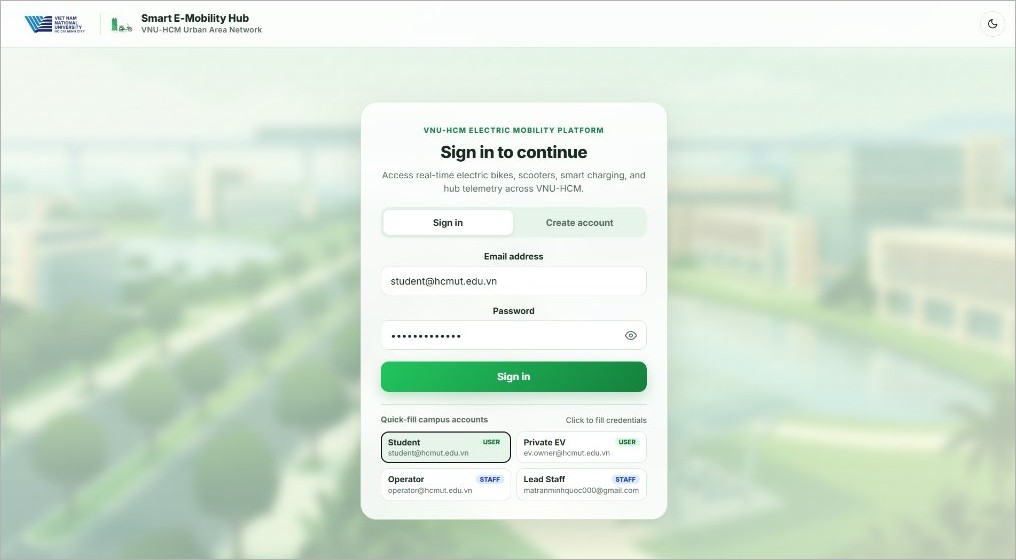
\includegraphics[width=\textwidth]{graphics/ui_v2/ui_login_student.jpg}
    \caption{Student Credential Autofill (\texttt{USER} Role)}
  \end{subfigure}\hspace{0.03\textwidth}%
  \begin{subfigure}[t]{0.44\textwidth}
    \centering
    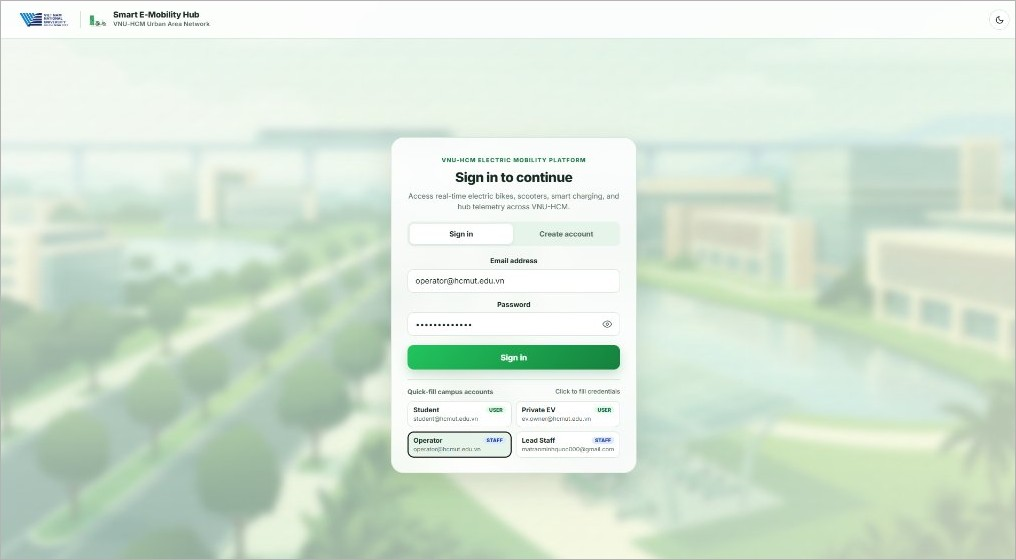
\includegraphics[width=\textwidth]{graphics/ui_v2/ui_login_operator.jpg}
    \caption{Hub Operator Credential Autofill (\texttt{OPERATOR} Role)}
  \end{subfigure}
  \caption{Delivered V2.2 Unified Authentication and Registration Interface}
  \label{fig:ui-auth}
\end{figure}

\begin{figure}[H]
  \centering
  \begin{subfigure}[t]{0.44\textwidth}
    \centering
    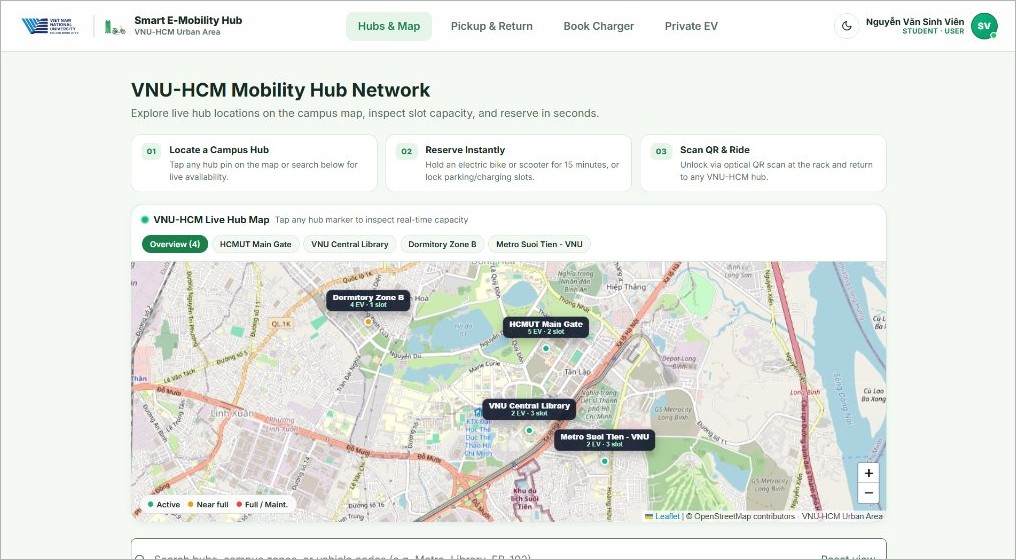
\includegraphics[width=\textwidth]{graphics/ui_v2/ui_hub_overview.jpg}
    \caption{VNU-HCM 4-Hub Network Overview \& 3-Step Guide}
  \end{subfigure}\hspace{0.03\textwidth}%
  \begin{subfigure}[t]{0.44\textwidth}
    \centering
    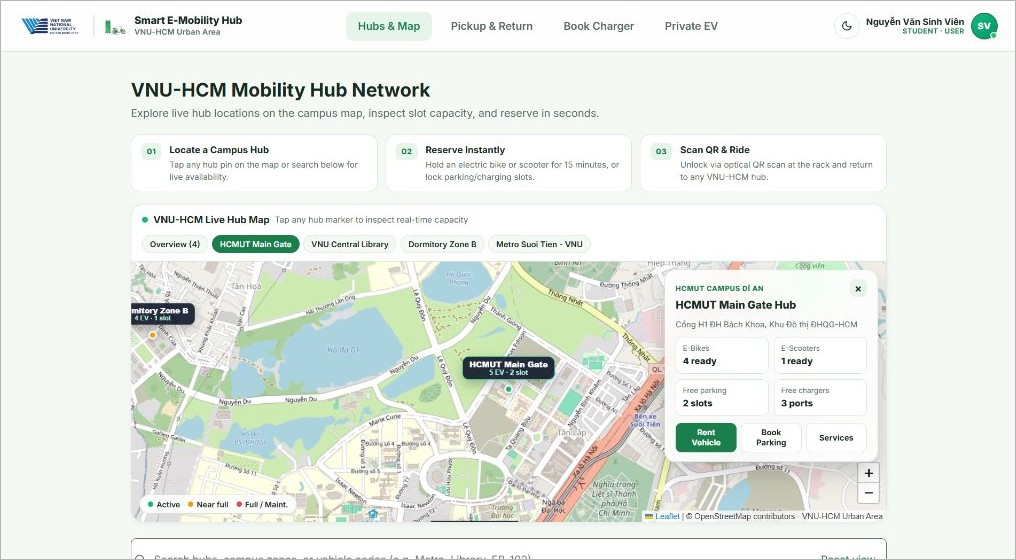
\includegraphics[width=\textwidth]{graphics/ui_v2/ui_hub_hcmut.jpg}
    \caption{HCMUT Main Gate Hub Live Capacity Card}
  \end{subfigure}\\[3pt]
  \begin{subfigure}[t]{0.44\textwidth}
    \centering
    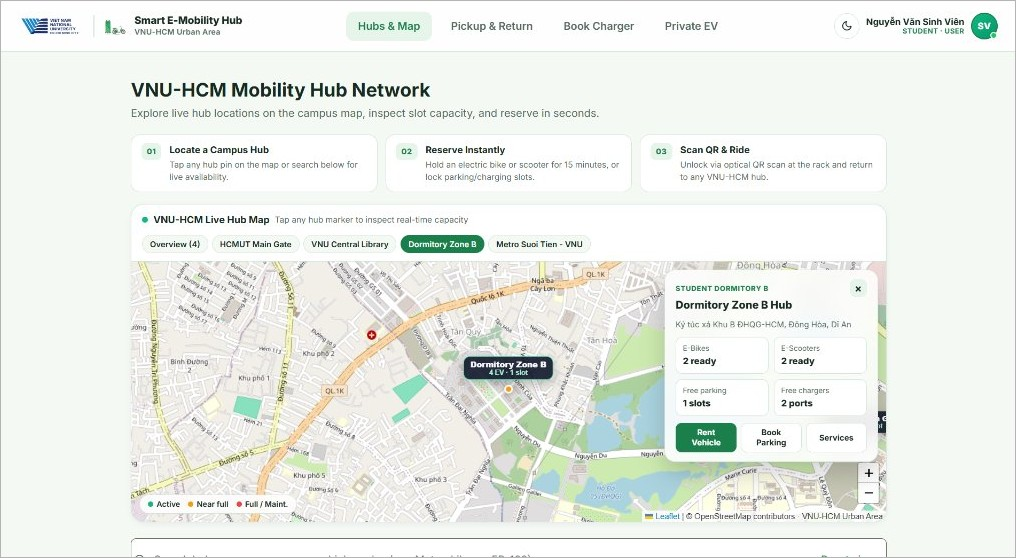
\includegraphics[width=\textwidth]{graphics/ui_v2/ui_hub_dormb.jpg}
    \caption{Dormitory Zone B Hub (\texttt{Near Full} Warning Pin)}
  \end{subfigure}\hspace{0.03\textwidth}%
  \begin{subfigure}[t]{0.44\textwidth}
    \centering
    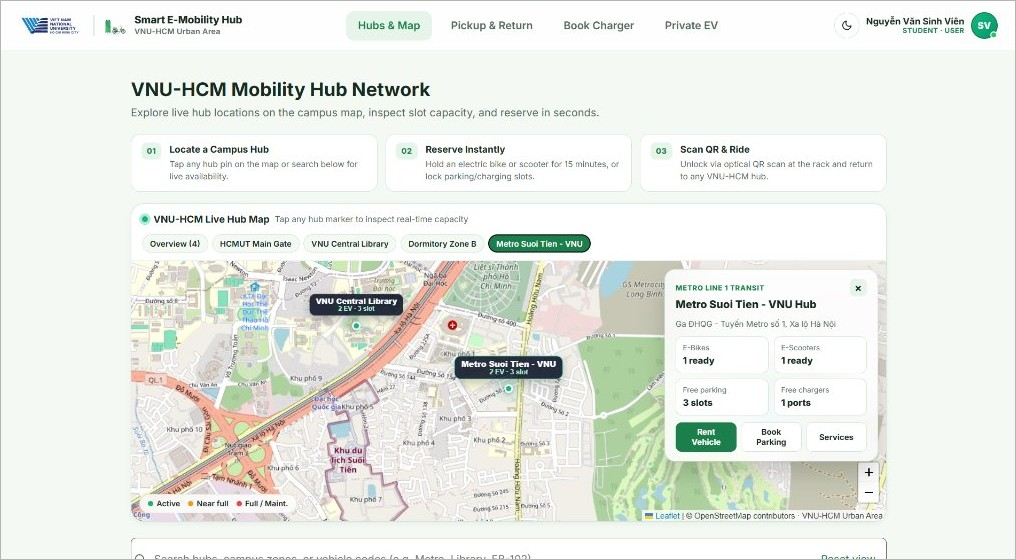
\includegraphics[width=\textwidth]{graphics/ui_v2/ui_hub_metro.jpg}
    \caption{Metro Suoi Tien -- VNU Line 1 Transit Hub}
  \end{subfigure}
  \caption{Delivered V2.2 Student Mobility Hub Network and Interactive OpenStreetMap Views (\texttt{UC01, UC02})}
  \label{fig:ui-student-map}
\end{figure}

% --- UI PAGE PAIR B: Student Flows + Operator Overview/Charging ---
\begin{figure}[H]
  \centering
  \begin{subfigure}[t]{0.44\textwidth}
    \centering
    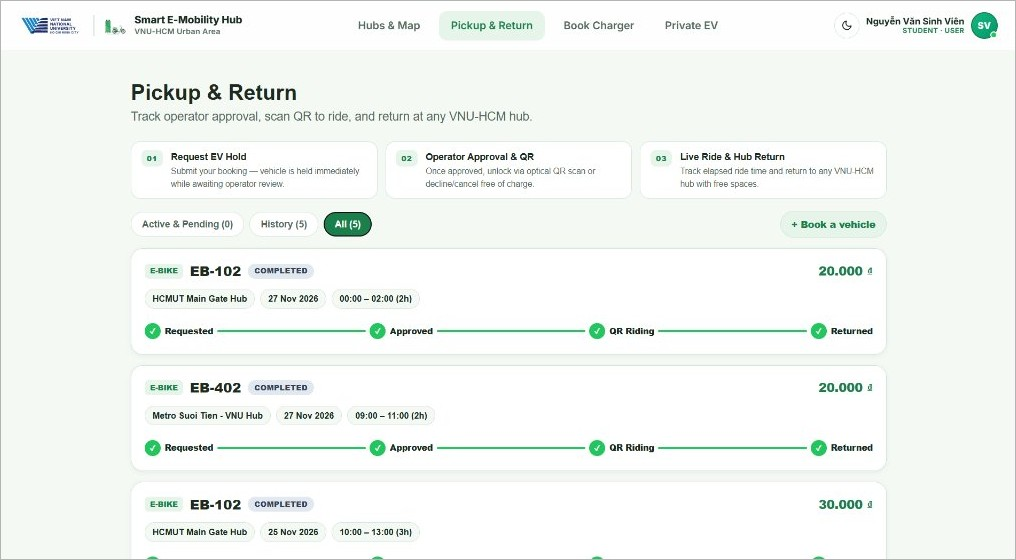
\includegraphics[width=\textwidth]{graphics/ui_v2/ui_res_completed.jpg}
    \caption{Completed Ride Stepper \& VND Tariff}
  \end{subfigure}\hspace{0.03\textwidth}%
  \begin{subfigure}[t]{0.44\textwidth}
    \centering
    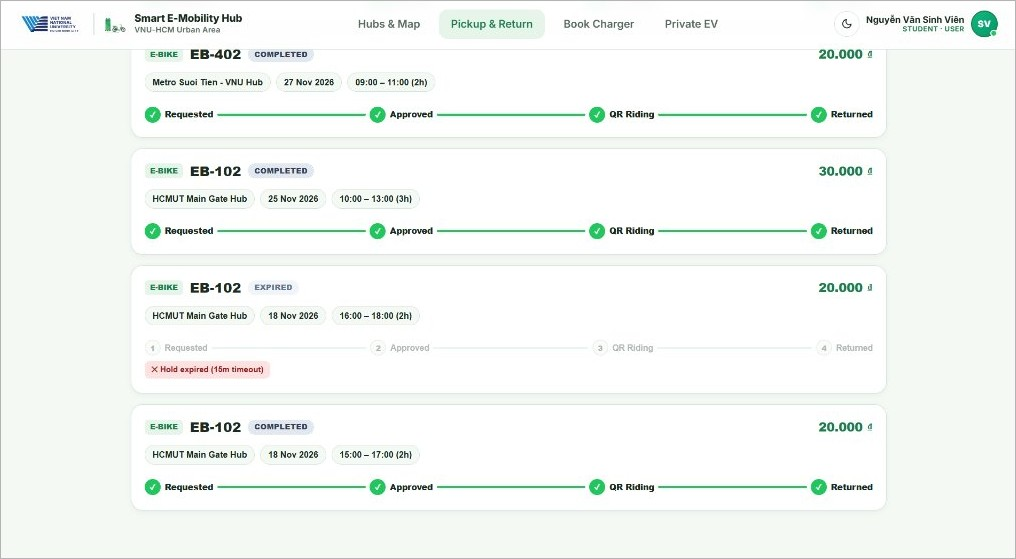
\includegraphics[width=\textwidth]{graphics/ui_v2/ui_res_expired.jpg}
    \caption{15-Minute Hold Expiration (\texttt{EXPIRED} Badge)}
  \end{subfigure}\\[3pt]
  \begin{subfigure}[t]{0.44\textwidth}
    \centering
    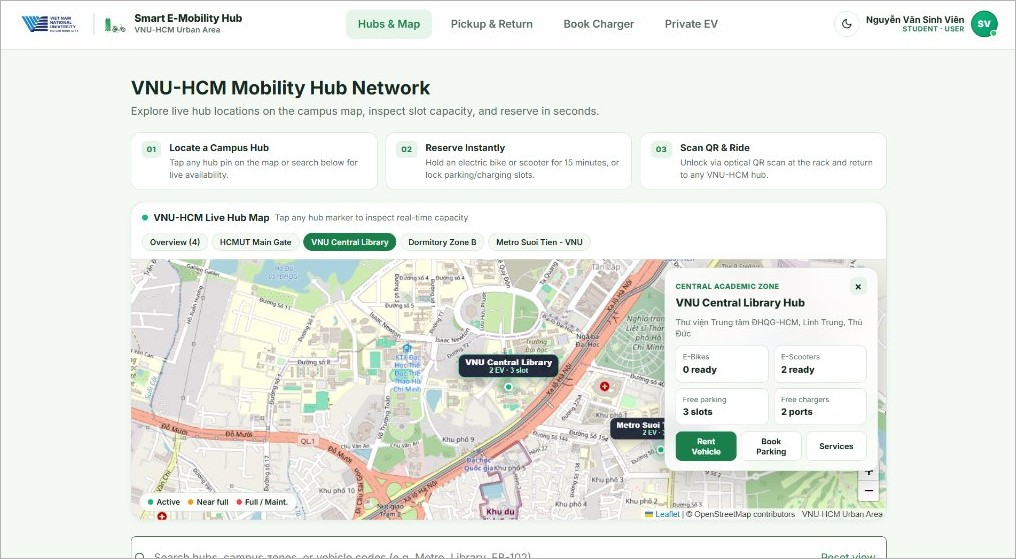
\includegraphics[width=\textwidth]{graphics/ui_v2/ui_hub_central.jpg}
    \caption{VNU Central Library Hub Selection View}
  \end{subfigure}\hspace{0.03\textwidth}%
  \begin{subfigure}[t]{0.44\textwidth}
    \centering
    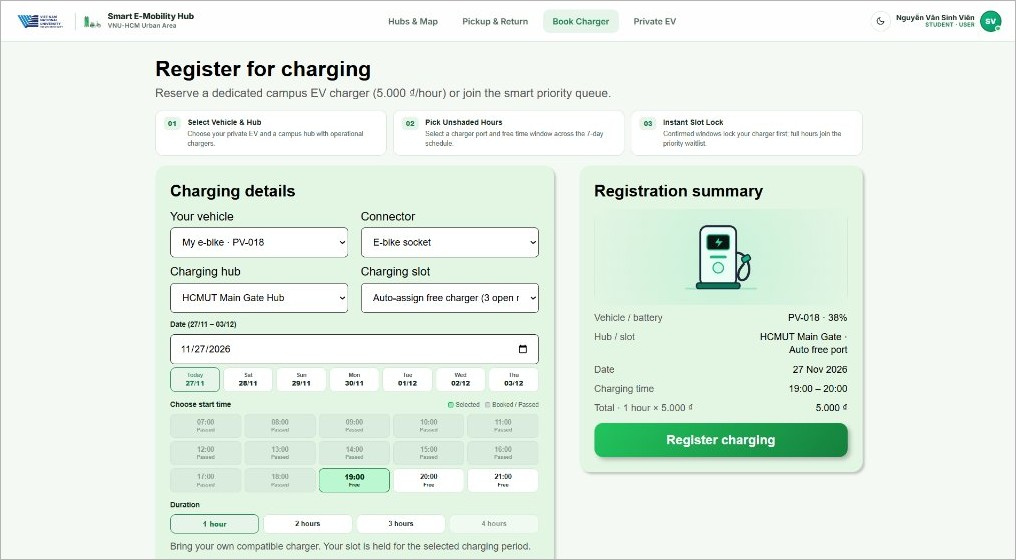
\includegraphics[width=\textwidth]{graphics/ui_v2/ui_charging_auto.jpg}
    \caption{7-Day Charger Booking with Default \texttt{AUTO} Mode}
  \end{subfigure}
  \caption{Delivered V2.2 Student Pickup/Return Lifecycle and Multi-Port \texttt{AUTO} Charger Registration (\texttt{UC04}--\texttt{UC09})}
  \label{fig:ui-student-flows}
\end{figure}

\begin{figure}[H]
  \centering
  \begin{subfigure}[t]{0.44\textwidth}
    \centering
    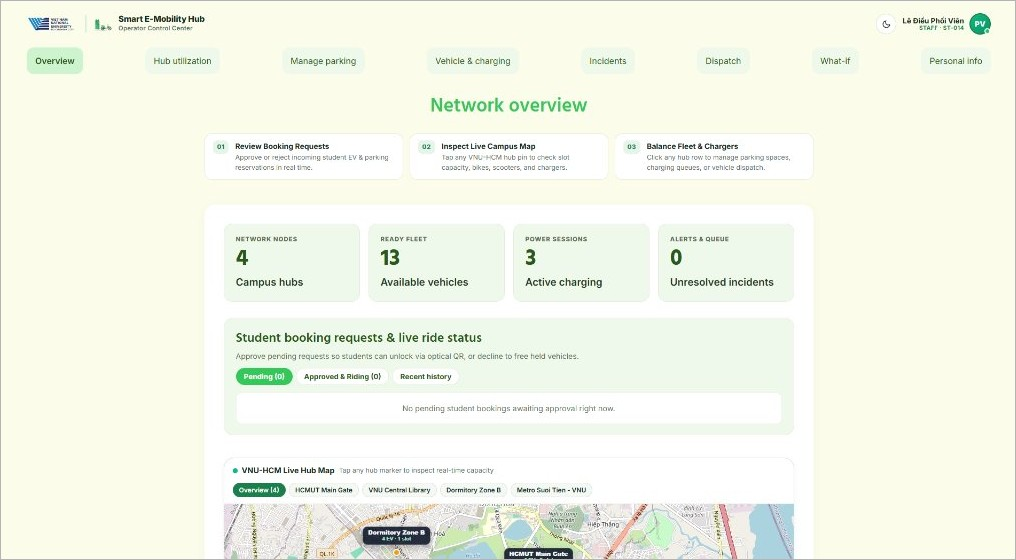
\includegraphics[width=\textwidth]{graphics/ui_v2/ui_op_overview.jpg}
    \caption{Operator Control Header \& 4 Prominent KPI Cards}
  \end{subfigure}\hspace{0.03\textwidth}%
  \begin{subfigure}[t]{0.44\textwidth}
    \centering
    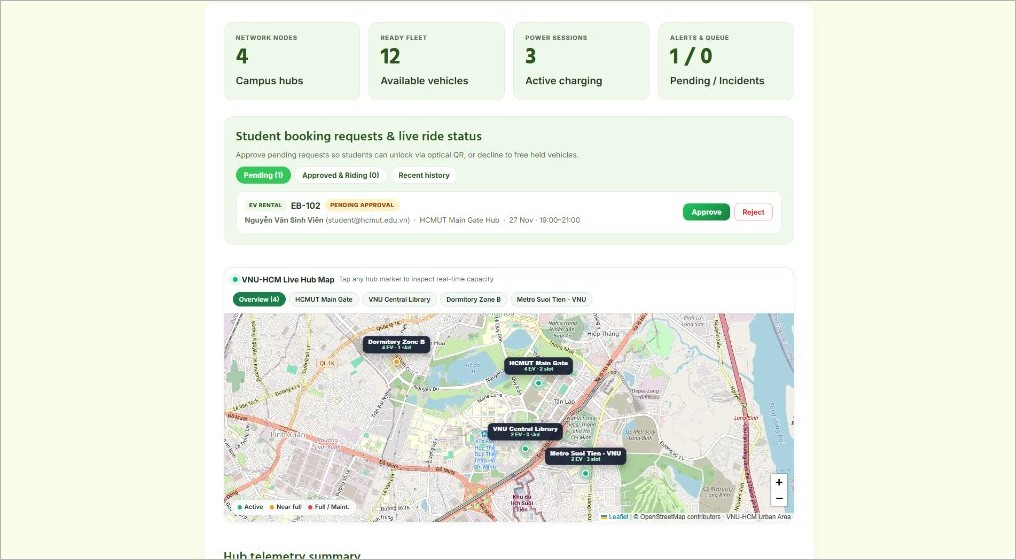
\includegraphics[width=\textwidth]{graphics/ui_v2/ui_op_approval.jpg}
    \caption{Live Booking Approval Queue (\texttt{Approve} / \texttt{Reject})}
  \end{subfigure}\\[3pt]
  \begin{subfigure}[t]{0.44\textwidth}
    \centering
    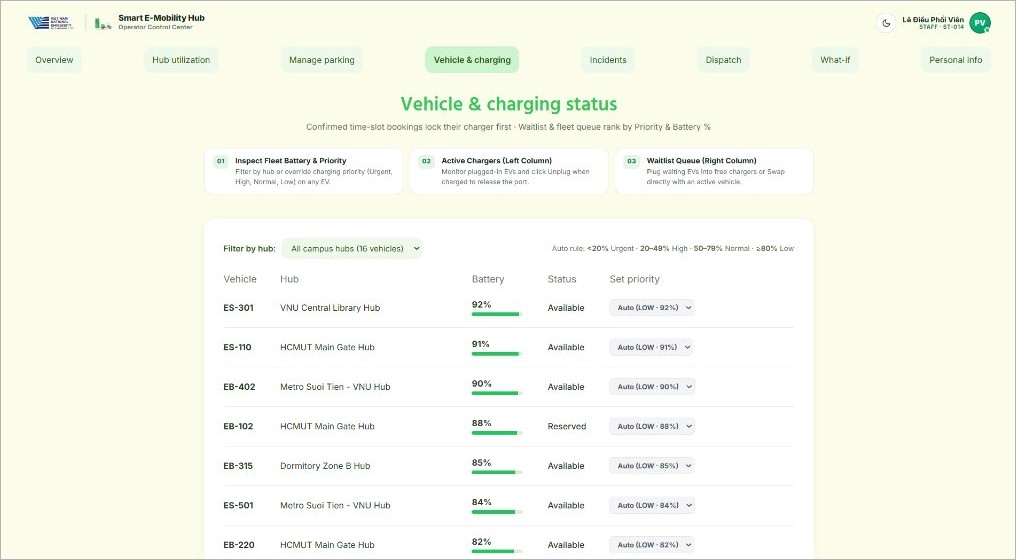
\includegraphics[width=\textwidth]{graphics/ui_v2/ui_op_fleet_soc.jpg}
    \caption{Fleet Battery Telemetry \& Priority Rules}
  \end{subfigure}\hspace{0.03\textwidth}%
  \begin{subfigure}[t]{0.44\textwidth}
    \centering
    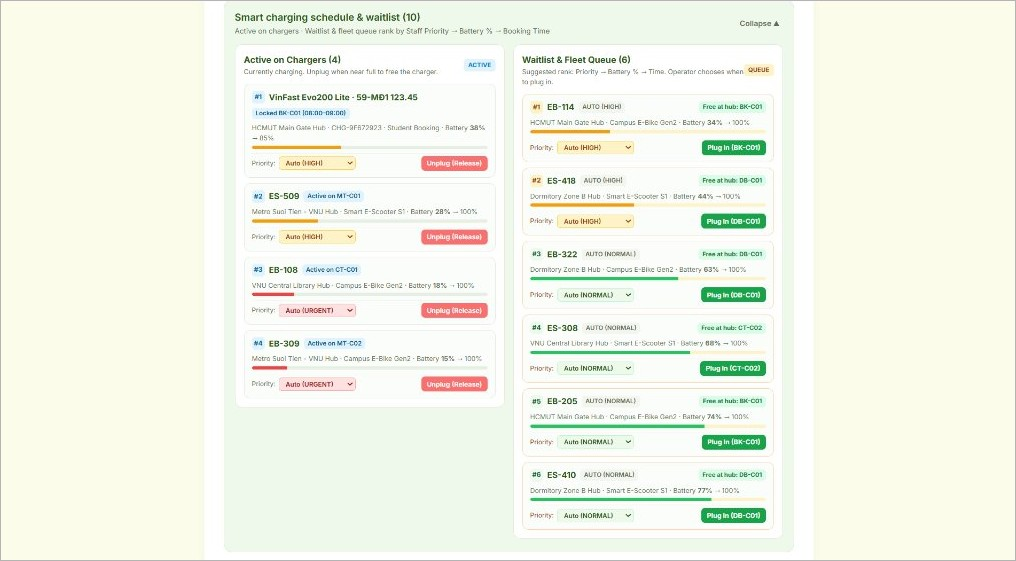
\includegraphics[width=\textwidth]{graphics/ui_v2/ui_op_charging_split.jpg}
    \caption{2-Table Split: Active Chargers vs.\ Priority Queue}
  \end{subfigure}
  \caption{Delivered V2.2 Operator Network Overview, Booking Approval, and Smart Charging Console (\texttt{UC04, UC10, UC15})}
  \label{fig:ui-operator-console}
\end{figure}

% --- UI PAGE PAIR C: Operator Ops + Mobile Dark-Mode LAN ---
\begin{figure}[H]
  \centering
  \begin{subfigure}[t]{0.44\textwidth}
    \centering
    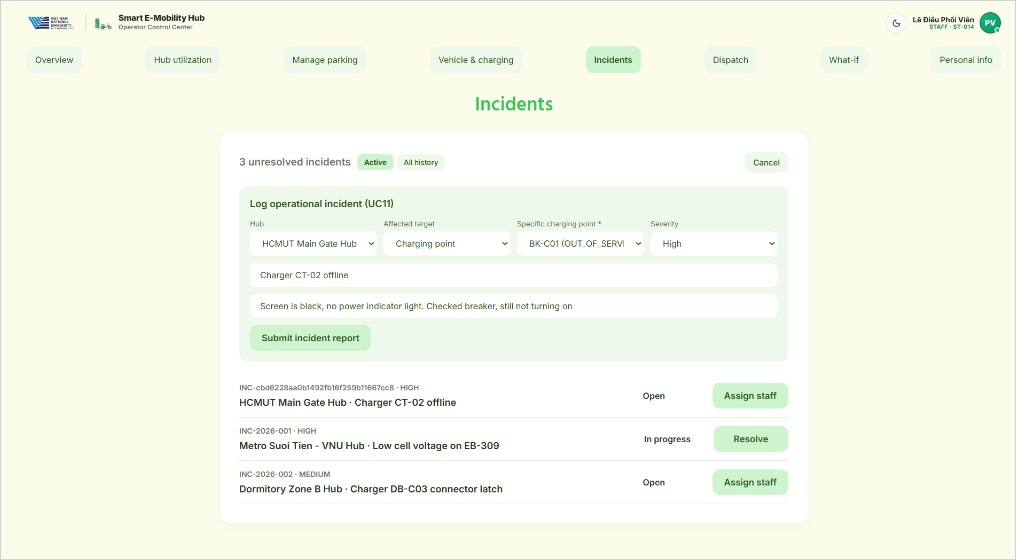
\includegraphics[width=\textwidth]{graphics/ui_v2/ui_op_incidents.jpg}
    \caption{Mandatory-Target Incident Isolation (\texttt{UC11, UC12})}
  \end{subfigure}\hspace{0.03\textwidth}%
  \begin{subfigure}[t]{0.44\textwidth}
    \centering
    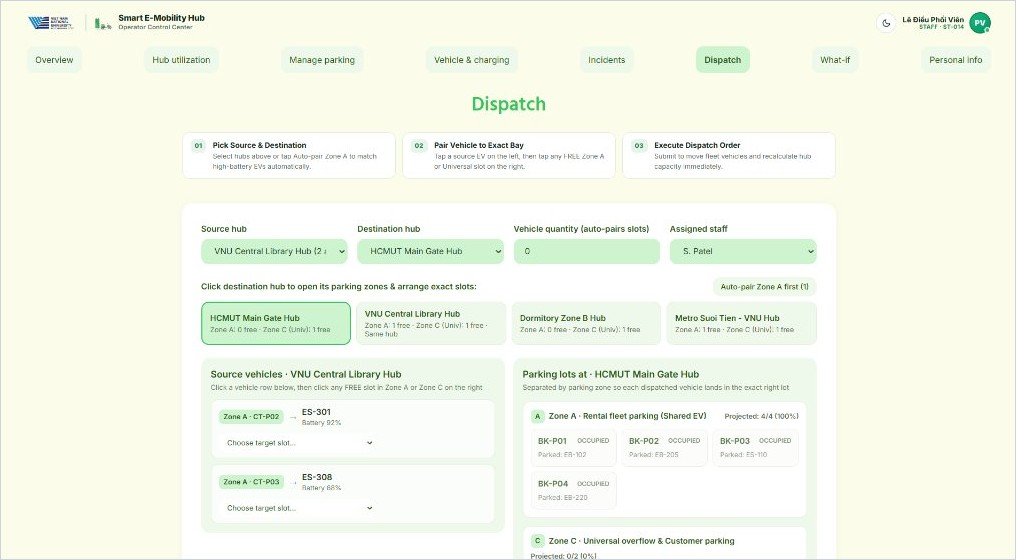
\includegraphics[width=\textwidth]{graphics/ui_v2/ui_op_dispatch.jpg}
    \caption{Slot-to-Slot Dispatch Across Zones A \& C (\texttt{UC13})}
  \end{subfigure}\\[3pt]
  \begin{subfigure}[t]{0.44\textwidth}
    \centering
    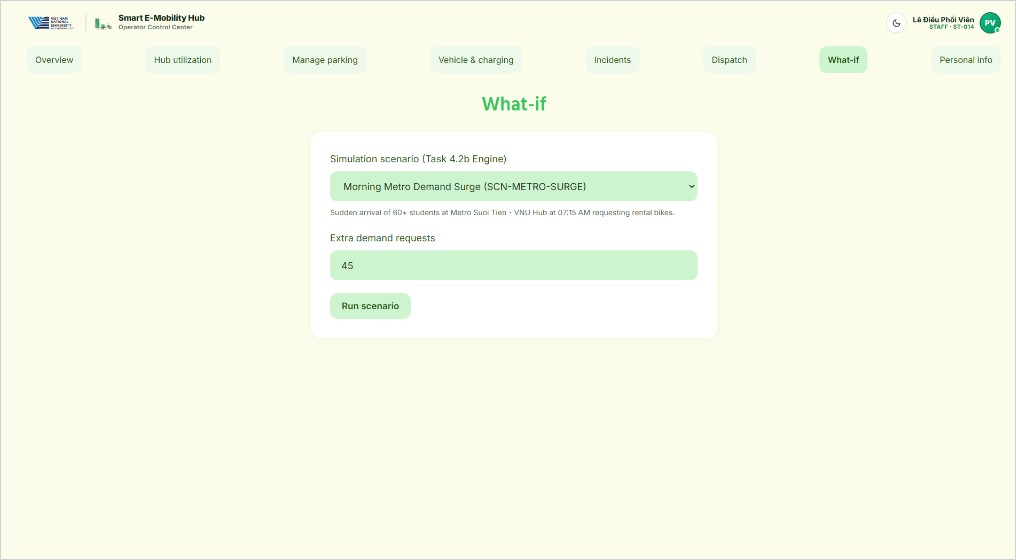
\includegraphics[width=\textwidth]{graphics/ui_v2/ui_op_whatif.jpg}
    \caption{Isolated What-If Engine (\texttt{SCN-METRO-SURGE}, \texttt{UC16})}
  \end{subfigure}\hspace{0.03\textwidth}%
  \begin{subfigure}[t]{0.44\textwidth}
    \centering
    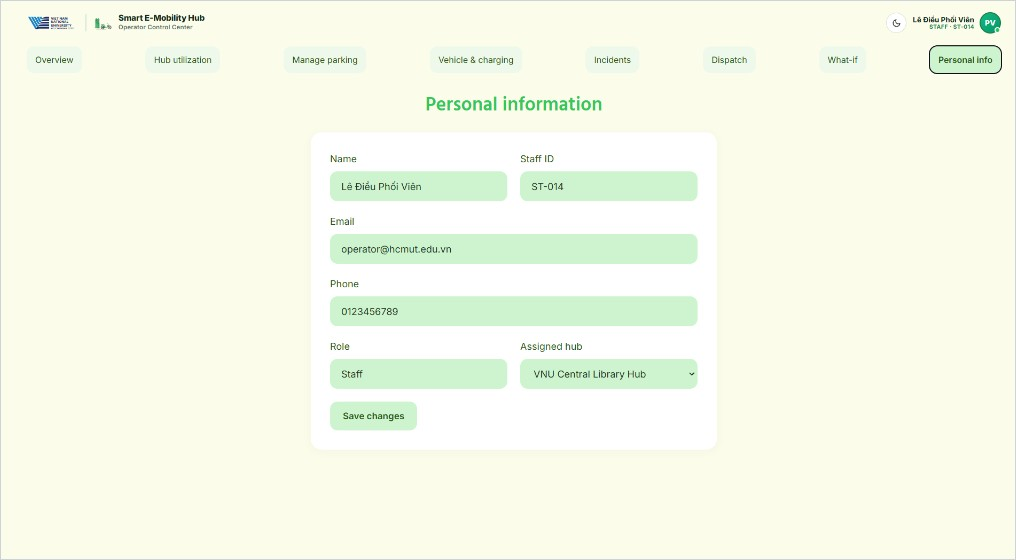
\includegraphics[width=\textwidth]{graphics/ui_v2/ui_op_profile.jpg}
    \caption{Operator Staff Profile \& Assigned Hub (\texttt{ST-014})}
  \end{subfigure}
  \caption{Delivered V2.2 Operator Incident Isolation, Slot-to-Slot Dispatch, What-If Simulation, and Staff Profile Views (\texttt{UC11}--\texttt{UC18})}
  \label{fig:ui-operator-ops}
\end{figure}

\begin{figure}[H]
  \centering
  \begin{subfigure}[t]{0.26\textwidth}
    \centering
    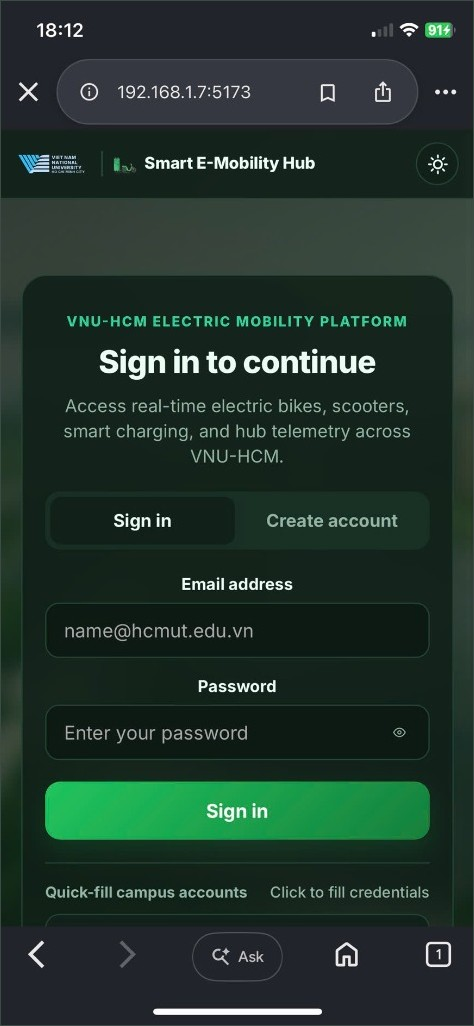
\includegraphics[width=\textwidth]{graphics/ui_v2/ui_mob_lan_url.jpg}
    \caption{Wi-Fi LAN (\texttt{192.168.1.7:5173})}
  \end{subfigure}\hspace{0.03\textwidth}%
  \begin{subfigure}[t]{0.26\textwidth}
    \centering
    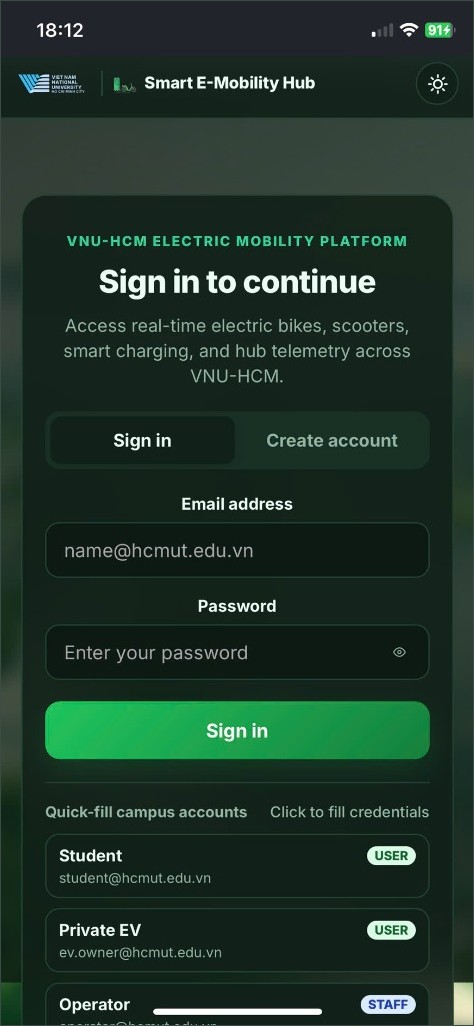
\includegraphics[width=\textwidth]{graphics/ui_v2/ui_mob_login_dark.jpg}
    \caption{Dark-Mode Auth \& Demo Chips}
  \end{subfigure}\hspace{0.03\textwidth}%
  \begin{subfigure}[t]{0.26\textwidth}
    \centering
    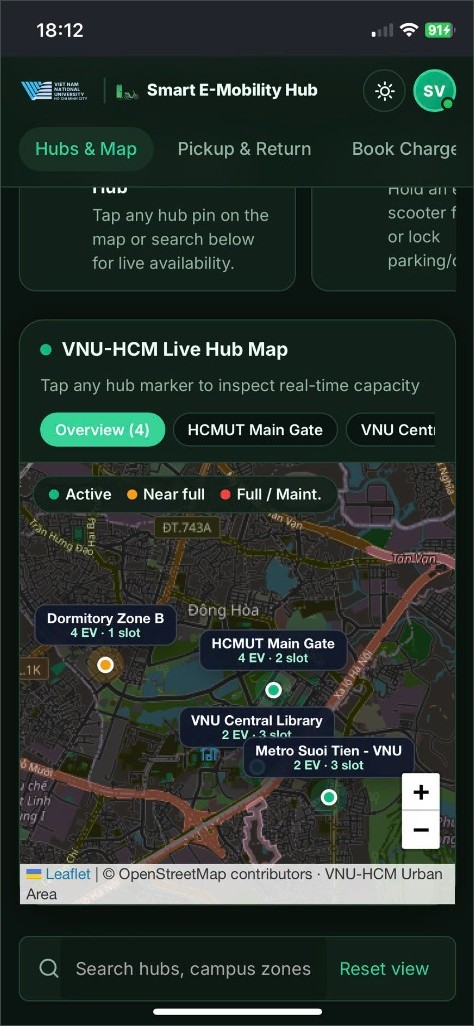
\includegraphics[width=\textwidth]{graphics/ui_v2/ui_mob_map_dark.jpg}
    \caption{Responsive Dark Live Hub Map}
  \end{subfigure}
  \caption{Delivered V2.2 Responsive Mobile Interfaces in Dark Mode over Campus Wi-Fi LAN (\texttt{192.168.1.7:5173})}
  \label{fig:ui-mobile-lan}
\end{figure}

\begin{table}[H]
  \centering
  \singlespacing\footnotesize
  \caption{Summary of Student Portal and Operator Console Screens and Feedback Mechanisms}
  \label{tab:ui-screens}
  \renewcommand{\arraystretch}{1.22}
  \begin{tabularx}{\textwidth}{|L{3.9cm}|C{1.5cm}|L{4.1cm}|Y|}
    \hline
    \rowcolor{tblHeader}
    \textbf{Screen / Route} & \textbf{Actor} & \textbf{Information Presented} & \textbf{User Actions, Feedback \& Usability Rationale} \\
    \hline
    Login \& Registration\newline(\texttt{/login}) & \texttt{A1, A2} & Email/password form, sign-up tab, VNU-HCM demo chips. & One-click demo credential autofill, password validation, automatic role routing. \\
    \hline
    Hubs \& Live Map\newline(\texttt{/student/hubs}) & \texttt{A1} & 2D OpenStreetMap pins, 3-step onboarding strip, live bike/scooter/slot counts. & Tap map pins, filter by EV type, search autocomplete; color-coded saturation badges. \\
    \hline
    Pickup \& Return\newline(\texttt{/student/\allowbreak reservations}) & \texttt{A1} & 5-stage progress stepper, EV SoC, rack code, VND fee, elapsed ride timer. & Submit hold, $4\text{ s}$ live approval sync, optical QR unlock, role-safe cancel, return hub selector. \\
    \hline
    Book Parking \& Charger\newline(\texttt{/student/\allowbreak charging}) & \texttt{A1} & 7-day hour grid, \texttt{AUTO} port/bay selector, $100\%$ target SoC, VND summary. & Hours remain selectable until \emph{all} hub ports/bays are booked, preventing false port collisions. \\
    \hline
    Network Overview\newline(\texttt{/operator/\allowbreak dashboard}) & \texttt{A2} & 4 prominent KPI cards, Booking Approval Queue, live map, utilization table. & Instant \textit{Approve} / \textit{Reject} buttons with toast confirmation and 10-second telemetry refresh. \\
    \hline
    2-Table Charging \& Parking\newline(\texttt{/operator/*}) & \texttt{A2} & Parallel Active Chargers vs.\ Priority Waitlist tables; Zones A/B/C slot cards. & \texttt{Set Priority} (\texttt{URGENT..LOW}), \texttt{Plug-in}, \texttt{Swap}, \texttt{Unplug}, and Zone C check-in/out; 2-column mobile grid. \\
    \hline
    Incidents, Dispatch \& What-If\newline(\texttt{/operator/*}) & \texttt{A2} & Open/closed incidents, slot-to-slot builder, scenario controls \& \texttt{I1..I8} metrics. & Mandatory target-unit picker, private-EV exclusion in dispatch, isolated Before/After simulation preview. \\
    \hline
    Mobile Dark-Mode LAN\newline(\texttt{192.168.1.7:\allowbreak 5173}) & \texttt{A1, A2} & Portrait single-column cards, dark-themed Leaflet tiles, touch pill navigation. & Zero horizontal overflow across $360\text{ px}$--$430\text{ px}$ viewports, Dark/Light toggle, live LAN API sync. \\
    \hline
  \end{tabularx}
\end{table}

\clearpage
\section{Software Architecture, Data Model, and What-If Simulation Design}
\label{sec:architecture-data-sim}

\safesubsection{Software Architecture}
\label{subsec:software-architecture}
The Smart E-Mobility Hub is architected as a \textbf{Three-Tier Layered Modular Monolith} (\Cref{fig:architecture}), complemented by a formal UML 2.5 Component Diagram (\Cref{fig:component}) and a Campus Wi-Fi/LAN Deployment Topology (\Cref{fig:deployment}).

\begin{figure}[H]
  \centering
  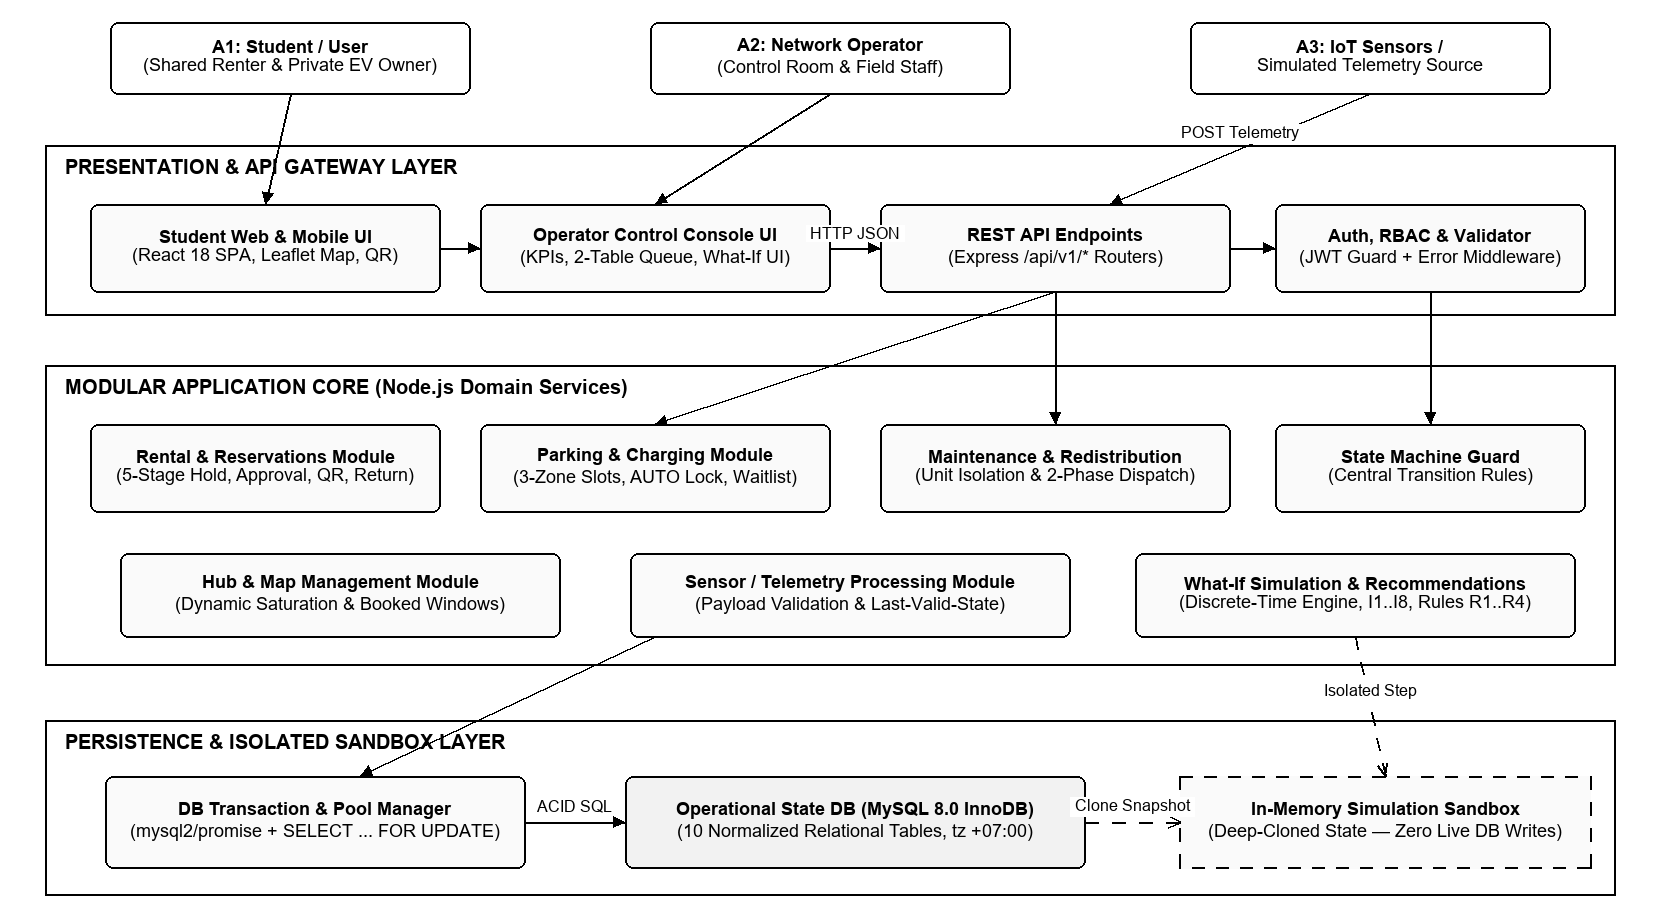
\includegraphics[width=0.95\linewidth]{graphics/diagrams/fig4_1_architecture.png}
  \caption{High-Level Three-Tier Modular Monolithic Software Architecture}
  \label{fig:architecture}
\end{figure}

\begin{itemize}
  \item \textbf{Component Responsibilities:} (1) The \emph{Presentation \& API Gateway Layer} hosts the React 18 Student/Operator SPAs, Express \texttt{/api/v1} REST routers, JWT/RBAC guards, and input/error middlewares; (2) the \emph{Modular Application Core} houses seven cohesive domain modules (\texttt{Rental \& Reservations}, \texttt{Parking \& Charging}, \texttt{Maintenance \& Redistribution}, \texttt{Hub \& Map Management}, \texttt{Telemetry Processing}, \texttt{What-If Simulation}, and the central \texttt{State Machine Guard}); and (3) the \emph{Persistence \& Sandbox Layer} separates transactional MySQL 8.0 InnoDB storage from the ephemeral In-Memory Simulation Sandbox.
  \item \textbf{Communication, Business Logic Location \& Isolation:} External clients communicate via stateless HTTP/JSON REST requests; internal core modules invoke one another synchronously in-process while sharing an InnoDB transaction connection (\texttt{withTransaction}) to enforce multi-table ACID atomicity. \emph{All domain business rules reside strictly inside Application Core services.} What-If runs read a consistent MySQL snapshot and evolve a deep-cloned object graph in RAM (\texttt{0} live DB writes).
\end{itemize}

\begin{figure}[H]
  \centering
  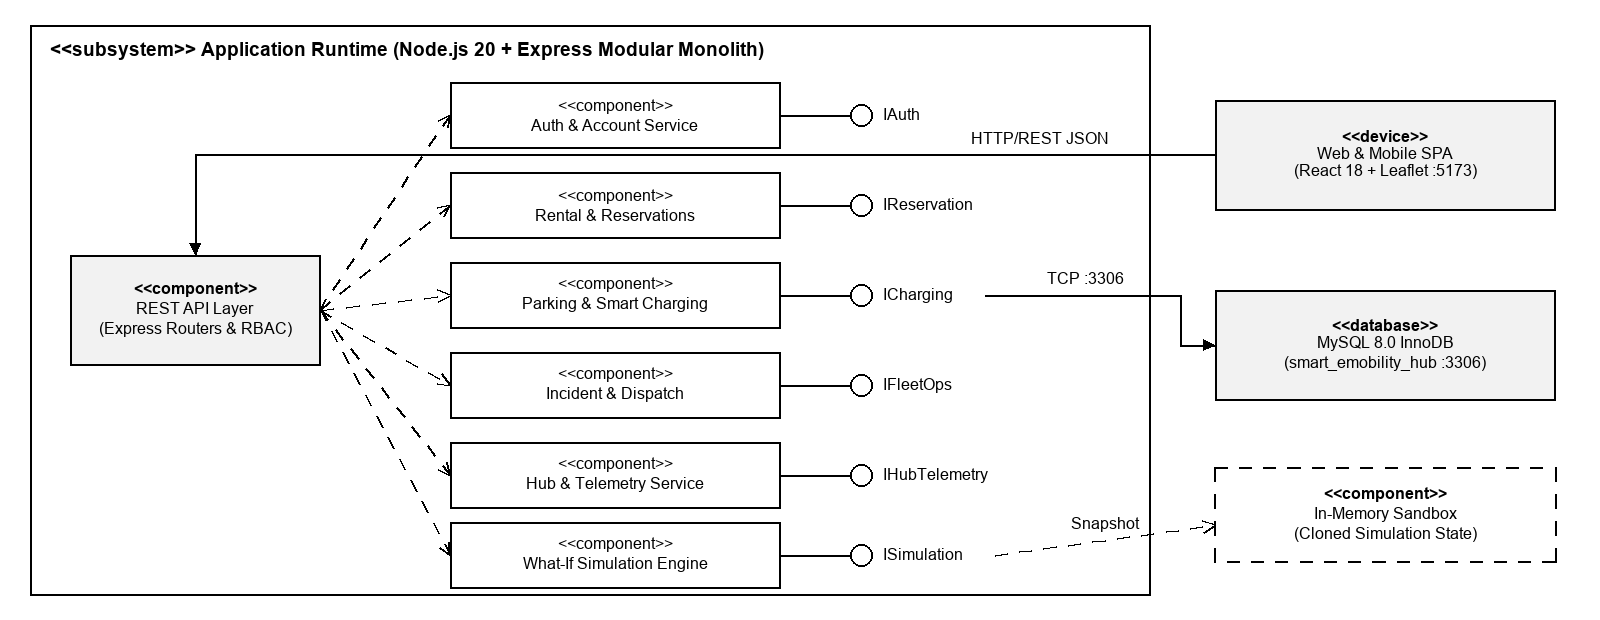
\includegraphics[width=0.92\linewidth]{graphics/diagrams/fig4_2_component.png}
  \caption{UML 2.5 Component Diagram with Provided and Required Interfaces}
  \label{fig:component}
\end{figure}

\begin{figure}[H]
  \centering
  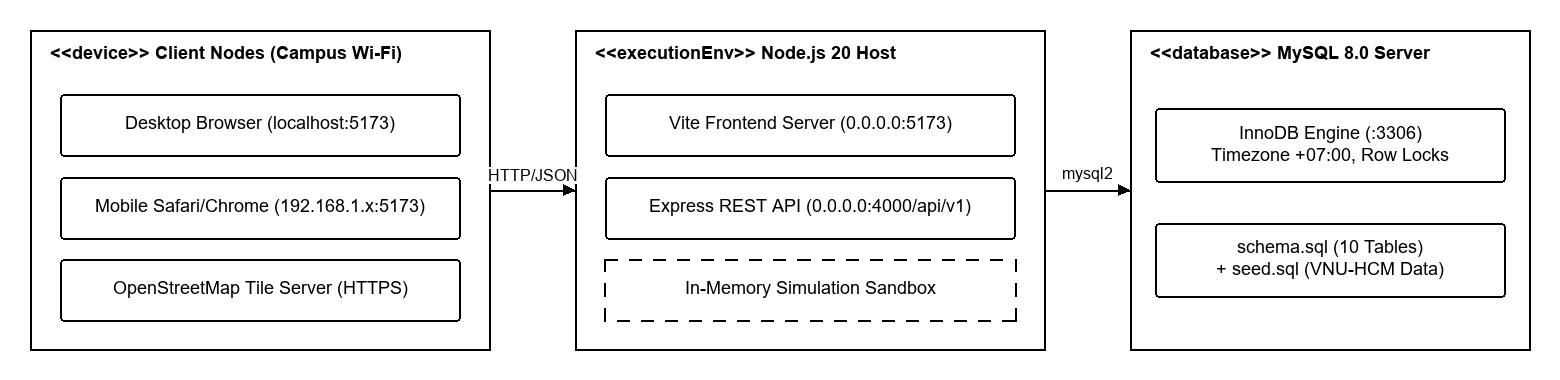
\includegraphics[width=0.92\linewidth]{graphics/diagrams/fig4_3_deployment.png}
  \caption{Campus Wi-Fi / LAN Runtime Deployment Topology}
  \label{fig:deployment}
\end{figure}

\begin{table}[H]
  \centering
  \singlespacing\footnotesize
  \caption{Architectural Comparison and Trade-Off Justification}
  \label{tab:arch-tradeoffs}
  \renewcommand{\arraystretch}{1.23}
  \begin{tabularx}{\textwidth}{|L{3.3cm}|L{4.3cm}|Y|}
    \hline
    \rowcolor{tblHeader}
    \textbf{Architecture Style} & \textbf{Benefits for Project Scope} & \textbf{Trade-Offs \& Selection Decision} \\
    \hline
    \textbf{Three-Tier Modular Monolith + MySQL 8.0 (Selected)} & Single-node InnoDB \texttt{FOR UPDATE} row locks prevent cross-table double-booking; zero inter-service RPC latency; simple campus LAN hosting. & Single-database vertical scaling ceiling and shared Node.js RAM for simulations (mitigated by $30\text{ s}$ cap). \textbf{Selected.} \\
    \hline
    \textbf{Distributed Microservices} & Independent horizontal scaling per domain service. & Requires distributed sagas across Vehicle, Slot, and Hub state updates, creating eventual-consistency race windows. \textbf{Rejected.} \\
    \hline
    \textbf{Document Store (MongoDB)} & Schema-less JSON storage for telemetry logs. & Weaker relational foreign-key guarantees across 10 normalized resource tables. \textbf{Rejected in favor of MySQL 8.0.} \\
    \hline
  \end{tabularx}
\end{table}

\safesubsection{Structural Class Diagram and Physical MySQL 8.0 ERD}
\label{subsec:structural-data}
\Cref{fig:class-diagram} models the implementation-oriented UML Class Diagram (\texttt{<<entity>>}, \texttt{<<service>>}, attributes, operations, and multiplicities), while \Cref{fig:erd} and \Cref{tab:db-tables} specify the 10 normalized MySQL 8.0 InnoDB tables defined in the physical relational schema. Conceptual Phase 2B entities (19 draft classes separating vehicle/parking reservations and simulation logs) were consolidated into 10 normalized tables (\texttt{reservations} unified via \texttt{reservation\_\allowbreak type}; simulation runs held in RAM) to eliminate multi-table join anomalies and enforce strict operational state isolation.

\begin{figure}[H]
  \centering
  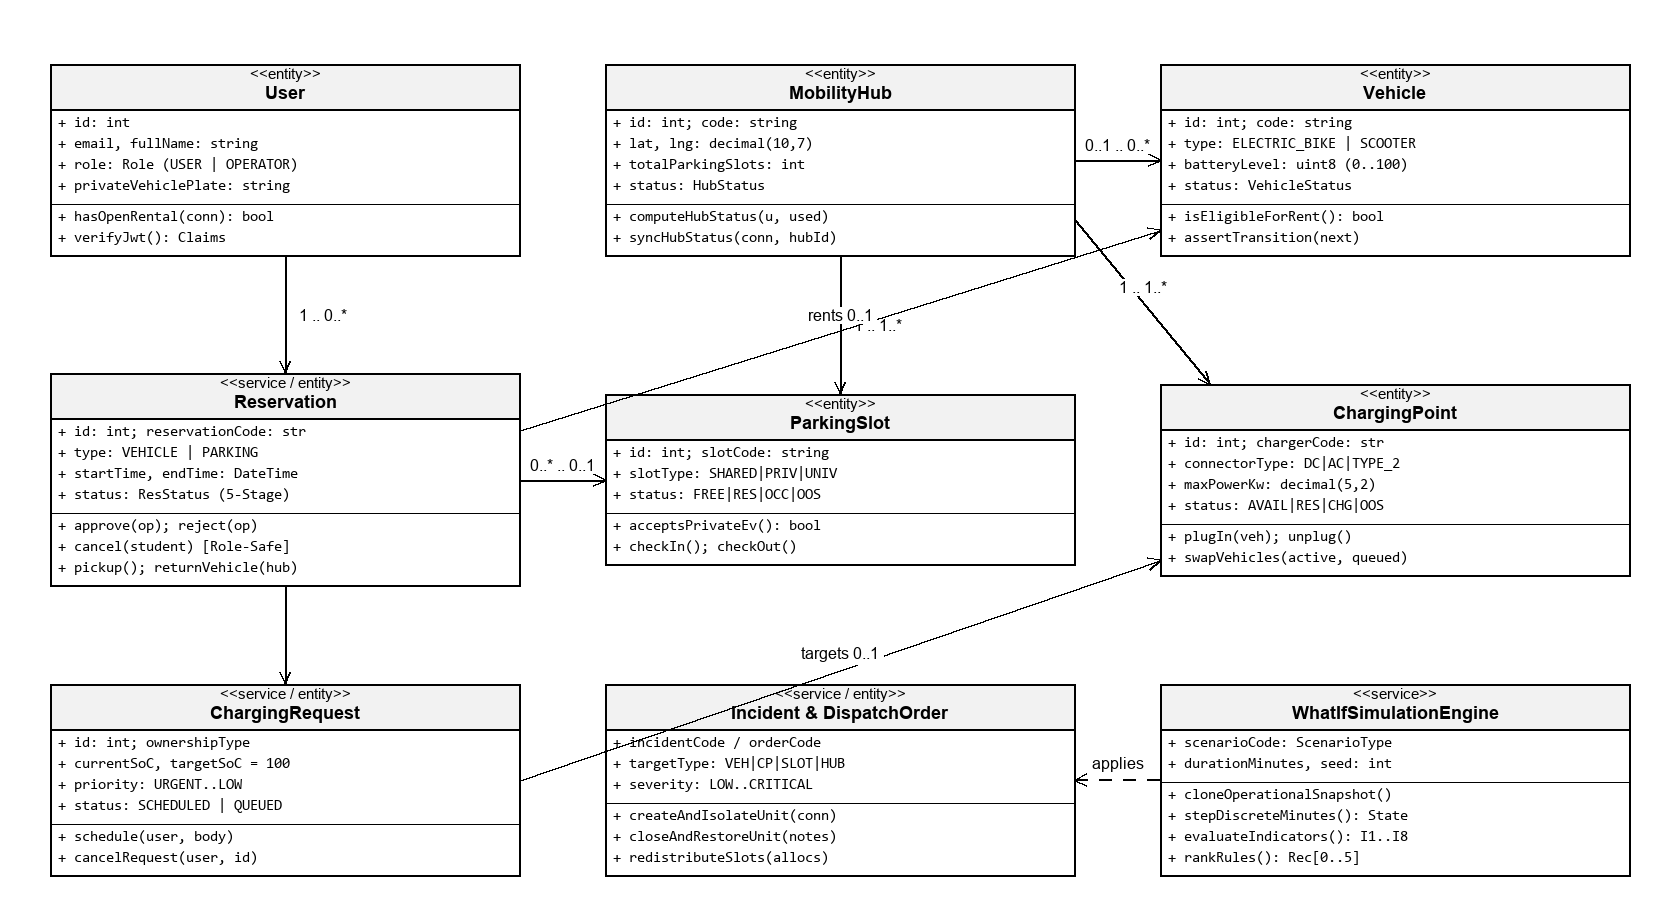
\includegraphics[width=0.92\linewidth]{graphics/diagrams/fig4_4_class_diagram.png}
  \caption{Implementation-Oriented UML Class Diagram}
  \label{fig:class-diagram}
\end{figure}

\begin{figure}[H]
  \centering
  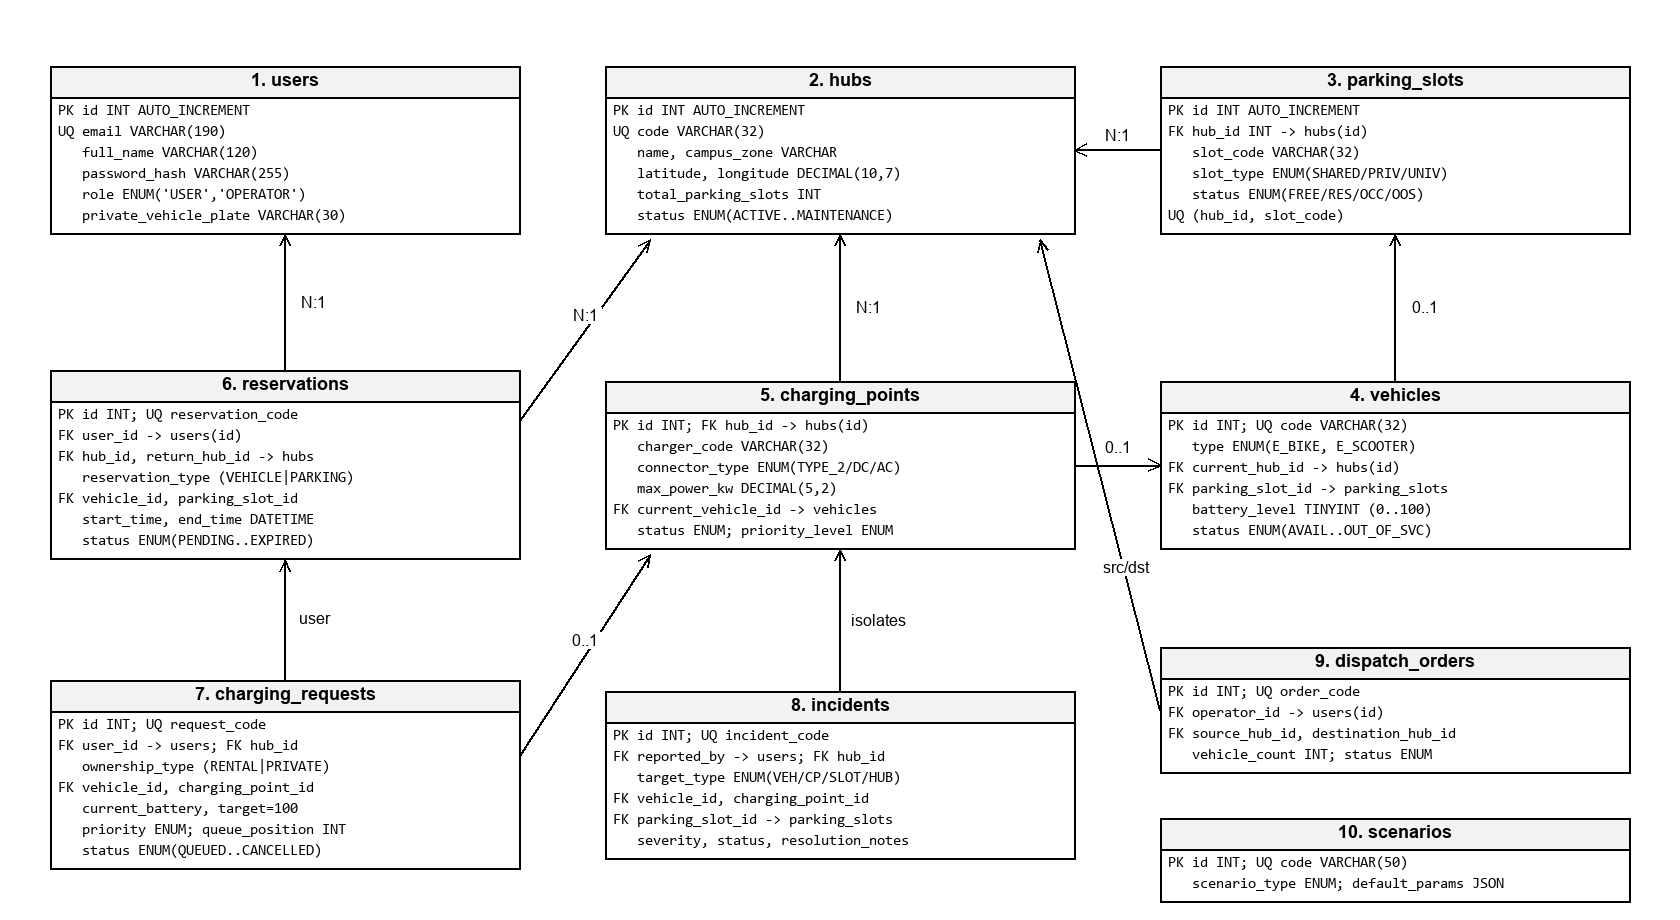
\includegraphics[width=0.92\linewidth]{graphics/diagrams/fig4_5_erd.png}
  \caption{Physical MySQL 8.0 Entity-Relationship Diagram (10 Normalized InnoDB Tables)}
  \label{fig:erd}
\end{figure}

\begin{table}[H]
  \centering
  \singlespacing\footnotesize
  \caption{Physical MySQL 8.0 Relational Tables, Keys, and Domain Roles}
  \label{tab:db-tables}
  \renewcommand{\arraystretch}{1.22}
  \begin{tabularx}{\textwidth}{|L{3.5cm}|L{4.3cm}|Y|}
    \hline
    \rowcolor{tblHeader}
    \textbf{Table Name} & \textbf{Primary \& Key Foreign Keys} & \textbf{Stored Operational State \& Constraints} \\
    \hline
    \texttt{users} & \texttt{PK id}; \texttt{UQ email} & User credentials, RBAC role (\texttt{USER} $|$ \texttt{OPERATOR}), per-user mutex target. \\
    \hline
    \texttt{hubs} & \texttt{PK id}; \texttt{UQ code} & GPS coordinates, capacities, dynamic saturation (\texttt{ACTIVE..MAINTENANCE}). \\
    \hline
    \texttt{parking\_slots} & \texttt{PK id}; \texttt{FK hub\_id};\newline\texttt{UQ(hub, code)} & Zone type (\texttt{SHARED\_\allowbreak EV} $|$ \texttt{PRIVATE\_\allowbreak EV} $|$ \texttt{UNIVERSAL}) and slot state. \\
    \hline
    \texttt{vehicles} & \texttt{PK id}; \texttt{FK current\_\allowbreak hub\_id}, \texttt{slot\_id} & Shared bikes/scooters, $\text{SoC} \in [0,100]$, range, lifecycle status. \\
    \hline
    \texttt{charging\_points} & \texttt{PK id}; \texttt{FK hub\_id},\newline\texttt{current\_\allowbreak vehicle\_id} & Connector type, kW rating, port state (\texttt{AVAILABLE..OUT\_\allowbreak OF\_\allowbreak SERVICE}). \\
    \hline
    \texttt{reservations} & \texttt{PK id}; \texttt{FK user\_id}, \texttt{hub\_id}, \texttt{vehicle\_id}, \texttt{slot\_id} & Unified 5-stage rental \& parking bookings (\texttt{PENDING..COMPLETED/\allowbreak EXPIRED}). \\
    \hline
    \texttt{charging\_requests} & \texttt{PK id}; \texttt{FK user\_id}, \texttt{hub\_id},\newline\texttt{charging\_\allowbreak point\_id} & Scheduled port locks (\texttt{SCHEDULED}) and priority waitlist (\texttt{QUEUED}, $100\%$). \\
    \hline
    \texttt{incidents} & \texttt{PK id}; \texttt{FK reported\_by}, \texttt{hub\_id}, \texttt{unit\_ids} & Mandatory target unit fault logs, severity, status, repair notes. \\
    \hline
    \texttt{dispatch\_orders} & \texttt{PK id}; \texttt{FK operator\_id}, \texttt{src\_hub}, \texttt{dst\_hub} & Audit trail of completed inter-hub and intra-hub EV redistributions. \\
    \hline
    \texttt{scenarios} & \texttt{PK id}; \texttt{UQ code} & Preconfigured JSON parameter templates for What-If simulations. \\
    \hline
  \end{tabularx}
\end{table}

\safesubsection{What-If Simulation and Coordination Design}
\label{subsec:what-if-design}
The What-If subsystem comprises five pipelined modules: \emph{Scenario Validator} $\rightarrow$ \emph{Snapshot Loader} (read-only deep clone of live hubs, EVs, bays, and chargers) $\rightarrow$ \emph{Discrete-Time Engine} ($\Delta t = 1\text{ min}$ seeded step: fault/recovery events, $+1\%/\text{min}$ charging, $-0.4\%/-0.6\%/\text{min}$ trip SoC drain, $20\%$ floor, Poisson demand arrivals) $\rightarrow$ \emph{Impact Evaluator} $\rightarrow$ \emph{Recommendation Engine} (\Cref{tab:sim-scenarios,tab:sim-indicators}).

\begin{table}[H]
  \centering
  \singlespacing\footnotesize
  \caption{Supported What-If Scenarios and Configurable Input Parameters}
  \label{tab:sim-scenarios}
  \renewcommand{\arraystretch}{1.22}
  \begin{tabularx}{\textwidth}{|L{3.9cm}|L{4.2cm}|Y|}
    \hline
    \rowcolor{tblHeader}
    \textbf{Scenario Code / Type} & \textbf{Modeled Operational Stress} & \textbf{Configurable Parameters \& Valid Ranges} \\
    \hline
    \texttt{DEMAND\_SURGE}\newline(\texttt{SCN-METRO-SURGE}) & Peak Metro Line 1 arrival surge of shared-EV requests. & \texttt{targetHubCode}, \texttt{extraDemand\allowbreak Requests} ($5..200$), \texttt{rental\allowbreak Multiplier} ($0.1..5.0$), \texttt{duration\allowbreak Minutes} ($10..1440$). \\
    \hline
    \texttt{HUB\_FULL}\newline(\texttt{SCN-DORMB-FULL}) & Evening return wave saturating Dormitory Zone B parking. & \texttt{targetHubCode}, \texttt{incoming\allowbreak Returns} ($1..100$), \texttt{freeSlots\allowbreak Remaining} ($0..6$), \texttt{inboundBias} ($0.5..5.0$). \\
    \hline
    \texttt{CHARGING\_SURGE} & Simultaneous low-battery recharge spike across hubs. & \texttt{charging\allowbreak Multiplier} ($0.1..5.0$), \texttt{avgInitialSoC} ($15..60\%$), \texttt{timeStep\allowbreak Minutes} ($1..10$). \\
    \hline
    \texttt{CHARGER\_FAILURE}\newline(\texttt{SCN-CHARGER-OUTAGE}) & Partial hardware outage disabling $50\%$ of hub chargers. & \texttt{targetHubCode}, \texttt{failedChargers\allowbreak Count} ($1..N$), \texttt{queuedVehicles} ($0..50$). \\
    \hline
    \texttt{VEHICLE\_IMBALANCE}\newline(\texttt{SCN-FLEET-IMBALANCE}) & $60\%\text{--}80\%$ fleet concentration starving another hub. & \texttt{surplusHubCode}, \texttt{deficitHubCode}, \texttt{imbalance\allowbreak Ratio} ($0.5..0.95$), \texttt{randomSeed}. \\
    \hline
  \end{tabularx}
\end{table}

Overall simulated network stress is ranked using the composite objective function:
\begin{equation}
  \label{eq:sim-score}
  \text{Score} = 0.4 \cdot I_1 + 0.2 \cdot \text{BlockedReturnRate} + 0.2 \cdot \text{NormalizedAvgWait} + 0.2 \cdot I_7
\end{equation}
where lower $\text{Score}$ indicates healthier capacity. Candidate mitigations generated by rules \texttt{R1..R4} (\Cref{tab:sim-indicators}) are simulated against the identical snapshot and seed; actions achieving $\ge 5\%$ $\text{Score}$ reduction are presented as \texttt{Pending} and revalidated against live MySQL constraints if \texttt{A2} confirms execution.

\begin{table}[H]
  \centering
  \singlespacing\footnotesize
  \caption{What-If Impact Indicators (\texttt{I1}--\texttt{I8}) and Coordination Rules (\texttt{R1}--\texttt{R4})}
  \label{tab:sim-indicators}
  \renewcommand{\arraystretch}{1.18}
  \begin{tabularx}{\textwidth}{|C{1.3cm}|L{4.3cm}|Y|}
    \hline
    \rowcolor{tblHeader}
    \textbf{ID} & \textbf{Indicator / Rule Name} & \textbf{Definition or Trigger $\rightarrow$ Recommended Coordination Action} \\
    \hline
    \texttt{I1} & Unmet Demand Rate & Fraction of simulated rental requests rejected due to zero eligible shared EVs. \\
    \hline
    \texttt{I2} & Average Ready Fleet & Mean count of \texttt{AVAILABLE} ($\text{SoC} \ge 20\%$) shared EVs per hub across ticks. \\
    \hline
    \texttt{I3} & Blocked Return Count & Number of inbound vehicle returns rejected because destination bays were full. \\
    \hline
    \texttt{I4} & Peak Hub Occupancy & Maximum parking-slot utilization ratio observed across the simulation window. \\
    \hline
    \texttt{I5} & Mean Charging Queue Delay & Average waiting time (minutes) experienced by \texttt{QUEUED} charging sessions. \\
    \hline
    \texttt{I6} & Charger Port Utilization & Time-averaged fraction of operational charging ports actively delivering energy. \\
    \hline
    \texttt{I7} & Fleet Spatial Imbalance & Dispersion index of available fleet ratios across the four VNU-HCM hubs. \\
    \hline
    \texttt{I8} & Uncharged Backlog Count & Remaining low-battery EVs ($\text{SoC} < 20\%$) still unserved at simulation end. \\
    \hline
    \texttt{R1} & Deficit Fleet Dispatch Rule & Trigger: $I_1 > 0.10$ or stock $< 2$ $\rightarrow$ Transfer \texttt{AVAILABLE} shared EVs from surplus hubs. \\
    \hline
    \texttt{R2} & Smart Priority Promotion & Trigger: $I_5 > 15\text{ min}$ $\rightarrow$ Promote critical/near-ready fleet EVs to \texttt{URGENT} priority. \\
    \hline
    \texttt{R3} & Overflow Evacuation Rule & Trigger: $I_4 \ge 95\%$ or $I_3 > 0$ $\rightarrow$ Relocate idle Zone A EVs to hubs with free bays. \\
    \hline
    \texttt{R4} & Charger Outage Reroute & Trigger: \texttt{CHARGER\_\allowbreak FAILURE} + queue surge $\rightarrow$ Redirect low-SoC EVs to adjacent hubs. \\
    \hline
  \end{tabularx}
\end{table}

\clearpage
\section{System Implementation}
\label{sec:implementation}

\safesubsection{Technology Stack and Development Environment}
\label{subsec:tech-stack}
The full implementation source code is hosted at \url{https://github.com/minhquoc2712/smart-e-mobility-hub} (branch \texttt{final/project}). \Cref{tab:tech-stack} summarizes the technology stack and runtime environment.

\begin{table}[H]
  \centering
  \singlespacing\footnotesize
  \caption{Implementation Technology Stack and Selection Rationale}
  \label{tab:tech-stack}
  \renewcommand{\arraystretch}{1.24}
  \begin{tabularx}{\textwidth}{|L{3.3cm}|L{3.5cm}|Y|}
    \hline
    \rowcolor{tblHeader}
    \textbf{Architectural Tier} & \textbf{Selected Technologies} & \textbf{Engineering Justification} \\
    \hline
    Frontend Web \& Mobile SPA & React 18, Vite 5, React Router 6, Leaflet + OpenStreetMap & Fast component updates for 1-second ride timers and 4-second live polling; lightweight 2D campus map with tile retry and mobile \texttt{ResizeObserver}. \\
    \hline
    Backend API \& Domain Core & Node.js 20, Express.js 4, \texttt{jsonwebtoken}, \texttt{bcryptjs} & Shared JavaScript stack; clean middleware chain for JWT session validation, RBAC (\texttt{USER}/\texttt{OPERATOR}), and OpenAPI error formatting. \\
    \hline
    Relational Persistence & MySQL 8.0 (InnoDB), \texttt{mysql2/\allowbreak promise} & Pessimistic row-level locking (\texttt{SELECT ... FOR UPDATE}), foreign-key enforcement, \texttt{ENUM}/\texttt{CHECK} constraints, and \texttt{+07:00} local timezone parity. \\
    \hline
    Contract \& Verification & OpenAPI 3.0.3, \texttt{node:test}, Git \& GitHub & Contract-first parallel frontend/backend development and zero-dependency native Node unit/concurrency testing. \\
    \hline
  \end{tabularx}
\end{table}

\safesubsection{Implementation Structure and Module Mapping}
\label{subsec:code-mapping}
\Cref{tab:code-mapping} maps each architectural design component directly to its implemented package in the repository.

\begin{table}[H]
  \centering
  \singlespacing\footnotesize
  \caption{Mapping from Architectural Design Components to Repository Modules}
  \label{tab:code-mapping}
  \renewcommand{\arraystretch}{1.22}
  \begin{tabularx}{\textwidth}{|L{3.4cm}|L{4.9cm}|Y|}
    \hline
    \rowcolor{tblHeader}
    \textbf{Design Component} & \textbf{Repository Path} & \textbf{Implemented Responsibilities} \\
    \hline
    Student \& Operator SPAs & \texttt{frontend/src/pages/*},\newline\texttt{frontend/src/components/*} & Role-adaptive views, Leaflet hub map, 7-day \texttt{AUTO} picker, 5-stage stepper, optical QR UI, Dark/Light themes. \\
    \hline
    API Client \& Stateful Mock & \texttt{frontend/src/api/*} & LAN host-aware HTTP wrapper (\texttt{httpClient.js}) and contract-compliant mock fallback (\texttt{mockServer.js}). \\
    \hline
    Auth, RBAC \& Error Guards & \texttt{backend/src/\allowbreak middlewares/*},\newline\texttt{backend/src/modules/auth/} & JWT issuance/verification, \texttt{OPERATOR} role checks, SQL deadlock/duplicate mapping to \texttt{HTTP 409}. \\
    \hline
    Hub \& Map Module & \texttt{backend/src/modules/hubs/} & Live hub queries, search suggestions, booked time-window aggregation, atomic \texttt{syncHubStatus()}. \\
    \hline
    Rental \& Reservations & \texttt{backend/src/modules/\allowbreak reservations/} & Ordered \texttt{FOR UPDATE} mutex, 5-stage approval/reject/cancel, QR pickup, capacity-checked return. \\
    \hline
    Parking \& Smart Charging & \texttt{backend/src/modules/\allowbreak charging/},\newline\texttt{backend/src/modules/\allowbreak parking-slots/} & Multi-port \texttt{AUTO} time-slot locking, $100\%$ SoC validation, priority waitlist (\texttt{QUEUED}), 3-zone slot rules. \\
    \hline
    Operator, Incidents \& Dispatch & \texttt{backend/src/modules/\allowbreak operator/},\newline\texttt{backend/src/modules/\allowbreak incidents/} & Network KPI bundle, 2-table charger \texttt{Plug}/\allowbreak\texttt{Unplug}/\allowbreak\texttt{Swap}/\allowbreak\texttt{Priority}, unit isolation, 2-phase slot redistribution. \\
    \hline
    What-If Simulation Engine & \texttt{backend/src/modules/\allowbreak simulation/} & Deep-clone snapshot loader, discrete 1-min stepper, \texttt{I1..I8} evaluator, and \texttt{R1..R4} recommender. \\
    \hline
    Schema, Seed \& Unit Tests & \texttt{database/*.sql},\newline\texttt{tests/unit/\allowbreak task43b.test.js} & 10-table InnoDB schema, VNU-HCM 4-hub demo dataset, and 15 automated concurrency/validation tests. \\
    \hline
  \end{tabularx}
\end{table}

\safesubsection{Important Implementation Decisions}
\label{subsec:impl-decisions}
Rather than duplicating source code available in the GitHub repository, \Cref{tab:impl-decisions} summarizes the six technically critical engineering mechanisms implemented to guarantee consistency, concurrency safety, and cross-device usability.

\begin{table}[H]
  \centering
  \singlespacing\footnotesize
  \caption{Key Technical Implementation Decisions Enforcing Concurrency and Consistency}
  \label{tab:impl-decisions}
  \renewcommand{\arraystretch}{1.24}
  \begin{tabularx}{\textwidth}{|L{3.5cm}|Y|}
    \hline
    \rowcolor{tblHeader}
    \textbf{Engineering Challenge} & \textbf{Implemented Technical Solution} \\
    \hline
    Preventing Concurrent Double-Booking \& Deadlocks & Every reservation transaction acquires InnoDB \texttt{SELECT ... FOR UPDATE} locks in a strict canonical order (\texttt{users} $\rightarrow$ \texttt{reservations} $\rightarrow$ \texttt{vehicles} $\rightarrow$ \texttt{hubs} $\rightarrow$ \texttt{parking\_\allowbreak slots}). Locking the \texttt{users} row first acts as a per-account mutex under \texttt{REPEATABLE READ} (\texttt{BR-01}), while interval overlap queries (\texttt{start\_time < end AND end\_time > start FOR UPDATE}) block cross-user double-booking. \\
    \hline
    Role-Safe 5-Stage Approval \& Cancellation Attribution & Operator rejections invoke \texttt{POST /reservations/\allowbreak :id/reject} (\texttt{OPERATOR\_\allowbreak REJECTED}), whereas customer cancellations invoke \texttt{PATCH /reservations/\allowbreak :id/cancel}, which unconditionally records \texttt{STUDENT\_\allowbreak CANCELLED} or \texttt{STUDENT\_\allowbreak DECLINED}---ensuring accurate status labels even when an operator tests the Student Portal view. \\
    \hline
    Concurrent Multi-Charger \texttt{AUTO} Port Allocation & Defaulting the charger/parking dropdown to \texttt{AUTO} (\texttt{chargingPointId: null}) computes shaded calendar hours from the intersection of \emph{all} operational ports at a hub. Two students booking the same hour at a 2-free-port hub atomically lock distinct ports (\texttt{BK-C02}, \texttt{BK-C03}), while subsequent requests enter \texttt{QUEUED}. \\
    \hline
    Two-Phase Slot-to-Slot Fleet Redistribution & Vehicle dispatch executes in two atomic phases inside one transaction---Phase A vacates all source slots to \texttt{FREE} before Phase B binds destination slots to \texttt{OCCUPIED}---enabling safe intra-hub swaps and inter-hub transfers while filtering out private customer EVs. \\
    \hline
    Strict In-Memory What-If State Isolation & Simulation runs clone live relational rows via \texttt{structuredClone} into JavaScript heap memory with a seeded PRNG; live tables are touched only if an operator confirms a recommendation that passes fresh live-capacity revalidation. \\
    \hline
    Mobile Wi-Fi/LAN Sync \& Clock-Skew Resilience & Dynamic hostname resolution binds mobile Safari/Chrome over campus LAN (\texttt{192.168.1.x:\allowbreak 5173}) to Express (\texttt{:4000}) with $4\text{ s}$ live polling, while client-side \texttt{sessionStorage} pickup timestamps prevent PC-to-phone clock skew from stalling the elapsed ride timer. \\
    \hline
  \end{tabularx}
\end{table}

\safesubsection{Deviations and Implementation Limitations}
\label{subsec:deviations}
\Cref{tab:deviations} transparently documents intentional adaptations between initial conceptual models and the delivered V2.2 platform.

\begin{table}[H]
  \centering
  \singlespacing\footnotesize
  \caption{Documented Design-to-Implementation Deviations and Limitations}
  \label{tab:deviations}
  \renewcommand{\arraystretch}{1.23}
  \begin{tabularx}{\textwidth}{|L{3.3cm}|L{4.5cm}|Y|}
    \hline
    \rowcolor{tblHeader}
    \textbf{Design Aspect} & \textbf{Delivered V2.2 Implementation} & \textbf{Reason \& Engineering Justification} \\
    \hline
    Physical IoT \& Smart Locks & Simulated REST telemetry (\texttt{A3}) and interactive optical QR unlock flow. & Physical BMS/lock hardware lies outside the course boundary (\Cref{tab:system-boundary}). \\
    \hline
    Stale-Sensor UI Badge ($>30\text{ s}$) & Backend preserves last valid state (\texttt{FR-18}); $>30\text{ s}$ stale UI badge omitted. & Seeded/manual classroom telemetry would trigger constant false stale warnings; last-valid-state retention satisfies \texttt{FR-18}. \\
    \hline
    Database Normalization & 10 InnoDB tables consolidated from 19 early conceptual entities. & Unified \texttt{reservations} and in-memory simulation runs eliminate redundant joins and guarantee zero sandbox DB writes. \\
    \hline
    Live Update Transport & $4\text{--}5\text{ s}$ HTTP auto-polling + focus refresh instead of WebSockets. & Stateless resilience across mobile Wi-Fi sleep/reconnect cycles with near-real-time UX. \\
    \hline
    Payment Settlement & Transparent VND fee computation without live banking gateway. & Financial billing is outside project scope. \\
    \hline
  \end{tabularx}
\end{table}

\clearpage
\section{Testing and Validation}
\label{sec:testing}

\safesubsection{Comprehensive Test Plan}
\label{subsec:test-plan}
Planned in parallel with Sprint 2 and updated for the final V2.2 web and mobile-LAN release, \Cref{tab:test-plan} documents all eleven mandatory components of Group 7's Software Test Plan.

\begin{table}[H]
  \centering
  \singlespacing\footnotesize
  \caption{Structured Software Test Plan Summary}
  \label{tab:test-plan}
  \renewcommand{\arraystretch}{1.22}
  \begin{tabularx}{\textwidth}{|L{3.5cm}|Y|}
    \hline
    \rowcolor{tblHeader}
    \textbf{Test Plan Item} & \textbf{Group 7 Specification} \\
    \hline
    \textbf{1.\ Testing Objectives} & Validate (a) Student hub discovery, 5-stage EV rental, Zone C parking, and concurrent \texttt{AUTO} charger booking; (b) Operator monitoring, approval/rejection, 2-table priority charging, incident isolation, and 2-phase dispatch; (c) What-If simulation isolation and recommendations; and (d) concurrency locks and mobile LAN responsiveness. \\
    \hline
    \textbf{2.\ Scope of Testing} & \emph{In scope:} REST APIs, MySQL transactions, state transitions, Student \& Operator UIs (desktop + mobile LAN), What-If engine. \emph{Out of scope:} Physical EV hardware, live bank billing, cloud cluster load testing. \\
    \hline
    \textbf{3.\ Tested Features} & Auth/JWT/RBAC, live map \& search, shared EV booking/approval/QR/return/cancel, multi-port parking \& charging, 3-zone check-in/out, 2-table priority/plug/swap/unplug, incident lifecycle, slot redistribution, 4+ What-If scenarios. \\
    \hline
    \textbf{4.\ Untested Features \& Justification} & Production Google Cloud OAuth token exchange in offline grading environments (replaced by verified local JWT registration/login and demo autofill accounts for offline reproducibility). \\
    \hline
    \textbf{5.\ Testing Levels \& Types} & \emph{Unit Testing} (white-box \texttt{node:test} assertions on validators, error mapper, and \texttt{FOR UPDATE} lock order); \emph{Integration Testing} (Express + MySQL InnoDB); \emph{System / Use-Case Testing} (black-box E2E); \emph{Cross-Device Concurrency \& Mobile LAN QA}. \\
    \hline
    \textbf{6.\ Test Environment} & Windows 11 host (Node.js v20, Vite v5.4, MySQL 8.0 with \texttt{tz: '+07:00'}), Chrome 131 desktop (\texttt{localhost:5173}), and iOS Safari / Android Chrome over Wi-Fi LAN (\texttt{192.168.1.7:\allowbreak 5173}). \\
    \hline
    \textbf{7.\ Test Data Strategy} & Deterministic reset via \texttt{schema.sql} + \texttt{seed.sql}: 4 VNU-HCM hubs, 24 parking slots, 16 EVs (\texttt{AVAILABLE}, \texttt{CHARGING}, \texttt{OUT\_\allowbreak OF\_\allowbreak SERVICE}), 12 chargers, 2 open incidents, 4 scenario templates. \\
    \hline
    \textbf{8.\ Roles \& Responsibilities} & \emph{QA Lead (Lê Minh Nhật):} Test Plan, EP/BVA/Decision-Table design, test suite authoring. \emph{Mobile \& Workflow QA (Trần Tiến Phát):} Two-device LAN execution \& bug logging. \emph{Dev Leads (Khánh Phát, Minh Quốc, Tuấn Minh):} Unit tests \& defect fixes. \\
    \hline
    \textbf{9.\ Entry Criteria} & Frozen OpenAPI 3.0 contract, seeded MySQL 8.0 database, clean Vite production build (\texttt{0} errors). \\
    \hline
    \textbf{10.\ Exit / Completion Criteria} & $100\%$ pass rate on \texttt{High}-priority core flows, $\ge 95\%$ overall test pass rate, and $0$ open \texttt{Critical}/\texttt{High} defects. \\
    \hline
    \textbf{11.\ Schedule \& Tools} & Test design: 03/11--16/11/2026; execution \& regression cycles: 17/11--27/11/2026; tools: native \texttt{node:test} + \texttt{node:assert/\allowbreak strict}, Chrome/Safari DevTools, GitHub issue/commit tracking. \\
    \hline
  \end{tabularx}
\end{table}

\safesubsection{Test Design and Test Techniques}
\label{subsec:test-techniques}
Five formal Software Engineering test-design techniques were applied systematically:
\begin{enumerate}
  \item \textbf{Equivalence Partitioning (EP):} Divided inputs into valid and invalid partitions across RBAC roles (\texttt{USER}, \texttt{OPERATOR}, anonymous), ownership (\texttt{RENTAL}, \texttt{PRIVATE}), slot zones (\texttt{SHARED\_\allowbreak EV}, \texttt{PRIVATE\_\allowbreak EV}, \texttt{UNIVERSAL}), priority enums (\texttt{URGENT..LOW} vs.\ invalid string), and identifier types (positive safe integer vs.\ boolean, \texttt{null}, float \texttt{1.5}, whitespace).
  \item \textbf{Boundary-Value Analysis (BVA) \& Decision-Table Testing:} Derived exact threshold tests and combinatorial charger allocation rules (\Cref{tab:bva-decision}).
  \item \textbf{State-Transition Testing:} Covered all valid lifecycle arcs and illegal transition guards (e.g., QR pickup while \texttt{PENDING} $\rightarrow$ \texttt{409 AWAITING\_\allowbreak OPERATOR\_\allowbreak APPROVAL}; cancelling \texttt{CHARGING} or \texttt{COMPLETED} $\rightarrow$ \texttt{409 INVALID\_\allowbreak STATE\_\allowbreak TRANSITION}).
  \item \textbf{Use-Case \& Concurrent Lock Testing:} Verified SQL lock ordering (\texttt{users} before \texttt{vehicles}) via stubbed transaction executors and executed live two-student simultaneous bookings over Wi-Fi LAN.
\end{enumerate}

\begin{table}[H]
  \centering
  \singlespacing\footnotesize
  \caption{Boundary-Value Analysis Thresholds and Smart Charging Decision Table}
  \label{tab:bva-decision}
  \renewcommand{\arraystretch}{1.22}
  \begin{tabularx}{\textwidth}{|L{3.5cm}|L{3.9cm}|Y|}
    \hline
    \rowcolor{tblHeader}
    \textbf{Domain Parameter / Rule} & \textbf{Tested Boundary / Condition Inputs} & \textbf{Expected Deterministic Outcome} \\
    \hline
    Rental EV Battery SoC (\texttt{BVA}) & $-1\%, 0\%, 19\%$ $|$ $20\%, 88\%, 100\%$ $|$ $101\%$ & $<0$ or $>100 \rightarrow \texttt{400}$; $0..19\% \rightarrow \texttt{409 BATTERY\_\allowbreak TOO\_\allowbreak LOW}$; $20..100\% \rightarrow$ Eligible. \\
    \hline
    Charging Target SoC (\texttt{BVA}) & $\text{target}=95\%, 99\%$ $|$ $\text{target}=100\%, \text{cur}=35\%$ $|$ $\text{cur}=100\%$ & $\text{target}\neq 100$ or $\text{target}\le\text{cur} \rightarrow \texttt{422 TARGET\_\allowbreak BATTERY\_\allowbreak INVALID}$; $(35\rightarrow 100\%) \rightarrow$ Valid. \\
    \hline
    Hub Occupancy Ratio (\texttt{BVA}) & $4/6$ ($66.7\%$) $|$ $5/6$ ($83.3\% \ge 80\%$) $|$ $6/6$ ($100\%$) & $66.7\% \rightarrow \texttt{ACTIVE}$; $83.3\% \rightarrow \texttt{NEAR\_\allowbreak FULL}$; $100\% \rightarrow \texttt{FULL}$. \\
    \hline
    Time Window Bounds (\texttt{BVA}) & $t_e < t_s$, $t_e = t_s$, \texttt{2026-02-30}, \texttt{24:00} & Rejected pre-transaction (\texttt{400 INVALID\_\allowbreak TIME\_\allowbreak WINDOW} / \texttt{VALIDATION\_\allowbreak FAILED}). \\
    \hline
    Decision Rule D1 (\texttt{UC09}) & Hub active, target $100\%$, $\ge 2$ free ports in $[t_s,t_e)$ & Student 1 assigned Port 1 (\texttt{BK-C02}, \texttt{SCHEDULED}). \\
    \hline
    Decision Rule D2 (\texttt{UC09}) & Hub active, target $100\%$, $1$ free port left (Student 2 same hour) & Student 2 assigned Port 2 (\texttt{BK-C03}, \texttt{SCHEDULED}) concurrently. \\
    \hline
    Decision Rule D3 (\texttt{UC09}) & Hub active, target $100\%$, $0$ free ports in $[t_s,t_e)$ & Request placed in \texttt{QUEUED} priority waitlist without preempting locked ports. \\
    \hline
  \end{tabularx}
\end{table}

\safesubsection{System Test Cases}
\label{subsec:test-cases}
\Cref{tab:tc-part1,tab:tc-part2} document the 32 formal test cases (\texttt{TC-01}--\texttt{TC-32}) covering normal flows, invalid inputs, boundaries, resource conflicts, state transitions, failures, What-If simulation, and UI integration.

\begin{table}[H]
  \centering
  \singlespacing\scriptsize
  \caption{System Test Cases --- Part 1: Auth, Rental, Approval, QR \& Parking (\texttt{TC-01}--\texttt{TC-16})}
  \label{tab:tc-part1}
  \renewcommand{\arraystretch}{1.20}
  \begin{tabularx}{\textwidth}{|C{1.25cm}|C{1.40cm}|L{1.95cm}|Y|L{3.95cm}|C{0.95cm}|}
    \hline
    \rowcolor{tblHeader}
    \textbf{ID} & \textbf{Ref} & \textbf{Technique} & \textbf{Test Scenario \& Input} & \textbf{Expected Result} & \textbf{Res} \\
    \hline
    \texttt{TC-01} & \texttt{UC01} & Use-Case & Open Hubs \& Live Map on desktop \& mobile LAN; filter \texttt{Electric scooter}. & 4 VNU-HCM pins render on OSM map; matching EV counts \& VND rates shown. & Pass \\
    \hline
    \texttt{TC-02} & \texttt{FR-03} & EP (Isolation) & Register 2 new student accounts; check \textit{My Vehicles} default ID \& edit plate. & Per-user isolated storage (\texttt{PV-005}, \texttt{PV-006}); plate field editable. & Pass \\
    \hline
    \texttt{TC-03} & \texttt{NFR-05} & EP (RBAC) & Invoke \texttt{POST /approve} and \texttt{/operator/\allowbreak redistribute} with \texttt{USER} JWT. & Rejected (\texttt{HTTP 403 FORBIDDEN}); 0 DB mutations. & Pass \\
    \hline
    \texttt{TC-04} & \texttt{NFR-06} & EP / BVA & Send boolean/\texttt{null}/float \texttt{1.5}/\texttt{MAX\_\allowbreak SAFE\_\allowbreak INT+1} IDs \& date \texttt{2026-02-30}. & Rejected pre-transaction (\texttt{400 VALIDATION\_\allowbreak FAILED}); 0 SQL queries run. & Pass \\
    \hline
    \texttt{TC-05} & \texttt{FR-04} & BVA (SoC) & Reserve shared e-bike with $\text{SoC}=19\%$ vs.\ $\text{SoC}=20\%$. & $19\% \rightarrow \texttt{409 BATTERY\_\allowbreak TOO\_\allowbreak LOW}$; $20\% \rightarrow \texttt{201 PENDING}$. & Pass \\
    \hline
    \texttt{TC-06} & \texttt{FR-04} & BVA (Time) & Submit vehicle reservation with $t_{\text{end}} \le t_{\text{start}}$. & Rejected (\texttt{400 INVALID\_\allowbreak TIME\_\allowbreak WINDOW}). & Pass \\
    \hline
    \texttt{TC-07} & \texttt{BR-01} & Concurrency & Student with \texttt{PENDING}/\allowbreak\texttt{CONFIRMED}/\allowbreak\texttt{ACTIVE} booking requests 2nd EV. & \texttt{users} mutex locked; rejected (\texttt{409 USER\_\allowbreak HAS\_\allowbreak ACTIVE\_\allowbreak RENTAL}). & Pass \\
    \hline
    \texttt{TC-08} & \texttt{FR-04} & Conflict Lock & User B requests \texttt{EB-102} (10:00--12:00) overlapping User A (11:00--13:00). & Rejected (\texttt{409 VEHICLE\_\allowbreak TIME\_\allowbreak SLOT\_\allowbreak BOOKED}). & Pass \\
    \hline
    \texttt{TC-09} & \texttt{FR-05} & State Guard & Student calls \texttt{POST /pickup} while reservation is still \texttt{PENDING}. & Rejected (\texttt{409 AWAITING\_\allowbreak OPERATOR\_\allowbreak APPROVAL}). & Pass \\
    \hline
    \texttt{TC-10} & \texttt{UC04} & Integration & Operator clicks \textit{Approve} while Student views Pickup screen on phone. & Within $4\text{ s}$, Student UI syncs to \texttt{CONFIRMED} and shows Optical QR Scanner. & Pass \\
    \hline
    \texttt{TC-11} & \texttt{UC06} & Mobile E2E & Student confirms QR pickup on iPhone over LAN; watch ride timer. & Status $\rightarrow$ \texttt{ACTIVE}, EV $\rightarrow$ \texttt{IN\_\allowbreak USE}, slot $\rightarrow$ \texttt{FREE}; timer ticks \texttt{00:01...} smoothly. & Pass \\
    \hline
    \texttt{TC-12} & \texttt{UC07} & Capacity BVA & Attempt return to hub with $0$ free rental/universal bays vs.\ free hub. & Full hub $\rightarrow \texttt{409}$; free hub docks EV \& sets \texttt{COMPLETED}. & Pass \\
    \hline
    \texttt{TC-13} & \texttt{UC05} & Role Cancel & Student cancels parking booking (both as \texttt{USER} and switched \texttt{OPERATOR}). & Displays \texttt{CANCELLED BY STUDENT} (never \texttt{OPERATOR\_\allowbreak REJECTED}); slot freed. & Pass \\
    \hline
    \texttt{TC-14} & \texttt{FR-05} & State Guard & Operator clicks \textit{Reject} on \texttt{PENDING} booking in Control Console. & Status $\rightarrow$ \texttt{CANCELLED} (\texttt{REJECTED BY OPERATOR}); held EV/slot released. & Pass \\
    \hline
    \texttt{TC-15} & \texttt{UC08} & Multi-Bay & Two students book Zone C parking at HCMUT Hub (15:00--16:00, \texttt{AUTO}). & Both succeed concurrently (\texttt{BK-P05}, \texttt{BK-P06}); hub status syncs. & Pass \\
    \hline
    \texttt{TC-16} & \texttt{BR-04} & Zone Rule & Operator attempts to check in private customer EV into Zone A \texttt{SHARED\_\allowbreak EV} bay. & Blocked with zone-isolation error; permitted only in Zone C. & Pass \\
    \hline
  \end{tabularx}
\end{table}

\begin{table}[H]
  \centering
  \singlespacing\scriptsize
  \caption{System Test Cases --- Part 2: Charging, Incidents, Dispatch, What-If \& UI (\texttt{TC-17}--\texttt{TC-32})}
  \label{tab:tc-part2}
  \renewcommand{\arraystretch}{1.20}
  \begin{tabularx}{\textwidth}{|C{1.25cm}|C{1.40cm}|L{1.95cm}|Y|L{3.95cm}|C{0.95cm}|}
    \hline
    \rowcolor{tblHeader}
    \textbf{ID} & \textbf{Ref} & \textbf{Technique} & \textbf{Test Scenario \& Input} & \textbf{Expected Result} & \textbf{Res} \\
    \hline
    \texttt{TC-17} & \texttt{FR-09} & BVA (Target) & Submit charging request with \texttt{targetBatteryLevel = 95} vs.\ \texttt{100}. & \texttt{95} rejected pre-transaction (\texttt{422}); \texttt{100} accepted. & Pass \\
    \hline
    \texttt{TC-18} & \texttt{UC09} & Decision D1/2 & At HCMUT Hub (\texttt{BK-C02, BK-C03} free), Student 1 \& 2 book 16:00--17:00 (\texttt{AUTO}). & Both \texttt{SCHEDULED}: Student 1 gets \texttt{BK-C02}, Student 2 gets \texttt{BK-C03}. & Pass \\
    \hline
    \texttt{TC-19} & \texttt{FR-10} & Decision D3 & Student 3 requests 16:00--17:00 after \texttt{BK-C02} \& \texttt{BK-C03} are locked. & Hour shaded in \texttt{AUTO}; unallocated API request enters \texttt{QUEUED} waitlist. & Pass \\
    \hline
    \texttt{TC-20} & \texttt{FR-09} & State Guard & Attempt cancel on a charging session in \texttt{CHARGING} or \texttt{COMPLETED}. & Rejected (\texttt{409 INVALID\_\allowbreak STATE\_\allowbreak TRANSITION}). & Pass \\
    \hline
    \texttt{TC-21} & \texttt{UC15} & EP (Priority) & Operator updates waitlist priority to \texttt{URGENT} and \texttt{LOW}. & Accepted; waitlist re-sorts \texttt{URGENT > HIGH > NORMAL > LOW}. & Pass \\
    \hline
    \texttt{TC-22} & \texttt{UC15} & Integration & Operator runs \texttt{Plug-in}, \texttt{Swap} (active $\leftrightarrow$ queued), and \texttt{Unplug}. & Charger binding and both EV statuses update atomically. & Pass \\
    \hline
    \texttt{TC-23} & \texttt{UC11} & Fault Isolate & Log incident with missing unit vs.\ selecting \texttt{EB-205}. & Missing unit rejected; \texttt{EB-205} set \texttt{OUT\_\allowbreak OF\_\allowbreak SERVICE} immediately. & Pass \\
    \hline
    \texttt{TC-24} & \texttt{FR-13} & Fault Block & Attempt booking \texttt{EB-309} (\texttt{OUT\_\allowbreak OF\_\allowbreak SERVICE}) or at \texttt{MAINTENANCE} hub. & Rejected (\texttt{409 VEHICLE\_\allowbreak NOT\_\allowbreak AVAILABLE} / \texttt{HUB\_\allowbreak CLOSED}). & Pass \\
    \hline
    \texttt{TC-25} & \texttt{UC12} & State Recovery & Operator assigns incident (\texttt{IN\_\allowbreak PROGRESS}) and closes with repair notes. & Incident $\rightarrow$ \texttt{CLOSED}; target restored to \texttt{AVAILABLE}/\texttt{FREE}. & Pass \\
    \hline
    \texttt{TC-26} & \texttt{UC13} & 2-Phase Move & Dispatch 2 \texttt{AVAILABLE} shared EVs from Dorm B to Metro Hub via slot builder. & Src slots $\rightarrow$ \texttt{FREE}; dst slots $\rightarrow$ \texttt{OCCUPIED}; private EVs excluded. & Pass \\
    \hline
    \texttt{TC-27} & \texttt{UC14} & EP (Telemetry) & Post valid \texttt{A3} telemetry report vs.\ malformed negative battery report. & Valid updates SoC; invalid rejected preserving last valid state. & Pass \\
    \hline
    \texttt{TC-28} & \texttt{UC16} & What-If Surge & Execute \texttt{SCN-METRO-SURGE} ($+45$ requests) and verify live MySQL tables. & Returns \texttt{I1..I8} \& Rule \texttt{R1} in $<1\text{ s}$; $0$ live DB rows modified. & Pass \\
    \hline
    \texttt{TC-29} & \texttt{UC16} & What-If Outage & Execute \texttt{SCN-CHARGER-OUTAGE} ($50\%$ fail) and \texttt{SCN-DORMB-FULL}. & Generates \texttt{R4} reroute and \texttt{R3} overflow transfer; live DB untouched. & Pass \\
    \hline
    \texttt{TC-30} & \texttt{UC18} & Revalidation & Operator clicks \textit{Apply Recommendation} under valid vs.\ stale live state. & Valid state executes dispatch; stale state rejected (\texttt{409}). & Pass \\
    \hline
    \texttt{TC-31} & \texttt{NFR-06} & Unit Faults & Trigger \texttt{ER\_\allowbreak LOCK\_\allowbreak DEADLOCK}, \texttt{ER\_\allowbreak DUP\_\allowbreak ENTRY}, and generic SQL exception. & Deadlock/dup $\rightarrow \texttt{409}$; raw SQL hidden behind safe \texttt{500} message. & Pass \\
    \hline
    \texttt{TC-32} & \texttt{NFR-07} & Mobile Layout & Audit all Student \& Operator screens at $375\times 812\text{ px}$ (Light \& Dark). & Zero horizontal overflow; 2-column operator cards render cleanly. & Pass \\
    \hline
  \end{tabularx}
\end{table}

\safesubsection{Test Execution Summary, Defect Log, and Traceability}
\label{subsec:test-results}
\textbf{Execution Results:} All \textbf{15/15 automated white-box unit and lock-ordering tests} (\texttt{node --test tests/\allowbreak unit/\allowbreak task43b.test.js}) passed in $99.5\text{ ms}$ ($100\%$), and all \textbf{32/32 black-box system, concurrency, and cross-device mobile-LAN test cases} passed ($100\%$) after resolving the nine defects logged in \Cref{tab:defects}. \Cref{tab:traceability} confirms $100\%$ bidirectional traceability across \texttt{FR-01..FR-18}.

\begin{table}[H]
  \centering
  \singlespacing\scriptsize
  \caption{Defect Summary Log Discovered and Resolved During Integration \& Mobile QA (\texttt{DEF-01}--\texttt{DEF-09})}
  \label{tab:defects}
  \renewcommand{\arraystretch}{1.20}
  \begin{tabularx}{\textwidth}{|C{1.40cm}|C{1.05cm}|C{1.25cm}|L{3.95cm}|Y|C{1.10cm}|}
    \hline
    \rowcolor{tblHeader}
    \textbf{ID} & \textbf{Sev.} & \textbf{TC} & \textbf{Observed Failure} & \textbf{Root Cause \& Verified Resolution} & \textbf{State} \\
    \hline
    \texttt{DEF-01} & High & \texttt{TC-08} & Booked hours shifted by 7h between DB and UI. & UTC conversion drift; set \texttt{timezone: '+07:00'} in MySQL pool and local ISO formatter. & Closed \\
    \hline
    \texttt{DEF-02} & Med & \texttt{TC-21} & \textit{Set Priority} failed when choosing \texttt{LOW}. & Missing \texttt{'LOW'} in route validator whitelist; added full \texttt{LOW..URGENT} parity. & Closed \\
    \hline
    \texttt{DEF-03} & Med & \texttt{TC-32} & Fleet filter overflowed iPhone portrait width. & Fixed \texttt{min-width: 184px}; replaced with responsive \texttt{flex: 1 1 0} mobile grid (\texttt{0d82ab8}). & Closed \\
    \hline
    \texttt{DEF-04} & Med & \texttt{TC-11} & Mobile ride timer stayed at \texttt{00:00} on clock skew. & Server clock slightly ahead of phone; anchored client pickup ms in \texttt{session\allowbreak Storage} (\texttt{2f8ad35}). & Closed \\
    \hline
    \texttt{DEF-05} & Med & \texttt{TC-13} & Parking page required manual refresh after approval. & Missing polling hook; added $4\text{ s}$ live interval + focus listener (\texttt{2f8ad35}). & Closed \\
    \hline
    \texttt{DEF-06} & Med & \texttt{TC-02} & New accounts shared \texttt{PV-018} ID and locked input. & Global storage key; scoped per \texttt{user.id} (\texttt{PV-00X}) and unlocked plate editing (\texttt{18c2341}). & Closed \\
    \hline
    \texttt{DEF-07} & High & \texttt{TC-13} & Student parking cancel showed \textit{Rejected by operator}. & \texttt{cancel()} branched on \texttt{isOperator(user)} during portal switch; fixed \texttt{cancel()} to always log \texttt{STUDENT\_\allowbreak CANCELLED} (\texttt{1731892}). & Closed \\
    \hline
    \texttt{DEF-08} & High & \texttt{TC-18} & 2 students blocked from same hour on 2-free-port hub. & UI defaulted both to \texttt{BK-C02}; added default \texttt{AUTO} free-port mode shading only when all hub ports are busy (\texttt{1731892}). & Closed \\
    \hline
    \texttt{DEF-09} & Low & \texttt{TC-01} & Occasional grey map tiles under ISP throttling. & Restored OpenStreetMap \texttt{a/b/c} subdomains with automatic retry \& \texttt{ResizeObserver} (\texttt{11fd8a2}). & Closed \\
    \hline
  \end{tabularx}
\end{table}

\begin{table}[H]
  \centering
  \singlespacing\footnotesize
  \caption{Requirements-to-Test-Case Traceability Matrix (\texttt{FR-01}--\texttt{FR-18})}
  \label{tab:traceability}
  \renewcommand{\arraystretch}{1.22}
  \begin{tabularx}{\textwidth}{|L{2.5cm}|L{4.7cm}|L{2.5cm}|Y|}
    \hline
    \rowcolor{tblHeader}
    \textbf{Req ID} & \textbf{Verified Test Cases} & \textbf{Req ID} & \textbf{Verified Test Cases} \\
    \hline
    \texttt{FR-01, FR-02} & \texttt{TC-01, TC-05, TC-32} & \texttt{FR-10, FR-12} & \texttt{TC-19, TC-21, TC-22} \\
    \hline
    \texttt{FR-03} & \texttt{TC-02, TC-16} & \texttt{FR-11} & \texttt{TC-10, TC-32} \\
    \hline
    \texttt{FR-04, FR-05} & \texttt{TC-03..TC-11, TC-14} & \texttt{FR-13, FR-14} & \texttt{TC-23, TC-24, TC-25} \\
    \hline
    \texttt{FR-06, FR-07} & \texttt{TC-12, TC-13} & \texttt{FR-15} & \texttt{TC-03, TC-26} \\
    \hline
    \texttt{FR-08, FR-09} & \texttt{TC-15, TC-17, TC-18, TC-20} & \texttt{FR-16..FR-18} & \texttt{TC-27, TC-28, TC-29, TC-30} \\
    \hline
  \end{tabularx}
\end{table}

\clearpage
\section{Evaluation, Conclusion, and Generative AI Declaration}
\label{sec:evaluation}

\safesubsection{Achievement of Objectives and System Strengths}
\label{subsec:evaluation-strengths}
Group 7 achieved \textbf{100\% functional completion} across all six project objectives (\Cref{subsec:objectives}) and all 18 functional requirements (\texttt{FR-01..FR-18}):
\begin{itemize}
  \item \textbf{Transactional Integrity Under Concurrency:} Canonically ordered InnoDB \texttt{SELECT ... FOR UPDATE} row locks combined with centralized state-machine tables prevent double-booking, negative slot counts, and illegal state jumps across shared EVs, Zone C parking bays, and multi-port \texttt{AUTO} chargers.
  \item \textbf{Cohesive Student--Operator Real-Time Workflow:} The 5-stage approval and optical QR unlock pipeline, 2-table smart charging console, mandatory-target incident isolation, and two-phase slot-to-slot dispatch synchronize seamlessly across desktop and mobile Wi-Fi/LAN clients.
  \item \textbf{Safe What-If Decision Support:} Ephemeral RAM snapshot cloning delivers sub-second scenario evaluation (\texttt{I1..I8}) and ranked mitigations (\texttt{R1..R4}) with zero risk of corrupting live operational tables.
\end{itemize}

\safesubsection{Design Trade-Offs, Limitations, and Lessons Learned}
\label{subsec:limitations-lessons}
\begin{itemize}
  \item \textbf{Significant Trade-Offs:} Selecting a Three-Tier Modular Monolith with $4\text{ s}$ HTTP polling over distributed microservices and WebSockets streamlined cross-table ACID transactions and mobile LAN resilience, trading off horizontal multi-node database sharding and push-socket efficiency. Fixing target SoC at $100\%$ simplified deterministic port locking while deferring partial-charge billing.
  \item \textbf{Known Limitations:} (1) Physical EV locks, BMS battery sensors, and QR hardware are simulated in software; (2) VND rental and charging fees are displayed transparently without live e-wallet payment settlement; and (3) What-If arrival curves rely on parameterized models rather than multi-year historical VNU-HCM ridership telemetry.
  \item \textbf{Lessons Learned:} (1) Contract-first OpenAPI specification paired with a stateful frontend mock enabled 7 members to develop UI and backend modules in parallel without integration bottlenecks; (2) real two-device LAN testing (PC Operator + iPhone Student) uncovered practical concurrency and UX bugs (\texttt{DEF-04, DEF-07, DEF-08}) invisible on single-tab localhost; and (3) reconciling UML models directly against the physical relational schema kept documentation faithful to the delivered system.
\end{itemize}

\safesubsection{Future Improvements and Conclusion}
\label{subsec:future-conclusion}
\textbf{Future Improvements:} For campus-wide VNU-HCM deployment, the system can integrate (1) MQTT/OCPP 1.6J IoT gateways for physical rack locks and EVSE chargers; (2) HCMUT SSO (\texttt{@hcmut.edu.vn}) and VietQR/MoMo micro-payments; (3) WebSocket/SSE event push; and (4) spatiotemporal demand forecasting trained on Metro Line 1 arrival logs.

\textbf{Conclusion:} The \textbf{Smart E-Mobility Hub} demonstrates end-to-end Software Engineering rigor—from boundary-driven requirements and monochrome UML 2.5 behavioral/structural modeling to ACID-hardened modular implementation, isolated What-If simulation, and systematic white-box/black-box verification—delivering a practical coordination platform for sustainable electric mobility across the VNU-HCM Urban Area.

\safesubsection{Generative AI Usage Declaration}
\label{subsec:ai-declaration}
In strict compliance with CO3001 Academic Integrity Policy and Section 6.1 of the Project Report Guideline, Group 7 provides a transparent declaration of Generative AI usage in \Cref{tab:ai-declaration}.

\begin{table}[H]
  \centering
  \singlespacing\footnotesize
  \caption{Mandatory Generative AI Usage Declaration and Student Accountability}
  \label{tab:ai-declaration}
  \renewcommand{\arraystretch}{1.25}
  \begin{tabularx}{\textwidth}{|L{2.8cm}|L{3.7cm}|Y|}
    \hline
    \rowcolor{tblHeader}
    \textbf{AI Tool(s) Used} & \textbf{Purpose \& Project Phase} & \textbf{Student Verification, Revision \& Original Ownership} \\
    \hline
    Google Gemini / ChatGPT & \textbf{UI Refactoring \& Responsive Styling:} Assisted in scaffolding Leaflet map tile retry hooks, Dark/Light CSS tokens, and mobile layout adjustments. & Group 7 authored all UX flows and wireframes, tested every screen across PC and mobile LAN, diagnosed and fixed layout/timer/booking bugs (\texttt{DEF-01..DEF-09}), and verified all UI behaviors. \\
    \hline
    Google Gemini / Coding Assistant & \textbf{Backend Edge-Case Auditing \& Test Mocking:} Assisted in reviewing SQL overlap predicates, role-safe cancel attribution, and automated unit-test mock scaffolding. & All business rules (\texttt{BR-01..BR-07}), the 10-table MySQL schema, OpenAPI spec, InnoDB lock order, and What-If scoring formulas were designed, implemented, and validated by Group 7. \\
    \hline
    Google Gemini / Grammarly & \textbf{LaTeX Formatting \& English Proofreading:} Assisted in formatting bordered LaTeX tables and polishing academic English from Group 7's consolidated drafts. & Every requirement, UML diagram, test case, and defect analysis reflects Group 7's actual system. All seven members understand and take 100\% responsibility for defending the entire submission. \\
    \hline
  \end{tabularx}
\end{table}


\clearpage
\bibliographystyle{plain}
\bibliography{refs/references}
\nocite{*}

\end{document}
